\chapter{Fit structure and results}
\label{ch:fit}
%\epigraph{\itshape``Tiny details imperceptible to us decide everything!"}{--- \textup{Winfried Georg Sebald, Vertigo}}
\epigraph{\itshape``What could I say to you that would be of value, except that perhaps you seek too much, that as a result of your seeking you cannot find. "}{--- \textup{Hermann Hesse}}

\section{Introduction}
\hspace{10pt} \hspace{10pt}\lettrine[lines=2]{\initfamily{B}}{efore proceeding with the discussion} of the final result of this study, an overview of all analysis inputs needs to be made in order to summarise the constituents entering the final measurement. The following sections introduce the fit strategy, presented in terms of the signal extraction approach, paired with a general introduction to the statistical apparatus. Building on that, the next item for discussion is the formation of the likelihood function for the searches of the invisible state. It will be shown how it includes the information from dedicated control regions as well as from the signal region.

\hspace{10pt} Following the summary of contributions from each region, the focus is placed on the overview of systematic uncertainties. This discussion is split into two distinct parts. The first one focuses on theoretical uncertainties and encapsulates details regarding their origin from the NLO corrections on V+jets simulation samples. The second part is comprised of a discussion of experimental uncertainties covering their various sources.

%\hspace{10pt} An important topic covering the validation of transfer factors connecting the CR to SR contribution of V+jets backgrounds is going to be introduced alongside a summary of results following QCD estimation techniques (introduced in Chapter~\ref{ch:control_regions}). This will help with rounding up the story of main SM backgrounds.

\hspace{10pt} Lastly, the third act of this chapter presents results arising from measurements defined by the previously introduced strategy. This section is dedicated to measurements through the use of data collected by the CMS experiment during the 2017 and 2018 eras of data taking. Th final result from the VBF H$\rightarrow$inv search using the full Run 2 dataset is obtained through a combination with the, previously published, study detailing the analysis of 2016 data~\cite{paper:HIG_17_023}.

\section{The CLs approach}

\hspace{10pt} The characteristics of the VBF topology are manifested through the existence of two jets. Through an optimisation technique it was shown that the largest signal versus background shape separation is gained when deploying the dijet invariant mass as the main analysis tool\footnote{More details about the jet properties from the perspective of the VBF production mode are given in Chapter~\ref{ch:an_strategy}.}~\cite{paper:HIG_17_023,Riccardo}. For a measurement of the aforemnetioned property, the resulting data can be represented with a binned histogram (with $d_i$ denoting a certain mass bin). Due to the nature of collider experiments, the use of Poisson statistics is applicable to studies of this kind. It allows for the introduction of the binned likelihood function as:

\begin{equation}
   \small{\mathcal{L}(\mu, \boldsymbol{\theta}) = \prod_i \frac{(\mu S_i(\boldsymbol{\theta})+B_i(\boldsymbol{\theta}))^{d_i}e^{-(\mu S_i(\boldsymbol{\theta})+B_i(\boldsymbol{\theta}))}}{d_i!} = \prod_i \text{Pois}(d_i|(\mu S_i(\boldsymbol{\theta})+B_i(\boldsymbol{\theta})),}
    \label{eq:likelihood_def}
\end{equation}

where the terms comprising the product can be interpreted as the probabilities that $d_i$ occurrences of the dijet mass, confined to the bin range of $i$, has been observed given the expected valued of events being: $\mu S_i(\boldsymbol{\theta})+B_i(\boldsymbol{\theta})$~\cite{paper:stat_overview,paper:cls_intro}. The bin values associated with the signal ($S_i(\boldsymbol{\theta})$) and background ($B_i(\boldsymbol{\theta})$) processes are obtained from the simulation of SM processes and the dependency on a set of nuisance parameters $\boldsymbol{\theta}$. Lastly, $\mu$ is also a free parameter in the fit and in this scenario it represents the desired branching ratio. The test statistic may be formed as: $q_\mu = -2ln\frac{\mathcal{L}(\mu, \boldsymbol{\theta(\mu)})}{\mathcal{L}(\mu_m, \boldsymbol{\theta_m})}$, where $\mu_m$ and $\theta_m$ represent the values of the parameters yielding the largest value of the likelihood function, and $\theta(\mu)$ denotes the value of a parameter $\theta$ which maximises the likelihood function for a given choice of $\mu$. 

\hspace{10pt} When approaching the task of setting a limit on the probability of the Higgs boson decaying invisibly, one must propose a way of thinking opposite to the case when there is a hunt for a discovery. In these scenarios, the null hypothesis ($H_0$) is represented by the signal~$+$~background scenario which is compared to the alternative ($H_1$) denoted as background only scenario (as introduced in Ref.~\cite{paper:stat_overview}). For the purposes of the VBF H$\rightarrow$inv search this involves introducing the SM Higgs by fixing the values of Br(H$\rightarrow$inv) to be 1 or 0 respectively. Following from the previous definitions, the final comparison can be made by following the CLs criterion~\cite{paper:stat_overview,paper:cls_intro}, through which the value of the 95\% CL upper limit on Br(H$\rightarrow$~inv) is obtained. This procedure requires a definition of the comparison criteria ($CL_{S}$) in order to exclude one of two hypotheses (signal+background and background only). For the purposes of VBF H$\rightarrow$inv search, this is done in the following way~\cite{Patrick,Riccardo}:
\begin{equation}
    CL_{S} = \frac{p\left (q_{\mu}\geq q_{\mu}^{obs}|\mu \cdot S(\boldsymbol{\theta})+B(\boldsymbol{\theta})\right)}{p\left (q_{\mu}\geq q_{\mu}^{obs}|0\cdot S(\boldsymbol{\theta})+B(\boldsymbol{\theta})\right)} \leq 0.05 = 1-\alpha, 
\end{equation}
where the $q_{\mu}^{obs}$ represents the observed value of $q_{\mu}$. The numerator denotes the $p$ value of the signal+background model and is defined as: 
\begin{equation}
    p\left (q_{\mu}\geq q_{\mu}^{obs}|\mu \cdot S(\boldsymbol{\theta})+B(\boldsymbol{\theta})\right) = \int_{q_{\mu}^{obs}}^{\infty}F\left (q_{\mu}|\mu \cdot S(\boldsymbol{\theta})+B(\boldsymbol{\theta})\right ) dq_{\mu},
\end{equation}
where $F$ represents the probability density function of $q_{\mu}$. A similar definition is used to introduce the background only model represented with the denominator by replacing $\mu = 0$. Finally, in order to get the desired $\alpha$ CL upper limit on $\mu$ (within this study $\alpha =$~95~\% and $\mu$ is the desired Br(H$\rightarrow$inv)) an inversion of the previously introduced criteria is performed to obtain that the 95~\% CL upper limit on Br(H$\rightarrow$inv)~$ = CL_{S}^{-1}(1-\alpha)$.

\hspace{10pt} This simplified method of having only one region represented with $\mu S_i+B_i$ is used to illustrate the entire process without the pressure of multiple additional background enriched regions. The details of their inclusion into the signal extraction procedure are the focal point of the following section.
\section{Signal extraction strategy}
\hspace{10pt} The information gathered from four lepton control regions (described in Chapter~\ref{ch:control_regions}) and the signal region (with both analysis categories being defined in Chapter~\ref{ch:an_strategy}) is used when forming of the, $m_{jj}$ binned, likelihood function. It is formed in such a way that it allows the fit to simultaneously access all available information, with the end result of having a final estimate of the contribution originating from Z$\rightarrow \nu\nu$+jets and W$\rightarrow l\nu$+jets irreducible backgrounds. The formation of the likelihood function can be split in the following way:

\begin{equation}
   \small{ \mathcal{L}(\boldsymbol{\mu}^{Z\rightarrow \nu\nu}, \boldsymbol{\mu}, \boldsymbol{\theta}) =  \mathcal{L}_{SR}\times \prod_{j = \mu, e} \mathcal{L}_{CR,Z}^i \times \prod_{k = \mu, e} \mathcal{L}_{CR,W}^j\times\prod_{l}\text{P}(\theta_l) ,}
    \label{eq:likelihood_total}
\end{equation}

where $\boldsymbol{\mu}^{Z\rightarrow \nu\nu} = (\mu_i^{Z\rightarrow \nu\nu})$ summarises the binned contribution of QCD $Z\rightarrow \nu\nu$ SM background processes and $\boldsymbol{\mu}$ represents the signal strength parameter. Both of these are free parameters withing the fit. Additionally, $\boldsymbol{\theta} = (\theta_l)$ symbol is used to summarise systematic uncertainties included in the likelihood in the form of constrained nuisance parameters ($P(\theta_l)$ terms). These terms are represented with log-normal functions, where the logarithm of the parameter behaves as normally distributed property~\cite{paper:HIG_17_023}. This choice of the form describing the behaviour of various uncertainties is best suited for scenarios involving a range of small multiplicative uncertainties, which is suitable for this analysis. This is crucial as this approach bounds the parameters to be positive in value, which would not always be the case with normal distribution)~\cite{paper:log_norm, paper:log_norm1,paper:log_norm2}.

\hspace{10pt} Starting with the first member of the likelihood function, the item representing the information given by the SR, akin to the one previously introduced with Equation~\ref{eq:likelihood_def}, can be written as:

\begin{equation}
 \small{\mathcal{L}_{SR} =  \prod_{i} \mathrm{Pois}\left(d_{i} | B_{i}(\boldsymbol{\theta}) + (1+f_{i}(\boldsymbol{\theta})_{\mathrm{QCD}}) \mu_{i}^{Z\rightarrow \nu\nu} + R^{\frac{EWK}{QCD}}_{i} (1+f_{i}(\boldsymbol{\theta})_{\mathrm{EWK}}) \mu_{i}^{Z\rightarrow \nu\nu}+ \boldsymbol{\mu} S_{i}(\boldsymbol{\theta})\right ),}
 \label{eq:likelihood_sr}
\end{equation}

where $d_i$ represents the number of events observed in data for a given $m_{jj}$ bin $i$, and $B_i$ and $S_i$ define the total minor background and nominal signal yields\footnote{The $S_i$ is comprised from both the VBF and ggH+X productions, where the X represents scenarios with two or more additional jets, thus having the possibility of passing the VBF selection requirements.} within the same bin range. With the $\mu_i^{Z\rightarrow \nu\nu}$ being free parameters, a parameter $R^{\frac{EWK}{QCD}}_{i}$ is introduced in order to connect the SR contribution from EWK and QCD productions of $Z\rightarrow \nu\nu$+jets processes (estimated from simulation\footnote{Assuming it does not posses any additional uncertainty.}). Lastly, a connection with the W$\rightarrow l\nu$+jets processes is introduced through the addition of $f_i(\theta)_{QCD} = \frac{SR^{W\rightarrow l\nu}_{QCD}}{SR^{Z\rightarrow \nu\nu}_{QCD}}$, which represents a ratio of simulated contributions of these two backgrounds in the SR. It serves as a connection between these two sources of backgrounds (the equivalent definition follows for the EWK production).

\hspace{10pt} The term summarising the contribution from each of the dilepton CRs, using the dielectron region as an example, can be introduced as:

\begin{equation}
\small
  \small{\mathcal{L}_{CR,Z}^{e} = \prod_{i} \mathrm{Pois} \left(d^{Z}_{i}|B^{Z}_{i}(\boldsymbol{\theta}) +\frac{\mu_i^{Z\rightarrow \nu\nu}}{R^{Z}_{i} (\boldsymbol{\theta})_{\mathrm{QCD}}} + R^{\frac{EWK}{QCD}}_{i}\cdot\frac{\mu_i^{Z\rightarrow \nu\nu} }{R^{Z}_{i} (\boldsymbol{\theta})_{\mathrm{EWK}}} \right).}
    \label{eq:likelihood_dilepton}
\end{equation}

where $d_i^Z$ represents the number of events observed in data for a given $m_{jj}$ bin $i$, and the ratios $R_i^Z(\boldsymbol{\theta})_{QCD}$ and $R_i^Z(\boldsymbol{\theta})_{EWK}$ represent transfer factors which connect the overall CR yields of QCD (EWK) Z$\rightarrow ll$+jets processes with their QCD (EWK) Z$\rightarrow \nu\nu$+jets counterparts in the SR (again within the given $m_{jj}$ bin range). The single lepton contribution follows a similar idea and can be defined as \footnote{Again using the electron region as the example.}:

\begin{equation}
\small{
    \mathcal{L}_{CR,W}^{e} = \prod_{i} \mathrm{Pois} \left(d^{W}_{i}|B^{W}_{i}(\boldsymbol{\theta}) + f_i(\boldsymbol{\theta})_{QCD} \cdot \frac{\mu_i^{Z\rightarrow \nu\nu}}{R^{W}_{i} (\boldsymbol{\theta})_{\mathrm{QCD}}} + R^{\frac{EWK}{QCD}}_{i} \cdot f_i(\boldsymbol{\theta})_{EWK} \cdot \frac{\mu_i^{Z\rightarrow \nu\nu} }{R^{W}_{i} (\boldsymbol{\theta})_{\mathrm{EWK}}} \right),}
    \label{eq:likelihood_singlelep}
\end{equation}

where the definitions of transfer factors follow their dilepton counterparts. These, followed with their muon variants, construct the likelihood function introduced with Equation~\ref{eq:likelihood_total}. For the MTR category there is one more constituent added to this definition, a product of Poissonian terms focusing on the photon region. Following a similar blueprint (and motivation), the photon CR is added in order to aid with the constrain of the $Z\rightarrow \nu\nu$+jets SM background. Its topology, for large values of photon transverse momenta, follows a similar trend as $Z\rightarrow \nu\nu$+jets. The formation of this region requires exactly one tight photon in the event, having no additional photons or leptons, with the dijet topology requirements being placed on top of it. The likelihood contribution of the photon region is equivalent to the one definied for dilepton regions in Equation~\ref{eq:likelihood_dilepton}\footnote{With the redefintion of the transfer factors in order to include the information coming from the photon region.}.
%This relation is estimated using simulated events and can be expressed as\footnote{ Continuing using the dielectron region as an example.}:

%\begin{equation}
%R_{i}^Z(\boldsymbol{\theta})_{QCD} = \frac{SR_{i}^{Z\rightarrow\nu\nu}}{CR_{i}^{Z\rightarrow ee}},
%\end{equation}

%where $X_{i,MC}^{V}$ represents number of events of a given SM process in the dedicated region $X$\footnote{Where $X =$~SR or CR (in this case the dielectron CR).}, expressed in $m_{jj}$ bins.

%\begingroup
%\small
%\begin{align}
%\mathcal{L}(\boldsymbol{\mu}^{Z\rightarrow \nu\nu}, \boldsymbol{\mu}, \boldsymbol{\theta}) = &
%\prod_{i} \mathrm{Pois}\left(d_{i} | B_{i}(\boldsymbol{\theta}) + (1+f_{i}(\boldsymbol{\theta})_{\mathrm{QCD}}) \muz_{i} + R^{EW/QCD}_{i} %(1+f_{i}(\boldsymbol{\theta})_{\mathrm{EW}}) \muz_{i}+ \boldsymbol{\mu} S_{i}(\boldsymbol{\theta})\right ) \times \nonumber\\
%&\prod_{i} \mathrm{Pois} \left(d^{Z}_{i}|B^{Z}_{i}(\boldsymbol{\theta}) +\frac{\muz_{i} }{R^{Z}_{i} (\boldsymbol{\theta})_{\mathrm{QCD}}} + \frac{\muz_{i} }{R^{Z}_{i} (\boldsymbol{\theta})_{\mathrm{EW}}} \right) \times \nonumber\\
%& \prod_{i} \mathrm{Pois}\left(d^{W}_{i}|B^{W}_{i}(\boldsymbol{\theta}) +\frac{f_{i}(\boldsymbol{\theta})_{\mathrm{QCD}}\,\muz_{i}}{R^{W}_{i}(\boldsymbol{\theta})_{\mathrm{QCD}}}+\frac{f_{i}(\boldsymbol{\theta})_{\mathrm{EW}}\,\muz_{i} }{R^{W}_{i} (\boldsymbol{\theta})_{\mathrm{EW}}} \right) \times \nonumber\\
%& \prod_{i} \mathrm{Pois}\left(d^{\gamma}_{i}|B^{\gamma}_{i}(\boldsymbol{\theta}) +\frac{\muz_{i}}{R^{\gamma}_{i}(\boldsymbol{\theta})_{\mathrm{QCD}}}+\frac{\muz_{i} }{R^{\gamma}_{i} (\boldsymbol{\theta})_{\mathrm{EW}}} \right) \nonumber,\\
%\end{align}
%\endgroup

%where $\mu^{Z\rigtharrow\nu\nu}_i$ denotes the binned contribution from Z$\rightarrow\nu\nu$+jets processes in the SR, the $\mu$ parameter represents the signal strength and $\theta$ is used to summarise systematic uncertainties (whose treatment is going to be the focus of Section~[R]). In order to efficiently present its contents, each line of the previously defined likelihood function is separated by its respective information group with the Z or W indices marking the contribution origination from respective lepton regions whereas the EWK/QCD notation is used to separate the information based on the production mode.

%\hspace{10pt} The general idea behind the fit is that the binned contribution from Z$\rightarrow \nu\nu$+jets backgrounds is set to be a free parameter alongside the signal strength. The separation by production mode states that the final yields of V+jets backgrounds are going to be estimate per its EWK/QCD modes. The fit itself is constrained with the connection between the main Z$\rightarrow\nu\nu$+jets backgrounds in the form of parameters $R_i^{EWK/QCD}$. This parameter represents the ratio of contributions coming from EWK and QCD components of the Z$\rightarrow\nu\nu$ process and doesn't have any other associated uncertainties. The $f_i(\theta)$ functions are used to express the ratio between ratios (transfer factors) between the Z$\rightarrow \nu\nu$+jets and W$\rightarrow l\nu$ processes through their respective contributions in the SR (representing a constrain between these sources of background). Uncertainties which associated with transfer factors enter the likelihood functions as additive perturbations (being modelled as Gaussians). The likelihood function includes the contribution from background sources ($B_i$) and the nominal signal prediction ($S$) in the SR.


%\hspace{10pt} Starting with the dilepton regions and the relation of Z$\rightarrow ll$+jets yields to the all neutrino decay of the Z boson in the SR. These ratios take into account for differences originating from multiple sources: values of branching ratios for different final states, lepton selection and veto efficiencies as well as the difference in trigger performance for the dielectron case. These transfer factors are validated through Figure~[R], where a ratio between the $Z\rightarrow\mu\mu$ and $ee$ is compared between the data (subtracted from minor background contributions) and Z+jets simulation (inclusive of both production modes). A similar approach is taken when approaching the W$\rightarrow l\nu$+jets backgrounds. The corresponding validation plots are shown in Figure~[R] for both muon and electron regions.


%\begin{figure}[htbp]
%  \centering
%    \includegraphics[width=0.49 \textwidth]{example-image-a}
%    \includegraphics[width=0.49\textwidth]{example-image-a}

%  \caption{Diagram of the event categorisation used for the combined H$\rightarrow$inv study~\cite{note:AN_18_299,note:AN_19_257}}
%  \label{fig:chip}
%\end{figure}

%\begin{figure}[htbp]
%  \centering
%    \includegraphics[width=0.49 \textwidth]{example-image-a}
%    \includegraphics[width=0.49\textwidth]{example-image-a}

%  \caption{Diagram of the event categorisation used for the combined H$\rightarrow$inv study~\cite{note:AN_18_299,note:AN_19_257}}
%  \label{fig:chip}
%\end{figure}



\section{Treatment of uncertainties}
\hspace{10pt} Systematic uncertainties play a significant role in these measurements and can be either a result of higher order theory corrections applied to the LO simulation samples (as explained in Chapter~\ref{ch:objects}) or they can be associated with one of multiple experimental sources. The following sections detail each of these groups.

\subsection{Theoretical uncertainties}
\label{sec:theory_uncert}
\hspace{10pt} Simulated samples of the main signal processes, VBF and ggH production, have associated uncertainties originating from factorization and renormalization (covering the relevant higher order terms in the calculation of respective cross sections), and parton density function (PDF) variations (reflective both on the choice of the PDF and the coupling constant)\footnote{These uncertainties were derived for the 2016 analysis using the recipes from Refs.~\cite{yr:handbook4} (as explained in more detail in Refs.~\cite{paper:HIG_17_023,Riccardo}).}. Starting with the factorization/renormalization variations, they introduce the "QCD scale" uncertainty of $^{+4.6~\%}_{-6.7~\%}$ on ggH and $^{+0.4~\%}_{-0.3~\%}$ on VBF production modes. Additionally, an uncertainty covering the change in acceptance of the VBF production (with respect to this analysis) is set to be $2~\%$.

\hspace{10pt} Similar is done for the PDF variation, where an uncertainty of $2.1~\%$ ($3.2~\%$) arises for the VBF (ggH) production mode, with an accompanying acceptance uncertainty of $1~\%$ for both cases. These uncertainties associated with the signal acceptance are treated separately per process. The ggH production has additional sources of uncertainty. The first one originates from the limited information about the ggH+X cross sections. The second contribution arises from the uncertainty related to the estimation of the ggH cross section for large values of $p_T^{Higgs}$\footnote{$p_T^{Higgs}>$~250~GeV.}. This totals to an additional $\sim$45~\% uncertainty~\cite{paper:HIG_17_023,Riccardo}. 

\hspace{10pt} Theoretical uncertainties also have an effect on the transfer factors $f(\boldsymbol{\theta})$\footnote{For the rest of the Z and W transfer factors they are expected to cancel out due to similar jet topological properties between the SR and respective CRs}. The core of these uncertainties is represented with the effects connected to the EWK and QCD higher order corrections coupled with the uncertainty associated with the PDF modeling. The first item taken into consideration arises again due to variations of the choice of the central renormalization and factorization scale, this time with respect to the QCD NLO corrections on QCD V+jets processes. These variations involve changing both scales by increasing or decreasing them by a factor of two with respect to their nominal value, continuing with the convention used for the 2016 analysis~\cite{paper:HIG_17_023}. This is reflected in the final weights being used in the analysis by creating scale "Down" and "Up" alternatives. The second item related to the choice of PDFs is also following the previously introduced path. This uncertainty follows the recipe presented in Ref.~\cite{paper:pdf4lhc} and it is inclusive of both the PDF uncertainty and the uncertainty arising from a particular choice of the coupling constant\footnote{With them being added in quadrature when forming the resulting uncertainty.}. 

\hspace{10pt} These uncertainties are assumed to be partially correlated between the W and Z samples with a more conservative approach when estimating their effect on the $f(\boldsymbol{\theta})$ ratios. This option considers only the variation concerning the W+jets processes (being the larger contribution in the W/Z ratio). This set of uncertainty values is used to cover the effect of the QCD NLO corrections of the transfer factor $f(\boldsymbol{\theta})$ related to the EWK V+jets processes as well (again being a conservative choice as the respective uncertainties for the EWK production are expected to be smaller), but are being kept uncorrelated to their QCD production counterparts in the final fit. Figure~\ref{fig:theory_MTR_2017} shows an example graph focusing on the uncertainties on the $f(\boldsymbol{\theta})_{QCD}$ transfer factor for the MTR category for the 2017 data (the corresponding summary for the VTR category is shown in Figure~\ref{app:theory_VTR_2017})~\footnote{Each of these uncertainties is implemented to be correlated across the $m_{jj}$ bins for final fit.}. The effect of each of the previously discussed items translates into uncertainties of:  2-4~\% for the PDF, 1-9\% for the factorization and 1-2~\% for the renormalization variation. The EWK NLO corrections on the QCD V+jets production are implemented as one additional uncertainty (with them being a considered a full correction)~\footnote{The correction as treated as correlated between the numerator and denominator, which leads to a significant correlation~\cite{note:AN_19_257}. These uncertainties (as well as the ones arising from the statistical precision of simulated samples) are treated as uncorrelated between $m_{jj}$ bins.}. %Their effect is on the final measurement is summarised in Table~\ref{tab:systematics}.


\begin{figure}[htbp]
  \centering
 %   \subfigure[$f(\boldsymbol{\theta})_{EWK}$ - MTR 2017]{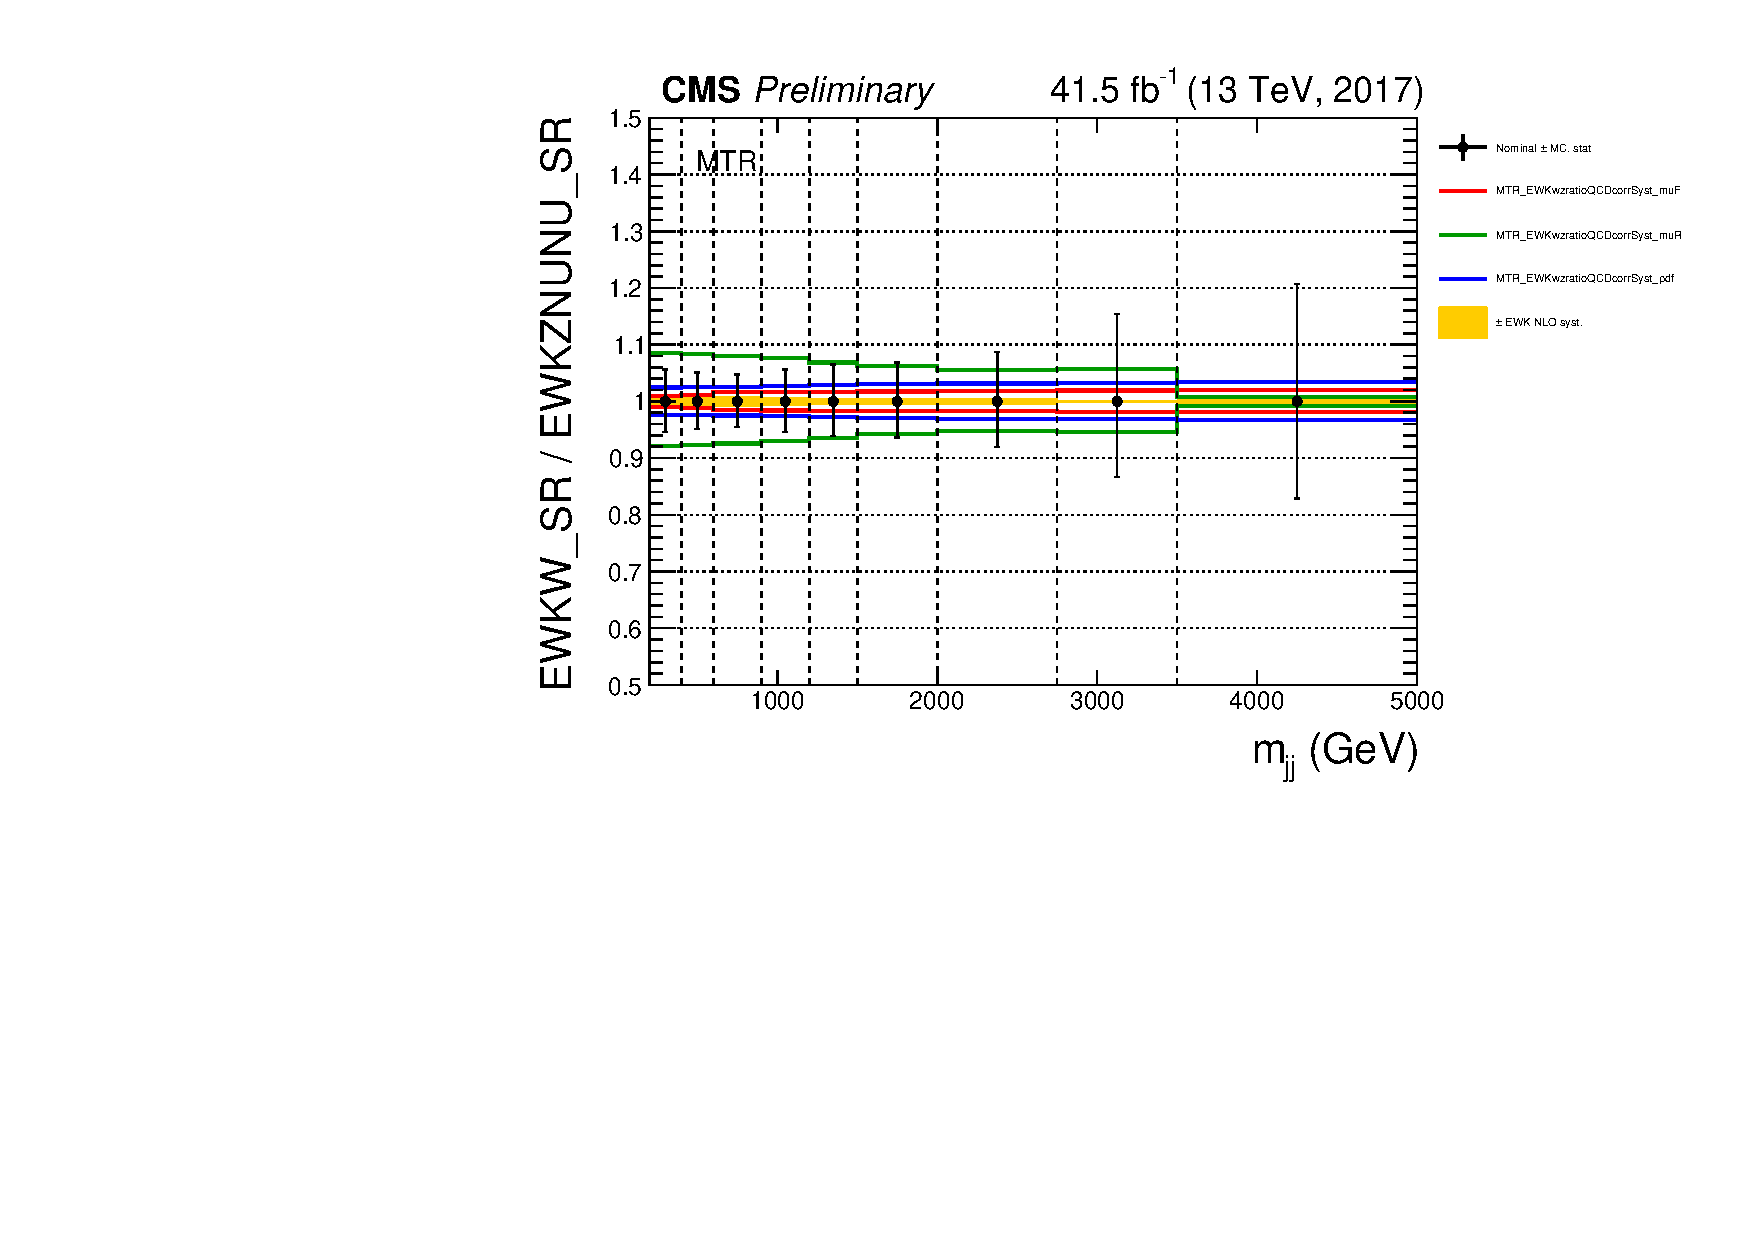
\includegraphics[width= 0.8\textwidth]{FIt_structure/VBF_MTR_2017_EWKW_SR_EWKZNUNU_SR.pdf}}\\
    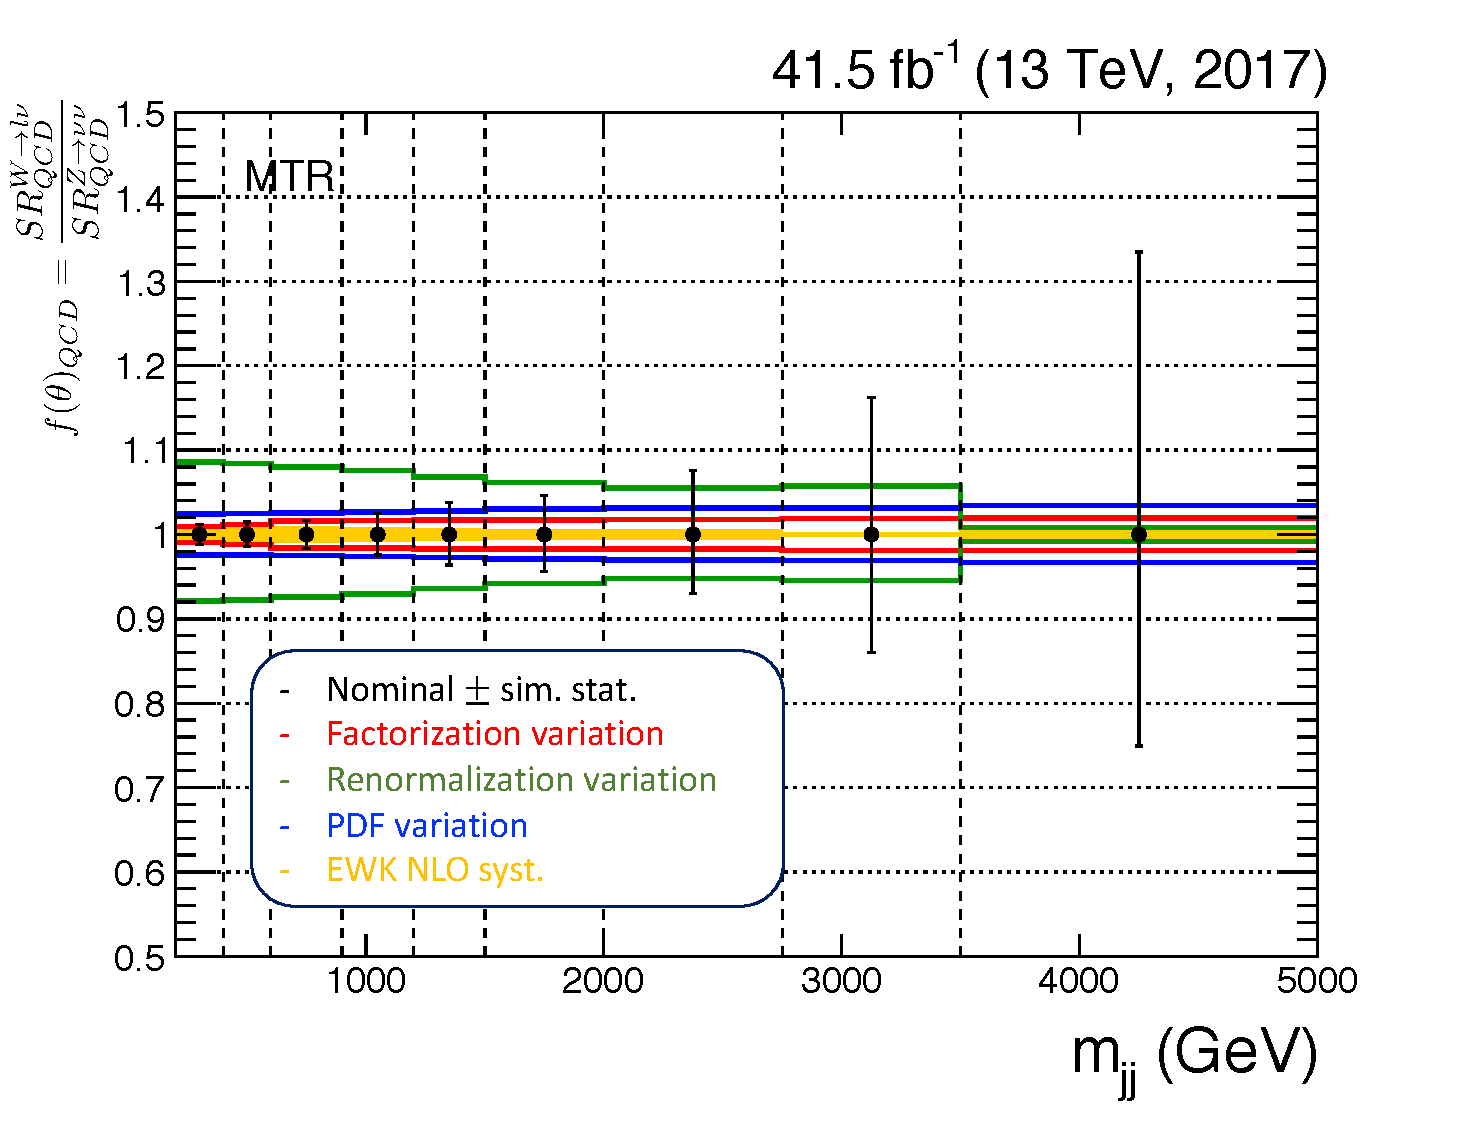
\includegraphics[width= 0.8\textwidth]{FIt_structure/theory_uncert_MTR_2017.pdf}
    
  \caption{Theoretical uncertainties on $f(\boldsymbol{\theta})$ ratios for the MTR category and 2017 data, presented as a function of $m_{jj}$ for the QCD production modes.}
  \label{fig:theory_MTR_2017}
\end{figure}




%As these corrections are being applied as a two dimensional weight map in generator level boson $p_T$ and $m_{jj}$ (as discussed in Chapter~\ref{ch:objects}), the final uncertainties are derived through the differences between the NLO cross sections (expressed in boson $p_T$ and $m_{jj}$) corresponding to the variated and nominal scenario. Finally, the uncertainty originating from the PDF modelling is estimated through a procedure recommended by the PDF4LHC working group~[R] and combined with other sources through a squared sum. 
 
\subsection{Experimental uncertainties}
\hspace{10pt} The experimental uncertainties trace their origin to the effects of the performance of the detector and the object reconstruction. Sources comprising this group include pileup re-weighting, trigger performance, jet energy corrections (both the scale and resolution) and object reconstruction and isolation criteria (expressed through the usage of selection/veto weights as explained in Chapter~\ref{ch:objects}).


\hspace{10pt} The uncertainties on the V+jets transfer factors are summarised in Table~\ref{tab:systematics}. Following the odering presented in the aforementioned table, this discussion can start with the trigger efficiencies. The uncertainty of the electron trigger efficiencies has been measured to have an 1\% effect on the relevant electron transfer factors. The VBF and $E_{T,miss}$ triggers, being used to form muon CRs and SR, add 2~\% and 10\% uncertainties on the SR and muon transfer factors, respectively.

\hspace{10pt} The next group of uncertainties is associated with the lepton reconstruction, identification and isolation efficiencies taking into account uncertainties of the ($p_T,\eta$) scale factors introduced with Equation~\ref{eq:sel_weight}, resulting in per-lepton uncertainties for the muons (0.5~\% for the identification and 0.1~\% for the isolation efficiency) and electrons (0.5~\% for the reconstruction and 3~\% for the combined identification/isolation efficiency)\footnote{Being relevant for the corresponding SR to lepton CR transfer factors.}. Equivalent approach is taken for the veto weights introduced for the simulated background samples when defining the SR (as introduced with Equation~\ref{eq:veto_weight}). These include a set of uncertainties arising from tau (1\%), muon (0.5\%) and electron (3\% from identification/isolation and up to 1.5~\% from the reconstruction) vetos.


\hspace{10pt} The last group of uncertainties relevant to the V+jets transfer factors is related to the uncertainty of the simulation modelling of $E_{T,miss}$~\cite{paper:met_performance}. The dominating effects arise form the jet energy scale and resolution. Their effect is estimated by taking into account each of these corrections, which translates into variations of momenta within the jet collection and are, as a consequence, propagated to the $E_{T,miss}$ computation. Tests from the perspective of the analysis\footnote{Important as these changes can lead to a different set of jets being chosen as the desirable pair.} led to the conclusion that these effects mostly cancel in the transfer factors leaving a residuum summarised in Table~\ref{tab:systematics} where these uncertainties are separated by its source and the affecting transfer factor.


\hspace{10pt} Lastly, minor contributions form other SM background such as the top, QCD multijet and diboson processes enter the likelihood function as shown in Equations~\ref{eq:likelihood_sr}-\ref{eq:likelihood_singlelep}. Their associated uncertainties are summarised in Table~\ref{tab:systematics_minor} denoting the affected SM process and the region in which the uncertainty becomes relevant.


\begin{table}[htbp]

\small
    \begin{center}
       \begin{tabular}{llc}
       \hline
       \hline
       Source                    & Process                                    & Uncertainty  \\
       \hline
       \hline
       Electron  trigger         & $W_{SR}/W_{e\nu}$, $Z_{\nu\nu}/Z_{ee}$       & 1\% \\
       \MET   triggers (MTR)            & $W_{SR}/W_{CR}$, $Z_{\nu\nu}/Z_{CR}$, $Z/W$, signal & 2\% \\
       VBF  triggers (VTR)            &  $W_{SR}/W_{CR}$, $Z_{\nu\nu}/Z_{CR}$, $Z/W$, signal   & 10\% \\
%       Photon  trigger           & $Z_{\nu\nu}/\gamma$                           & 1\% \\
       \hline
       Muon-ID   efficiency      & $W_{SR}/W_{\mu\nu}$, $Z_{\nu\nu}/Z_{\mu\mu}$ & 0.5\% (per muon) \\
       Muon-Iso   efficiency     & $W_{SR}/W_{\mu\nu}$, $Z_{\nu\nu}/Z_{\mu\mu}$ & 0.1\% (per muon) \\
       Electron-reco efficiency  & $W_{SR}/W_{e\nu}$, $Z_{\nu\nu}/Z_{ee}$       & 0.5\% (per electron) \\
       Electron-IDiso efficiency & $W_{SR}/W_{e\nu}$, $Z_{\nu\nu}/Z_{ee}$       & 3\% (per electron) \\
 %      Photon-IDiso efficiency   & $Z_{\nu\nu}/\gamma$       & 5\% \\
      \hline
      Electron veto from reco &  $W_{SR}/W{CR}$, $Z/W$  & 1\% (QCD), 1.5\% (EW)\\
      Electron veto from idiso &  $W_{SR}/W{CR}$, $Z/W$  & 3\% \\
      Muon veto &  $W_{SR}/W{CR}$, $Z/W$  & 0.5\% \\
      Tau veto &  $W_{SR}/W{CR}$, $Z/W$  & 1\% \\
      \hline
       \multirow{3}{*}{Jet energy scale}         & $Z/W$         & 1--2\%\\
                                & $W_{CR}/W_{SR}$               & 1.0--1.5\% \\
                               	& $Z_{CR}/Z_{\nu\nu}$   		& 1\% \\\hline
 %                              	& $Z_{\nu\nu}/\gamma$	    	& 3\% \\\hline
       \multirow{3}{*}{Jet energy resolution}  	& $Z/W$         & 1.0--2.5\% \\ 
                                & $W_{CR}/W_{SR}$               & 1.0--1.5\% \\
                                & $Z_{CR}/Z_{SR}$				& 1\% \\
 %                               & $Z_{\nu\nu}/\gamma$	    	& 1--4\% \\
       \hline
       %pileup & all ratios & 1\% \\
      \end{tabular}
    \end{center}
        \caption{Summary of experimental uncertainties on the transfer factors for main V+jets backgrounds. Where specified in the form of a range of values, the values vary with era of data taking (or transfer factors).}
    \label{tab:systematics}
\end{table}


\begin{table}[htbp]

\small
    \begin{center}
       \begin{tabular}{llc}
       \hline
       \hline
       Source                    & Process                                    & Uncertainty  \\
       \hline
       \hline
       Luminosity                & All & $\approx$~2.5~\%\\
       Pile-up                & All & up to 3~\%\\
       Electron  trigger         & All in Z(ee) and W(e$\nu$)     & 1~\% \\
       \MET~triggers             & All in Z($\mu\mu$),W($\mu\nu$) and SR (MTR) & 2~\% \\
       VBF  triggers             & All in Z($\mu\mu$),W($\mu\nu$) and SR (VTR)  & 10~\% \\
       Level-1 pre-fire  & All (2017 only) & 3~\%\\
%       Photon  trigger           & $Z_{\nu\nu}/\gamma$                           & 1\% \\
       \hline
       Muon-ID   efficiency      &  All in Z($\mu\mu$),W($\mu\nu$) & up to 2~\% \\
       Muon-Iso   efficiency     &  All in Z($\mu\mu$),W($\mu\nu$)  & up to 0.5~\%\\
       Electron-reco efficiency  &  All in Z(ee) and W(e$\nu$)       & up to 1~\% \\
       Electron-IDiso efficiency &  All in Z(ee) and W(e$\nu$)       & up to 3~\% \\
 %      Photon-IDiso efficiency   & $Z_{\nu\nu}/\gamma$       & 5\% \\
      \hline
      Electron veto from reco & All in SR  & up to 1.5~\%\\
      Electron veto from IDiso & All in SR  & up to 5~\%  \\
      Muon veto &  All in SR  & up to 0.5~\% \\
      Tau veto &  All in SR and CR & up to 1~\% \\
      \hline
       Jet energy scale         & All          & 10\%\\
 %                              	& $Z_{\nu\nu}/\gamma$	    	& 3\% \\\hline
       Jet energy resolution  	& All       & 0.5--5\%\\ 
       QCD estimation 	& QCD MTR (VTR)     & 40 (10)\%\\ 
 %                               & $Z_{\nu\nu}/\gamma$	    	& 1--4\% \\
       \hline
       %pileup & all ratios & 1\% \\
      \end{tabular}
    \end{center}
    \caption{Summary of experimental uncertainties affecting smaller backgrounds.}
    \label{tab:systematics_minor}
\end{table}

\section{QCD estimation}
\hspace{10pt} The commonly used method when estimating the contribution of QCD multijet processes in the SR is the Method A, introduced in~Section~\ref{sec:qcd_a}. Its reliance on simulated multijet events and their lack of statistical precision led to the method's limited usability, especially when it comes to the VTR category.

\hspace{10pt} This is a consequence of the core idea of establishing the connection between the QCD CR and SR trhough the use of the $r(m_{jj})$ factor, which is estimated using simulated events. This is illustrated in Figure~\ref{fig:qCD_A_ratio}, which shows an attempt to salvage this method by relaxing the $\Delta \phi_{jj}$ requirement in steps of 0.2 until 2.5 from the perspective of the MTR category.

\begin{figure}[htbp]
  \centering
    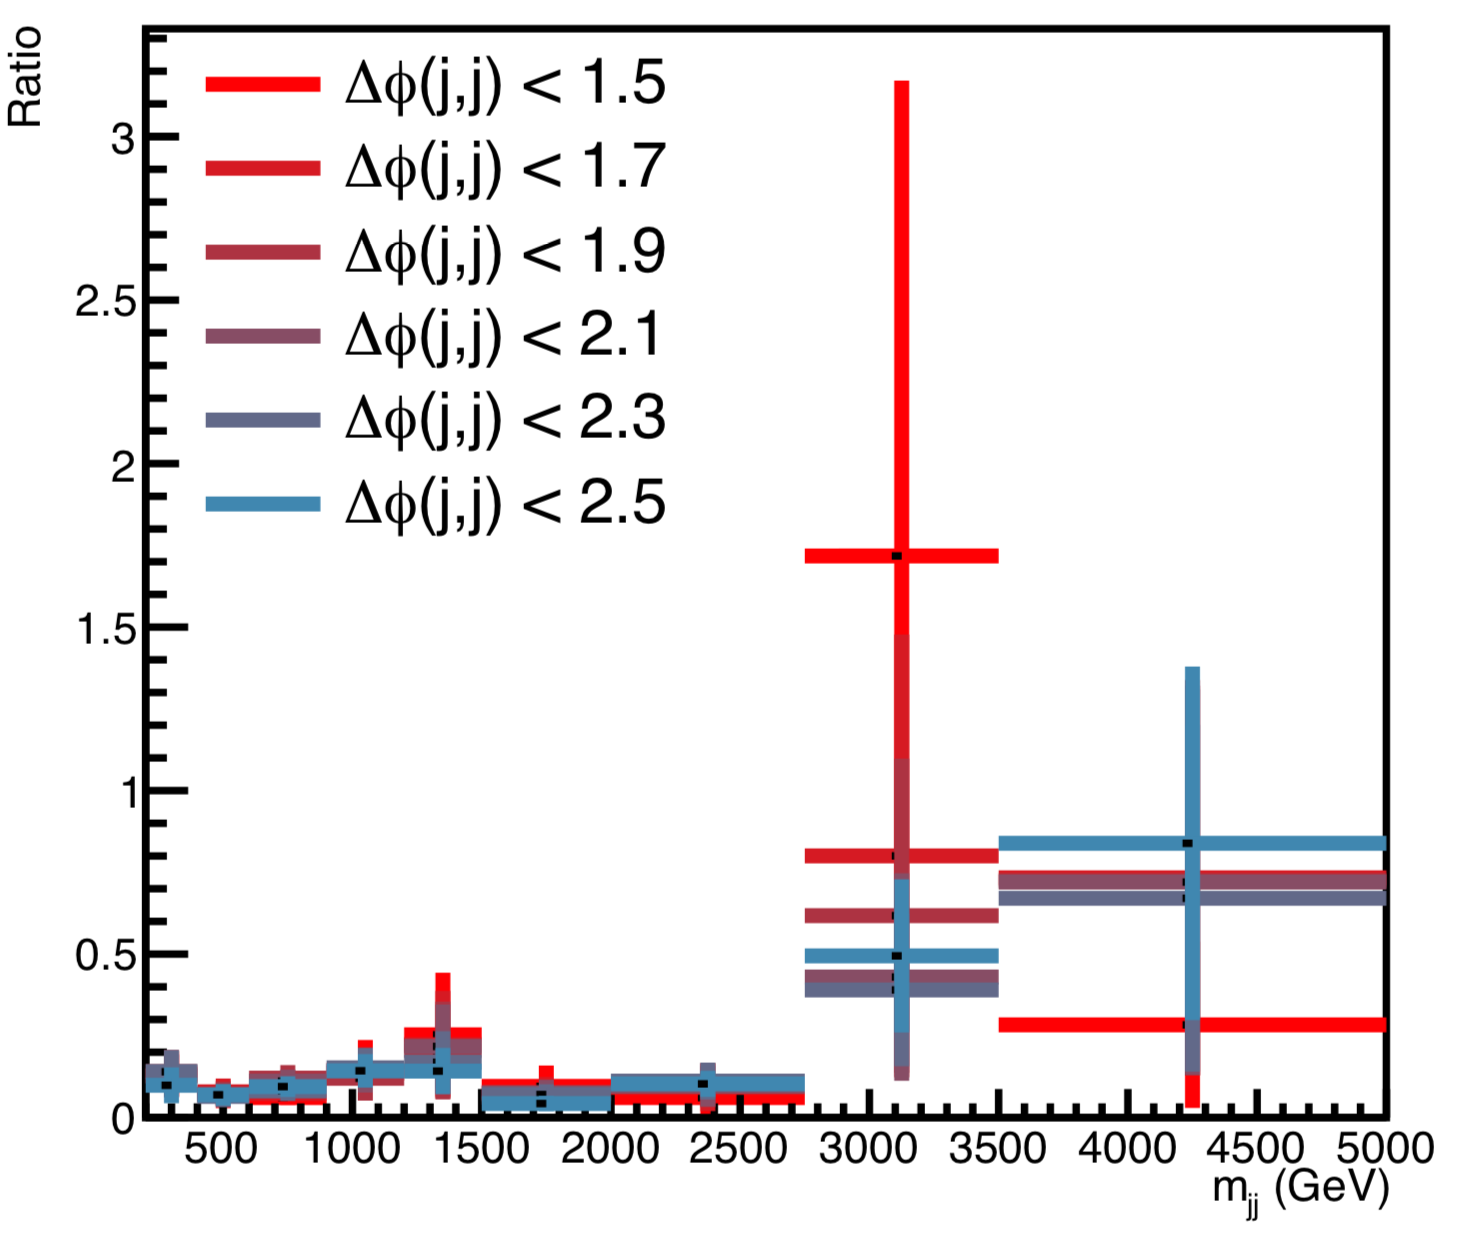
\includegraphics[width= 0.7\textwidth]{FIt_structure/qcd_a_relaxed.png}
  \caption{Various distributions of the ratio $r(m_{jj})$ shown for a range of $\Delta\phi_{jj}$ thresholds.}
  \label{fig:qCD_A_ratio}
\end{figure}


\hspace{10pt} The alternative method, method B, was introduced to mitigate the issues which arise due to the dependency on simulation samples. It instead, as defined in Section~\ref{sec:qcd_b}, relies on a mostly data driven approach when estimating the final multijet contribution. This is achieved by using a data driven method of estimating the normalisation of the multijet processes in the SR by fitting the $min\Delta\phi(j, E_{miss})$ variable for data and minor backgrounds. This in return gives a function describing the behaviour of the multijet processes in QCD CR: $F_{QCD}(x) = F(x) - F_{B}(x)$\footnote{Using the notation introduced in Section~\ref{sec:qcd_b}, where x~$= min\Delta\phi(j, E_{miss})$.}.

\hspace{10pt} This function can be extrapolated to the SR and integrated within the SR defined region of $min\Delta\phi(j, E_{miss})$, giving an estimate on the normalisation. The final step is to extract the $m_{jj}$ shape of multijet processes from the QCD CR and scale it to the correct SR normalisation. This is performed under the assumption that the QCD CR defining variable ($min\Delta\phi(j, E_{miss})$) and $m_{jj}$ are not strongly correlated\footnote{This assumption is further supported by the small variation of the value of $r(m_{jj})$ for bins with higher statistical precision (as indicated with Figure~\ref{fig:qCD_A_ratio}).}.

%\hspace{10pt} Figure~\ref{fig:qcd_b_midphi_2017} shows the first step - the fitting procedure of the min$\Delta \phi (j, E_{T,miss})$ variable used to extract the total yield of multijet processes in the SR (presented for the MTR category for both 2017 and 2018 data). The fit range is defined to reach min$\Delta \phi (j, E_{T,miss})<$~1 (1.5) for MTR (VTR) categories. Similarly, the control region used to compare the quality of the fit is defined from the end of the fit range until 1.2 (1.8) for MTR (VTR). This was made possible as a result of the unblinding strategy being put in place in order to mitigate the effects of jet horns and HEM problems (as described in Chapter~\ref{sec:data_quality}), with the extended range being supported with the assumption that no significant signal contribution is expected bellow those values. 

%\hspace{10pt} These distributions present data (black points), sum of minor backgrounds (blue points), multijet simulated events (red points - only for comparison, not being used anywhere) and the fit functions for the data ($F(x)$ - dashed black line), minor backgrounds ($F_{B}(x)$ - dashed blue line) and the multijet estimation ($F_{QCD}$ - dashed red line). Additionally, a sum of the contributions from minor backgrounds combined with $F_{QCD}$ is presented (solid magenta line).

%\hspace{10pt} The bottom panel focuses on the ratios between the fit functions and their corresponding processes. This includes a comparison of $F(x)$ versus data (expressed with black color), which shows a good agreement above the fit range. Additional comparisons are made between the $F_{B}$ and the sum of minor background processes (blue) as well as the $F_{QCD}$ versus multijet simulated events (red - but, similar to above, only for illustration purposes).

%\begin{figure}[htbp]
%  \centering
%    \subfigure[MTR 2017]{\includegraphics[width= 0.65\textwidth]{Results/{out_MTR_2017.root_qcdDD_normfit}.pdf}}\\
%    \subfigure[MTR 2018]{\includegraphics[width= 0.65\textwidth]{Results/{out_MTR_2018.root_qcdDD_normfit}.pdf}}
%  \caption{Extraction of the overal normalisation of the SR contribution originating from QCD multijet processes obtained through the use of Method B for the MTR category for (a) 2017 and (b) %2018 data.}
%  \label{fig:qcd_b_midphi_2017}
%\end{figure}
 
\hspace{10pt} The final prediction from this method, obtained by scaling the estimation of the multijet $m_{jj}$ shape from the QCD CR to the SR normalisation, is shown in Figure~\ref{fig:qcd_b_mjj_2017} for the MTR category for both 2017 and 2018 data. A comparison with the results originating from Method A is also presented (magenta line) as well as the prediction from QCD multijet simulated events (red). As the method relies on the extended CR range enabled though the unblinding of 20~\% of data, the final shape needed to be further scaled up by a factor of 5 until the analysis was fully unblinded. Lastly, the uncertainty of this prediction arises from the normalization fit error and stands at 40~\% (10~\%) for MTR (VTR) category. This is propagated as a flat uncertainty on this prediciton when it is passed on as an input for the signal extraction fit. %Figure~\ref{app:qcd_comp}

\begin{figure}[htbp]
  \centering
    \subfigure[MTR 2017]{\includegraphics[width= 0.7\textwidth]{Results/{out_MTR_2017.root_qcdDD}.pdf}}\\
    \subfigure[MTR 2018]{\includegraphics[width= 0.7\textwidth]{Results/{out_MTR_2018.root_qcdDD}.pdf}}
  \caption{Final estimation of the SR contribution originating from QCD multijet processes obtained through the use of Method B for the MTR category for both (a) 2017 and (b) 2018 data.}
  \label{fig:qcd_b_mjj_2017}
\end{figure}




\newpage

\section{Results}

\hspace{10pt} The signal extraction procedure introduced in previous sections is applied to all regions simultaneously, allowing the fit to access all available data taking periods and categories. This section summarises final results, expressed in terms of the 95~\% CL upper limit on Br(H$\rightarrow$~inv)\footnote{As no significant deviations from the SM have been observed.} for all analysis categories. In order to formulate a preliminary look at the combined Run 2 (or the "legacy") result, a combination is performed with the studies targeting the 2016 data without re-analysing the data (explained in great detail in Refs.~\cite{paper:HIG_17_023,Riccardo}).

\hspace{10pt} Treatment of the most important nuisance parameters, such as the ones related to lepton efficiencies, have been left uncorrelated between the three years with the uncertainties assigned to the jet energy scale and resolution also following the uncorrelated path reflecting the different operational conditions of the CMS experiment. A correlation between theory uncertainty has been established between 2017 and 2018 (although they differ between MTR and VTR categories). Lastly, the addition of the photon region has been performed for the MTR category for the 2017 and 2018 eras of data taking.


%The fit procedure taken for this approach is the "S+B" fit, which allows for the SR information to be included in the input (as indicated in the definition of the likelihood functions)

\hspace{10pt} Starting with the main analysis category, Figures~\ref{fig:MTR_2017_CR} and \ref{fig:MTR_2018_CR} show post-fit distributions for the MTR CRs. These distributions show the data versus simulated background composition for the lepton/photon regions (with the background contributions being presented with their post-fit predictions). The ratio panel is used to show data to simulation ratio for both the pre-fit (red) and post-fit (black) scenarios. The corresponding distributions for the VTR category are shown in Figures~\ref{fig:VTR_2017_CR} and \ref{fig:VTR_2018_CR}. Concluding this set, post-fit distributions of the SR for all categories and data taking periods are shown in Figure~\ref{fig:SR}\footnote{The post-fit distributions from the fit procedure which uses the "CR-only" approach (by using the data from CRs only) are shown in Figures~\ref{app:MTR_2017_CR}-\ref{app:SR}.}. Tables~\ref{app:MTR_2017_yield}-\ref{app:MTR_2018_yield} (\ref{app:VTR_2017_yield}-\ref{app:VTR_2018_yield}) present the final yields in the SR for the MTR (VTR) category. The summary of the main nuisance parameter impacts for the combined fit (depicting 2017 and 2018 data) are shown in Figures~\ref{app:impacts_MTR_2017}-\ref{app:impacts_VTR_2018}. The leading nuisance parameters (for both MTR and VTR categories), ordered by their influence over the Br(H$\rightarrow$inv), are the ones related to statistical precision of the simulation samples, theory corrections and trigger scale factors. Looking into the per-category summaries shown in the aforementioned figures, it can be seen that the parameter that is most significantly pulled by the fit for both the MTR 2017 and 2018 categories ("$\text{qcd\_photon\_ewk\_vbf\_*}$")\footnote{With the pull being defined as the difference between the post and the pre-fit value of a nuisance parameter divided by its uncertainty.} is related to the theory uncertainties associated to the photon CR. The necessity for the pull came from the fit procedure adjusting the prediction to the reality seen in data, but it is still low enough ($\sim$1~$\sigma$) to raise any concerns regarding the photon region. For the MTR 2018 category, there is one more parameter that is largely pulled by the fit - "$\text{vbf\_2018\_stat\_error\_qcd\_photonCR\_*}$", related to the statistical precision of the photon region, but its importance to the Br(H$\rightarrow$inv) is small enough that its large pull isn't an indication of a problem. For the VTR category, there aren't any highly pulled nuisance parameters. One difference for these categories (as compared to the MTR) is that the nuisance parameters related to the trigger algorithms have a much larger role from the Br(H$\rightarrow$inv) point of view.


\begin{figure}[htbp]
  \centering
   \subfigure[Dimuon CR]{ 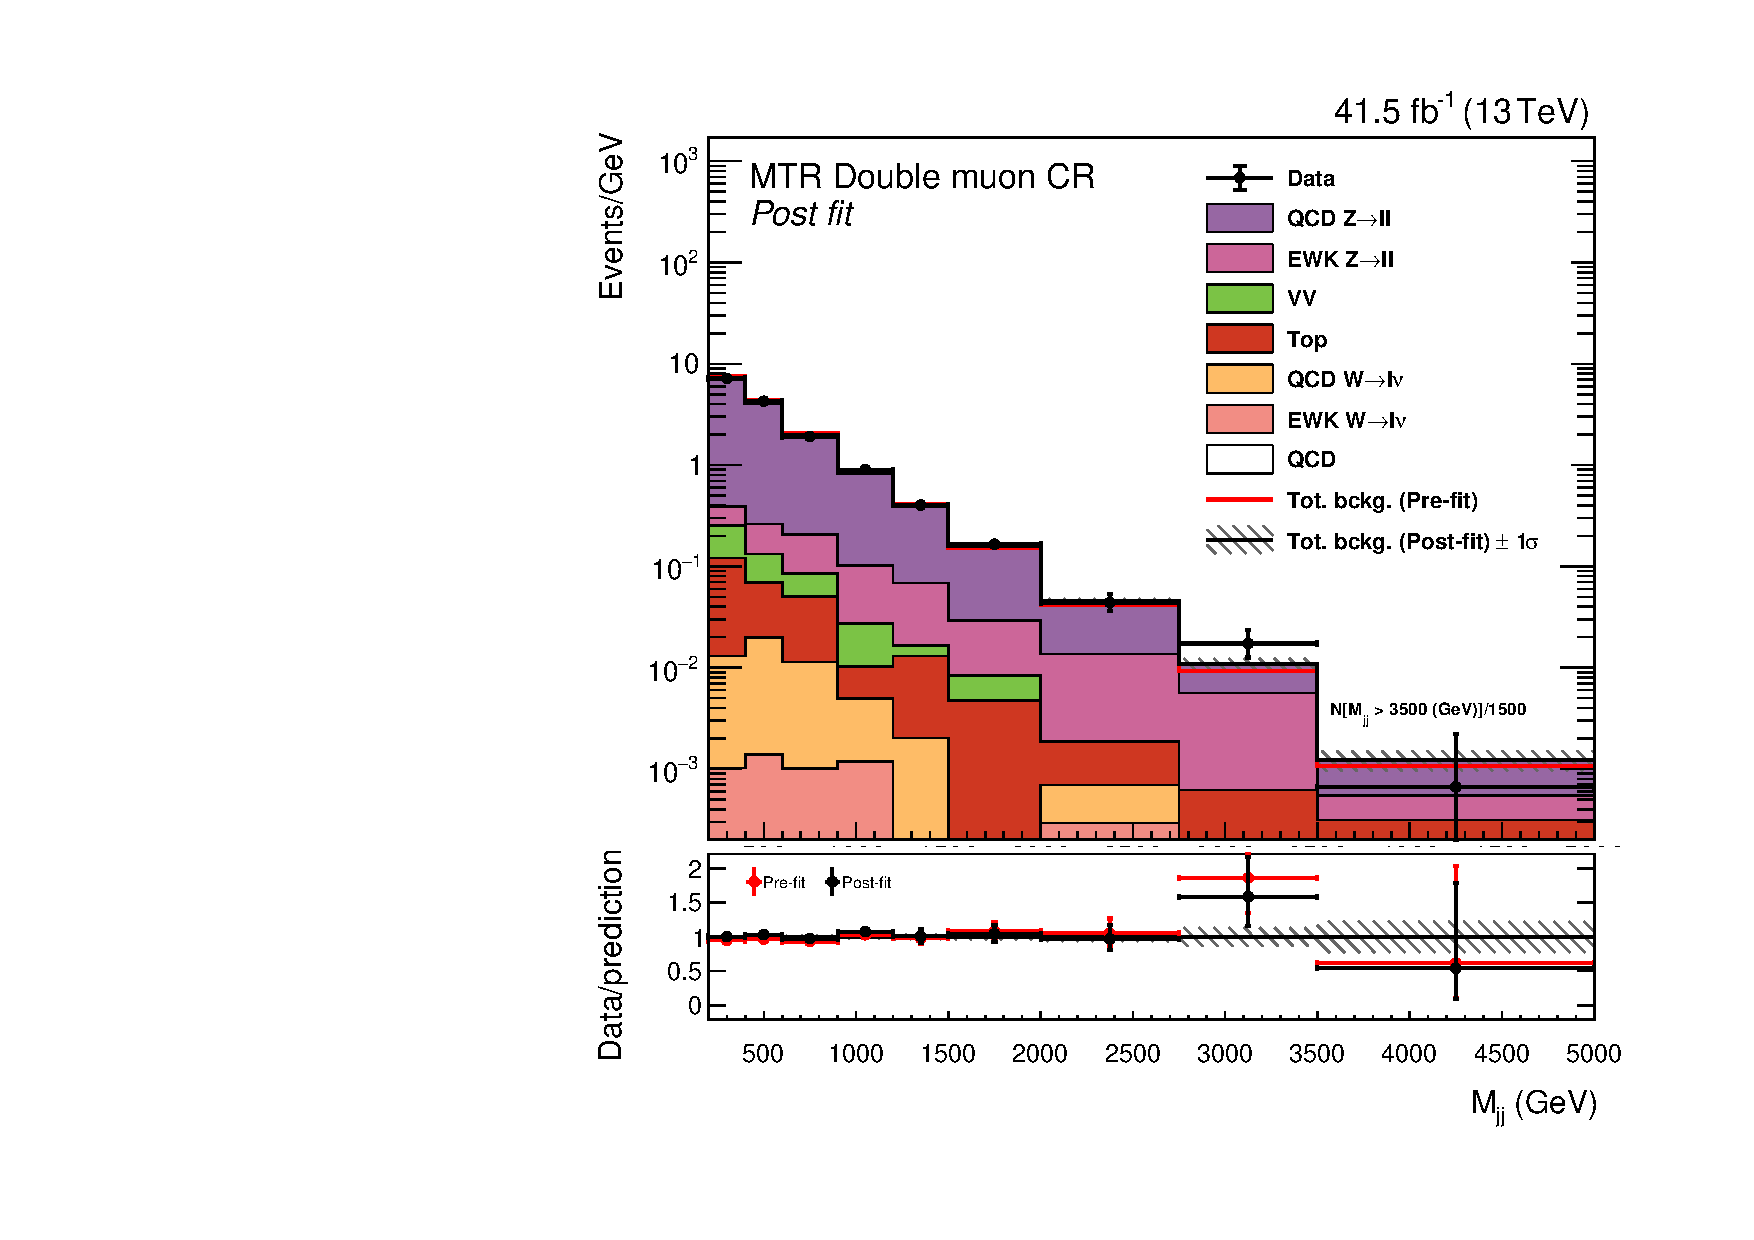
\includegraphics[width= 0.47\textwidth]{Results/SplusBFit/MTR_2017_ZMUMU.pdf}}
     \subfigure[Dielectron CR]{ 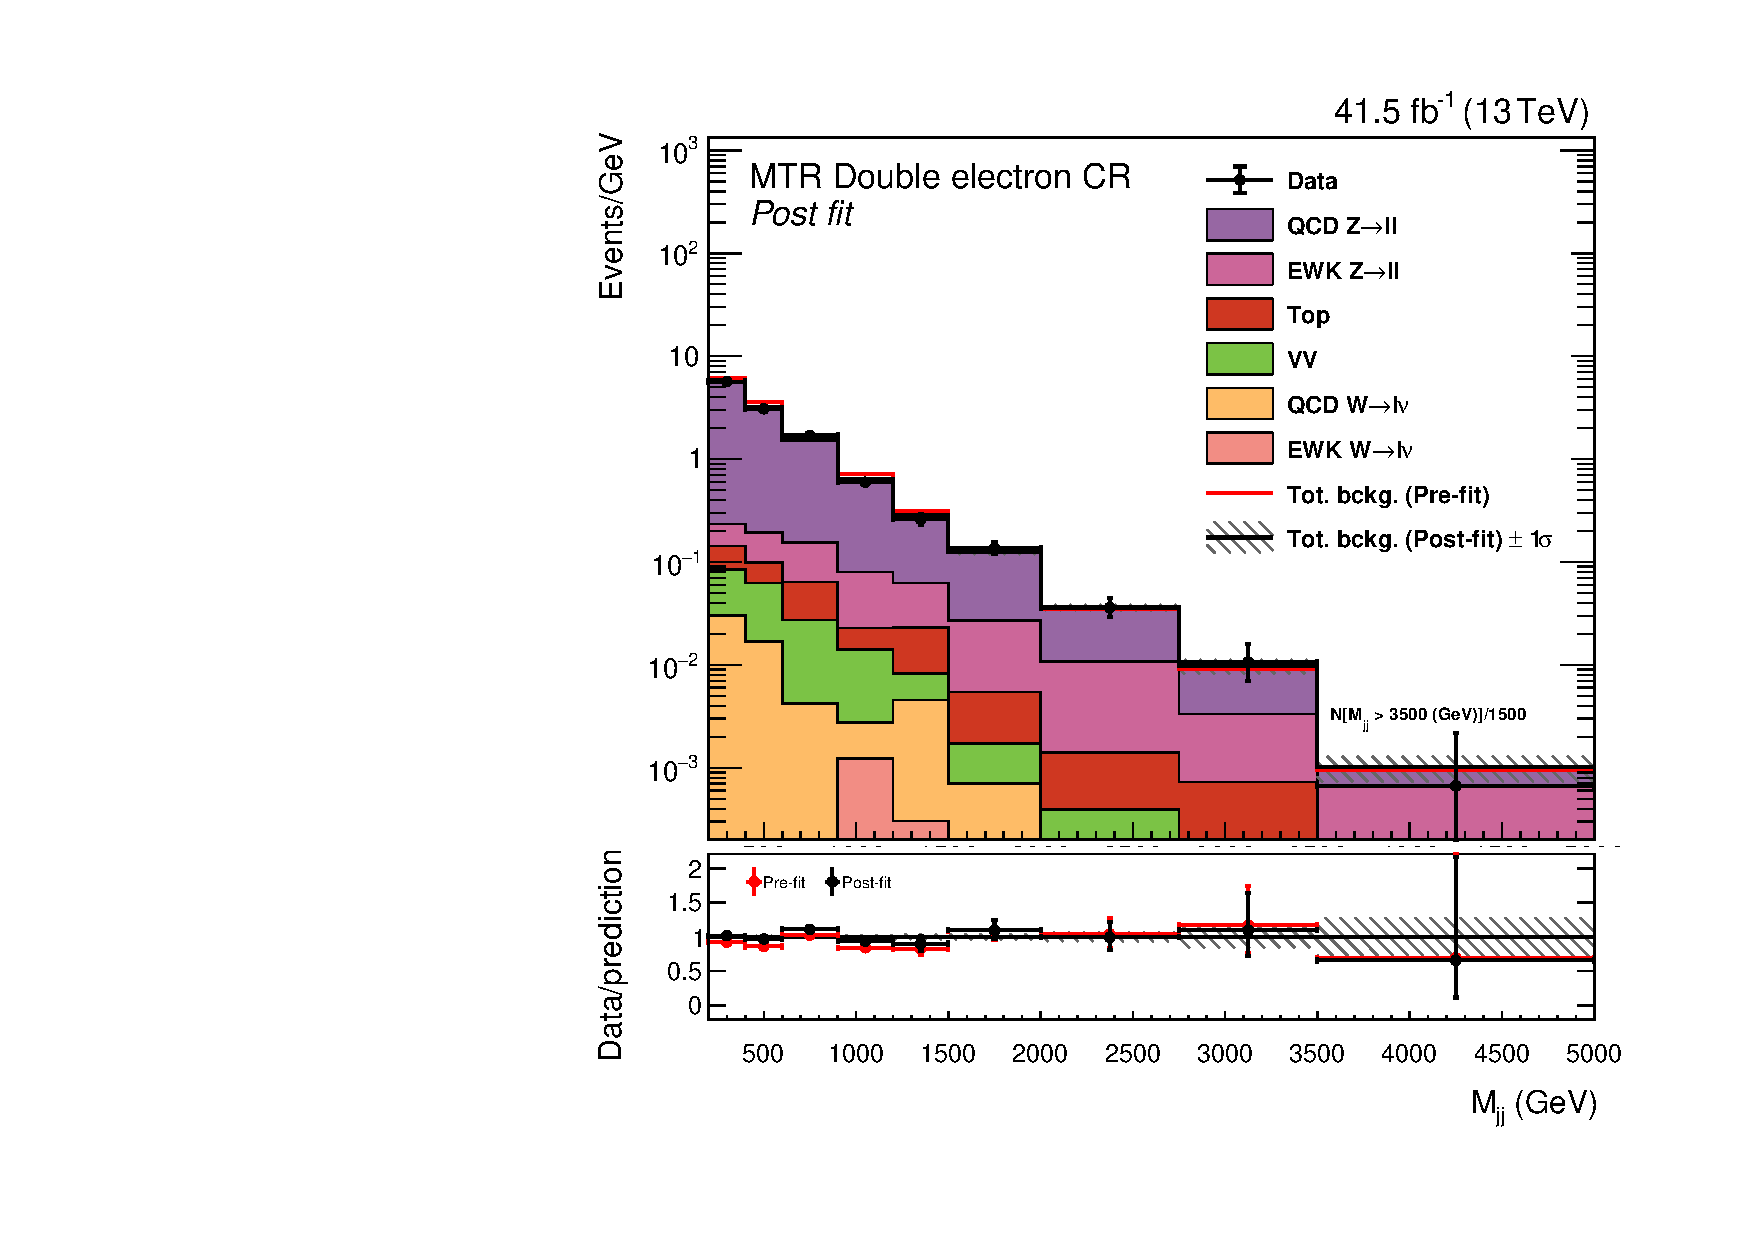
\includegraphics[width= 0.47\textwidth]{Results/SplusBFit/MTR_2017_ZEE.pdf}}\\
     \subfigure[Single muon CR]{ 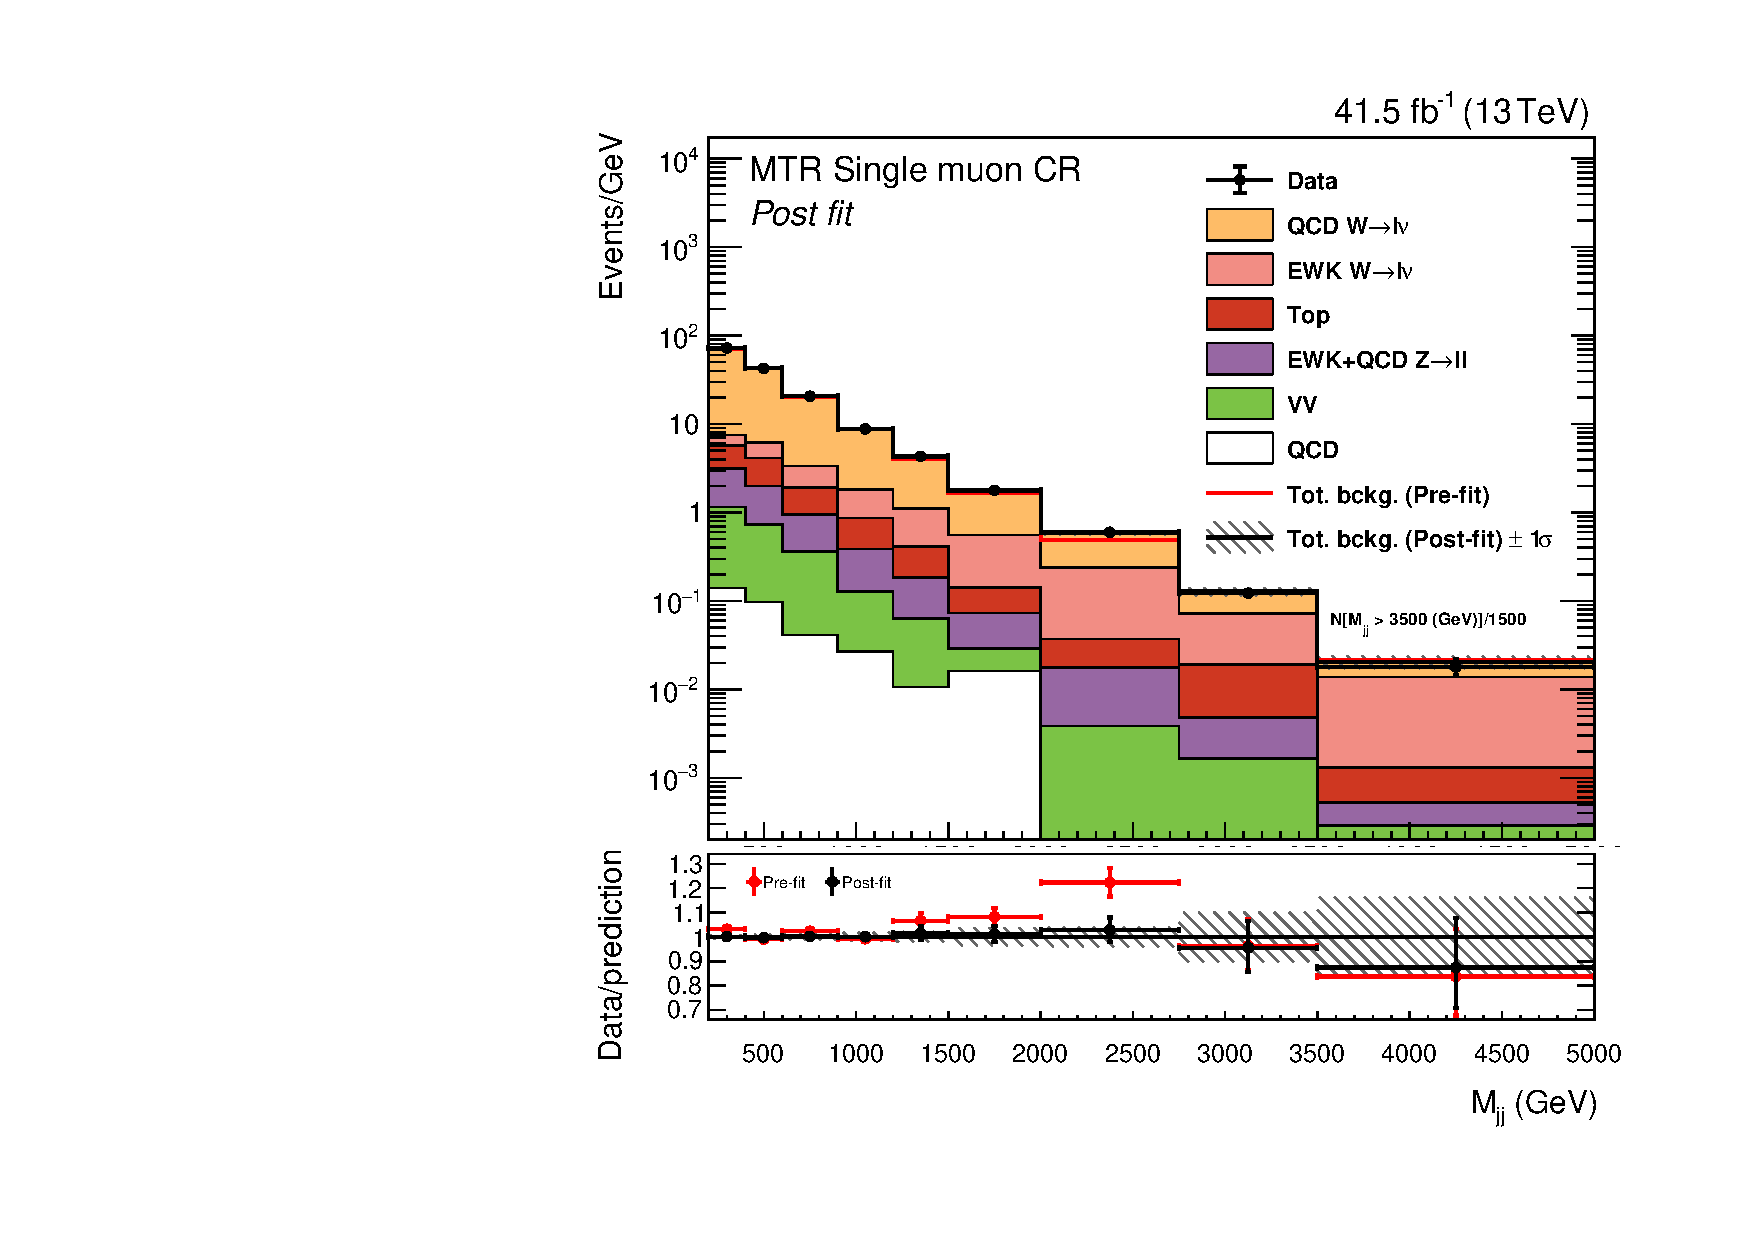
\includegraphics[width= 0.47\textwidth]{Results/SplusBFit/MTR_2017_WMUNU.pdf}}
    \subfigure[Single electron CR]{
    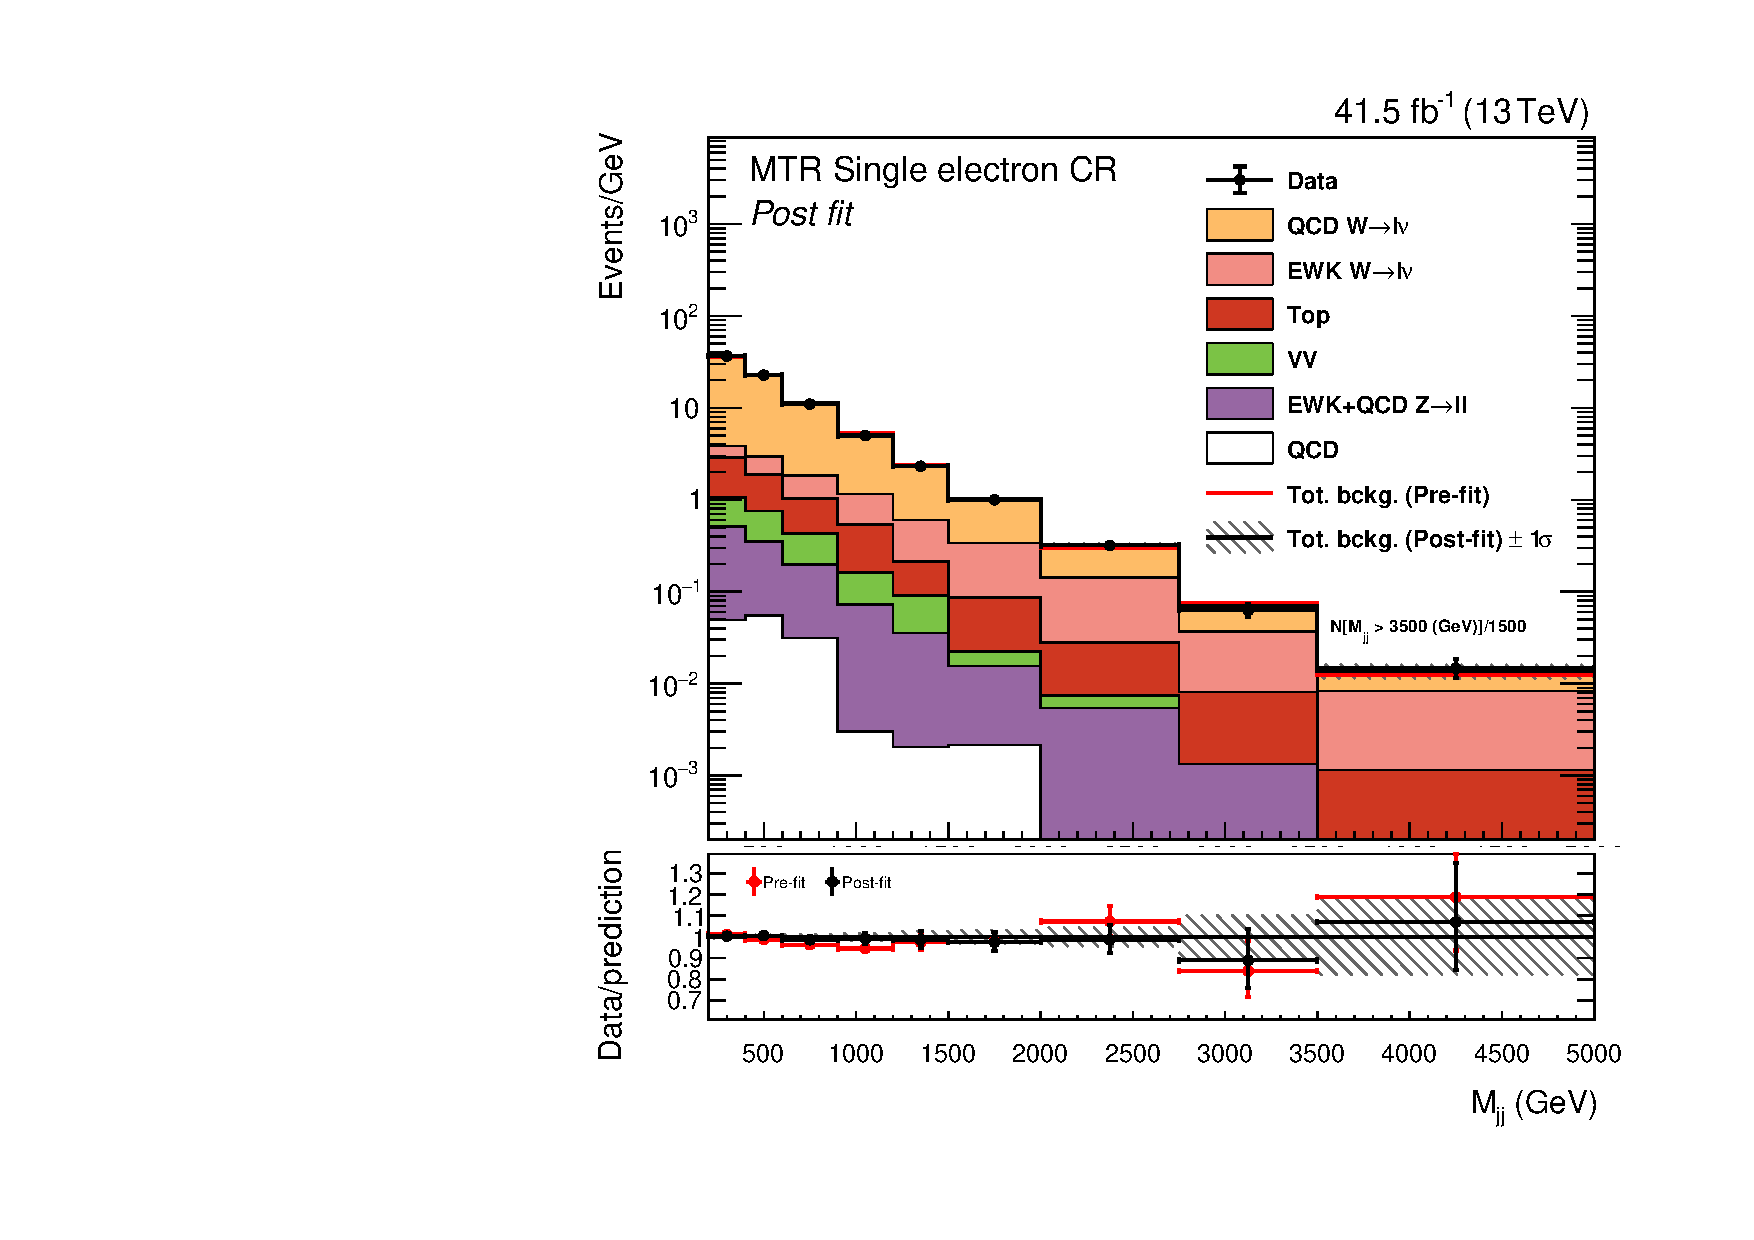
\includegraphics[width= 0.47\textwidth]{Results/SplusBFit/MTR_2017_WENU.pdf}}\\
      \subfigure[Photon CR]{
    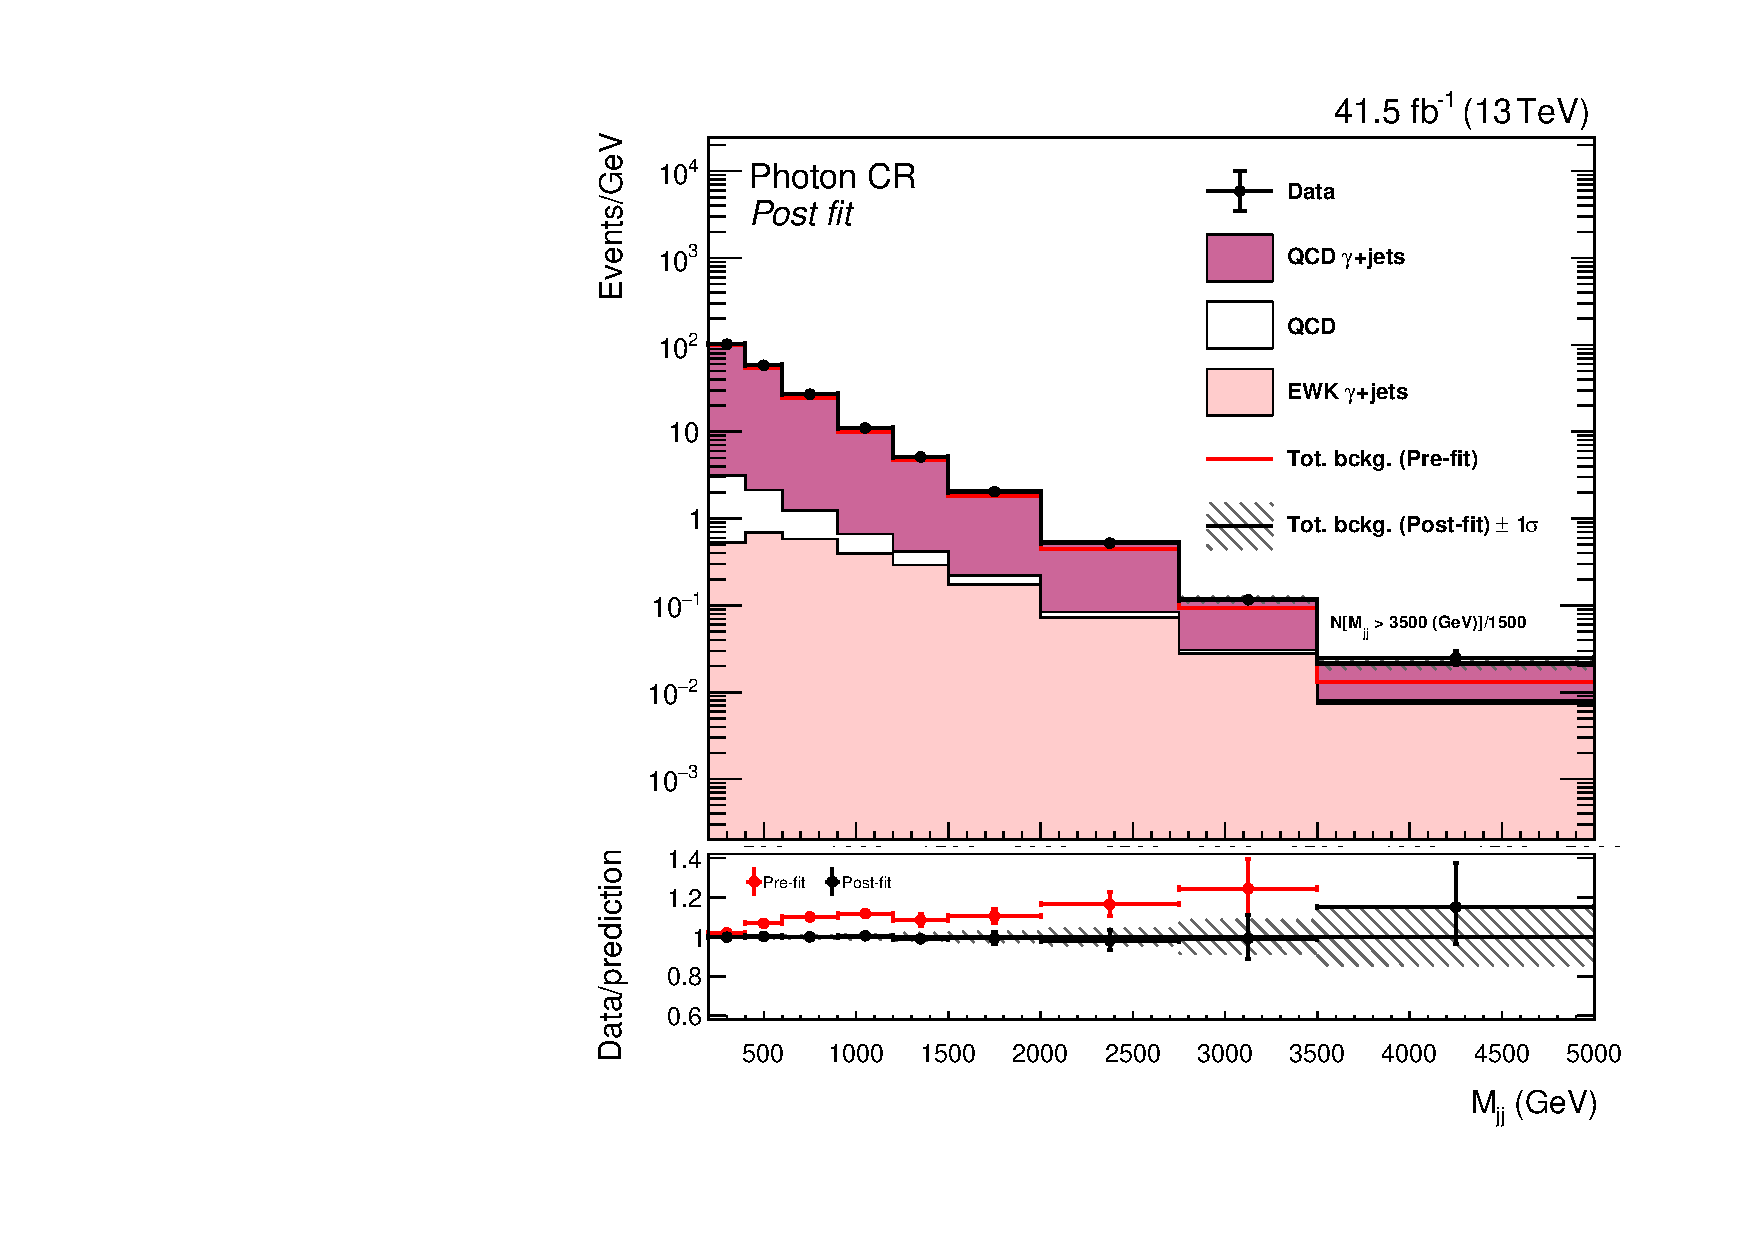
\includegraphics[width= 0.47\textwidth]{Results/SplusBFit/photon_cr_2017.pdf}}
  \caption{Post-fit distributions for 2017 data, showing the: (a) dimuon, (b) dielectron, (c) single muon, (d) single electron and (e) photon CR region.}
  \label{fig:MTR_2017_CR}
\end{figure}


\begin{figure}[htbp]
  \centering
   \subfigure[Dimuon CR]{ 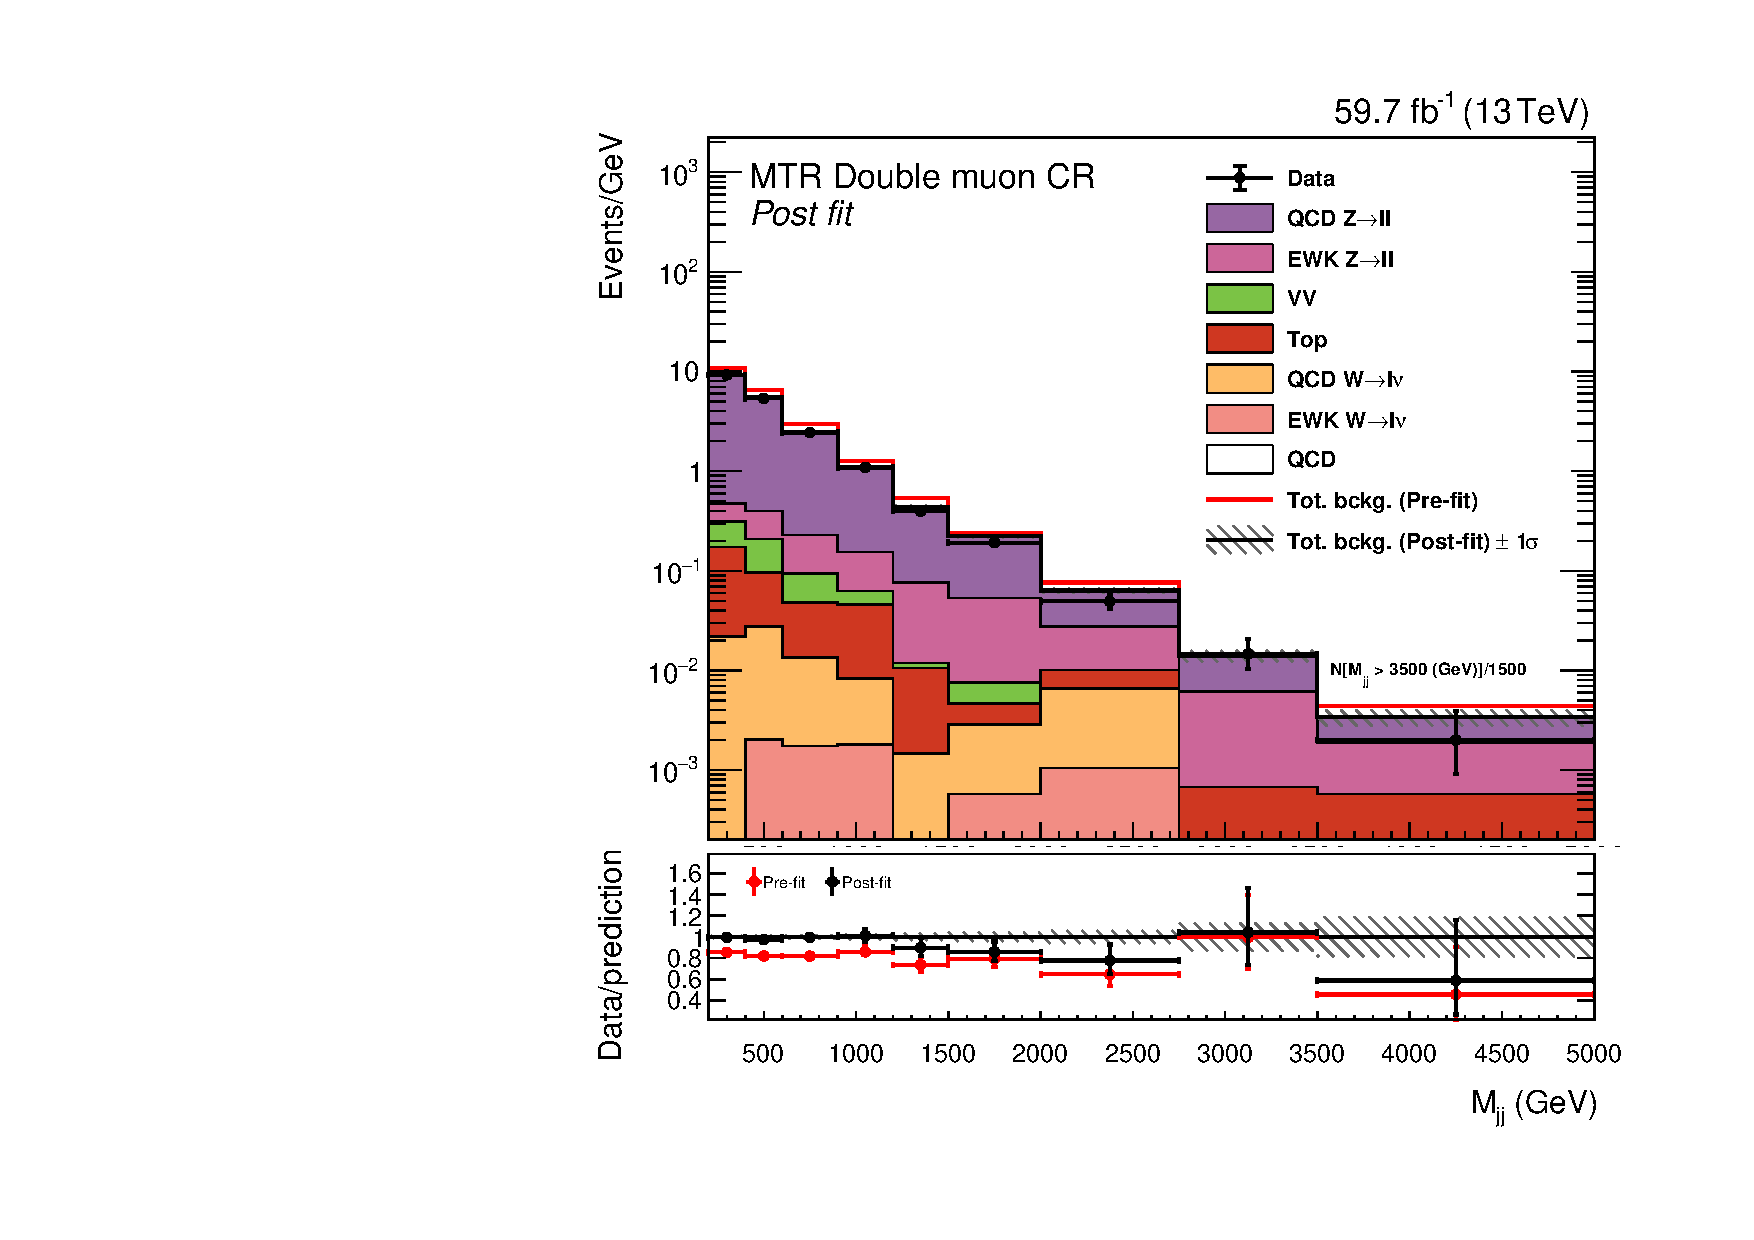
\includegraphics[width= 0.47\textwidth]{Results/SplusBFit/MTR_2018_ZMUMU.pdf}}
     \subfigure[Dielectron CR]{ 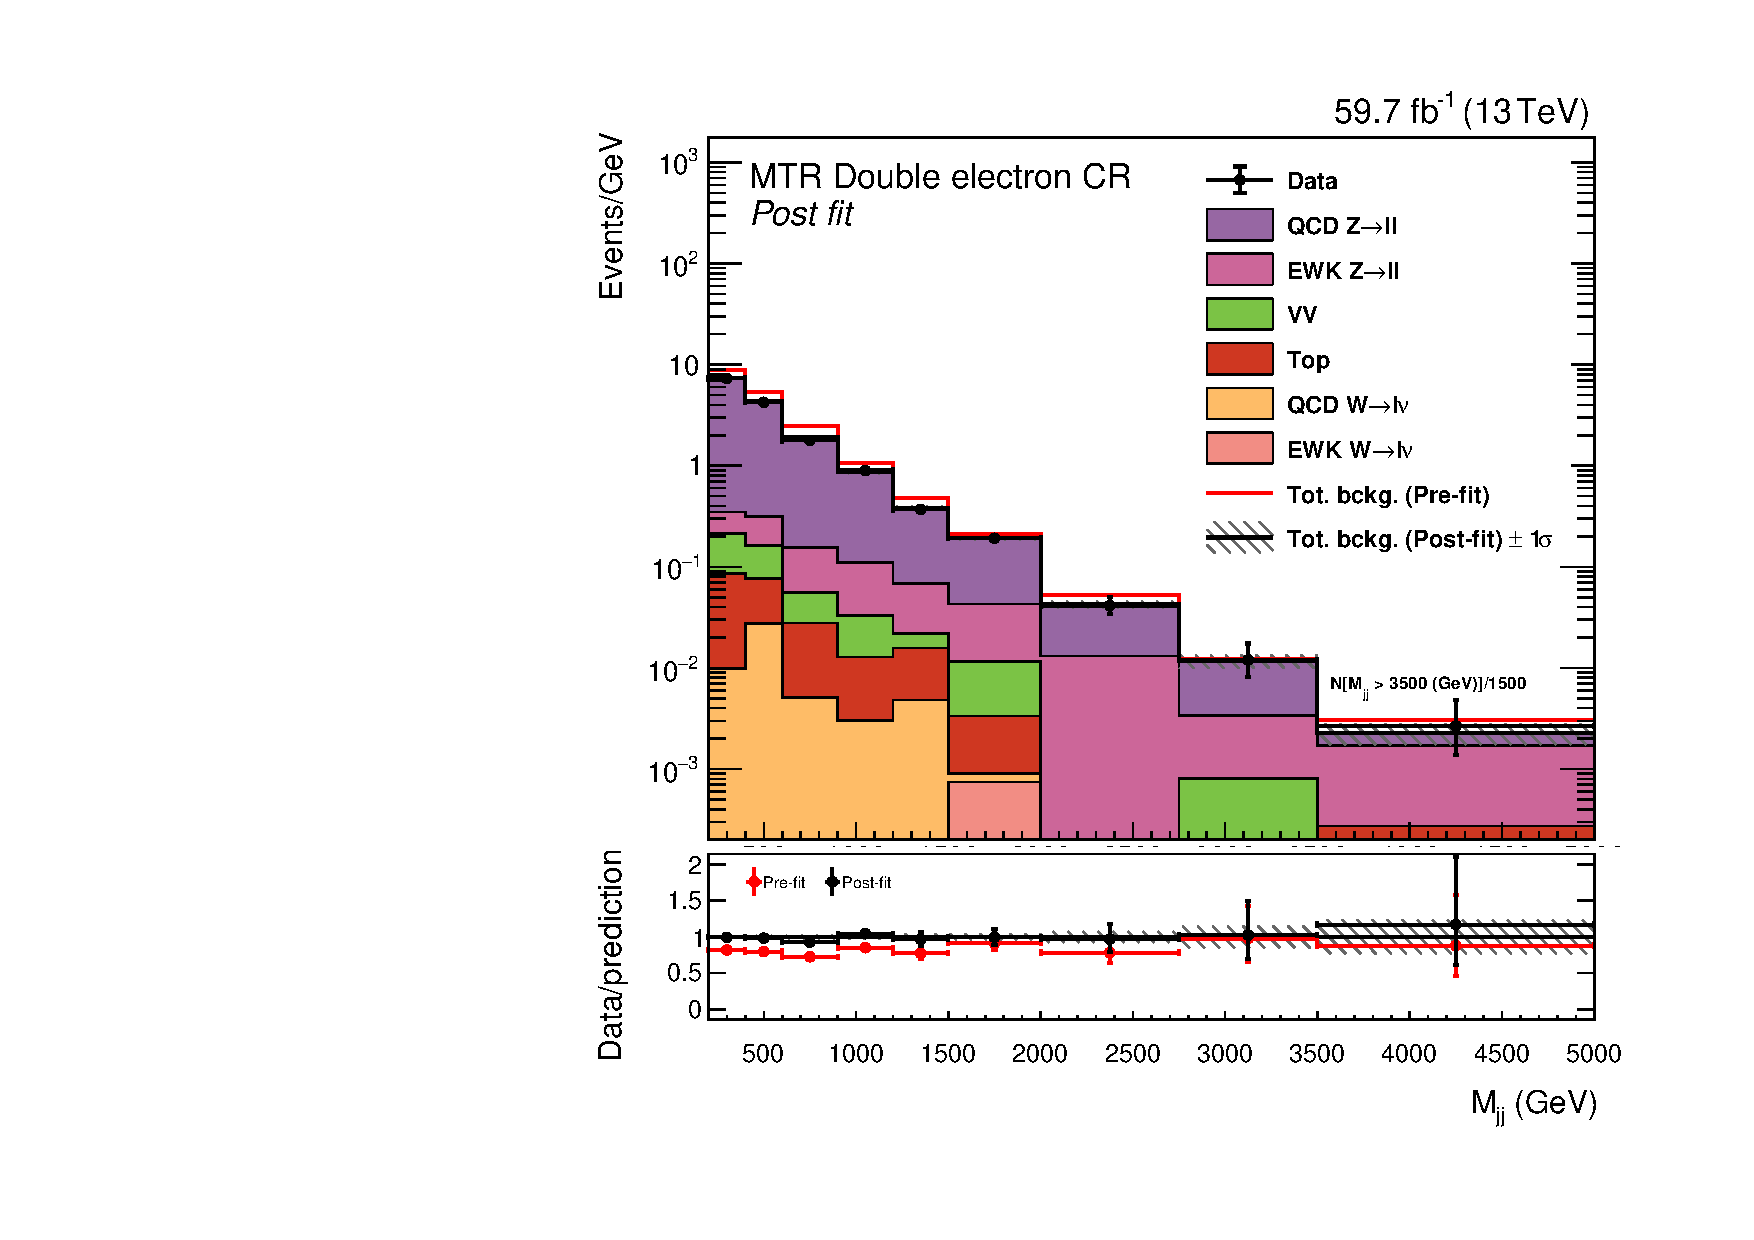
\includegraphics[width= 0.47\textwidth]{Results/SplusBFit/MTR_2018_ZEE.pdf}}\\
     \subfigure[Single muon CR]{ 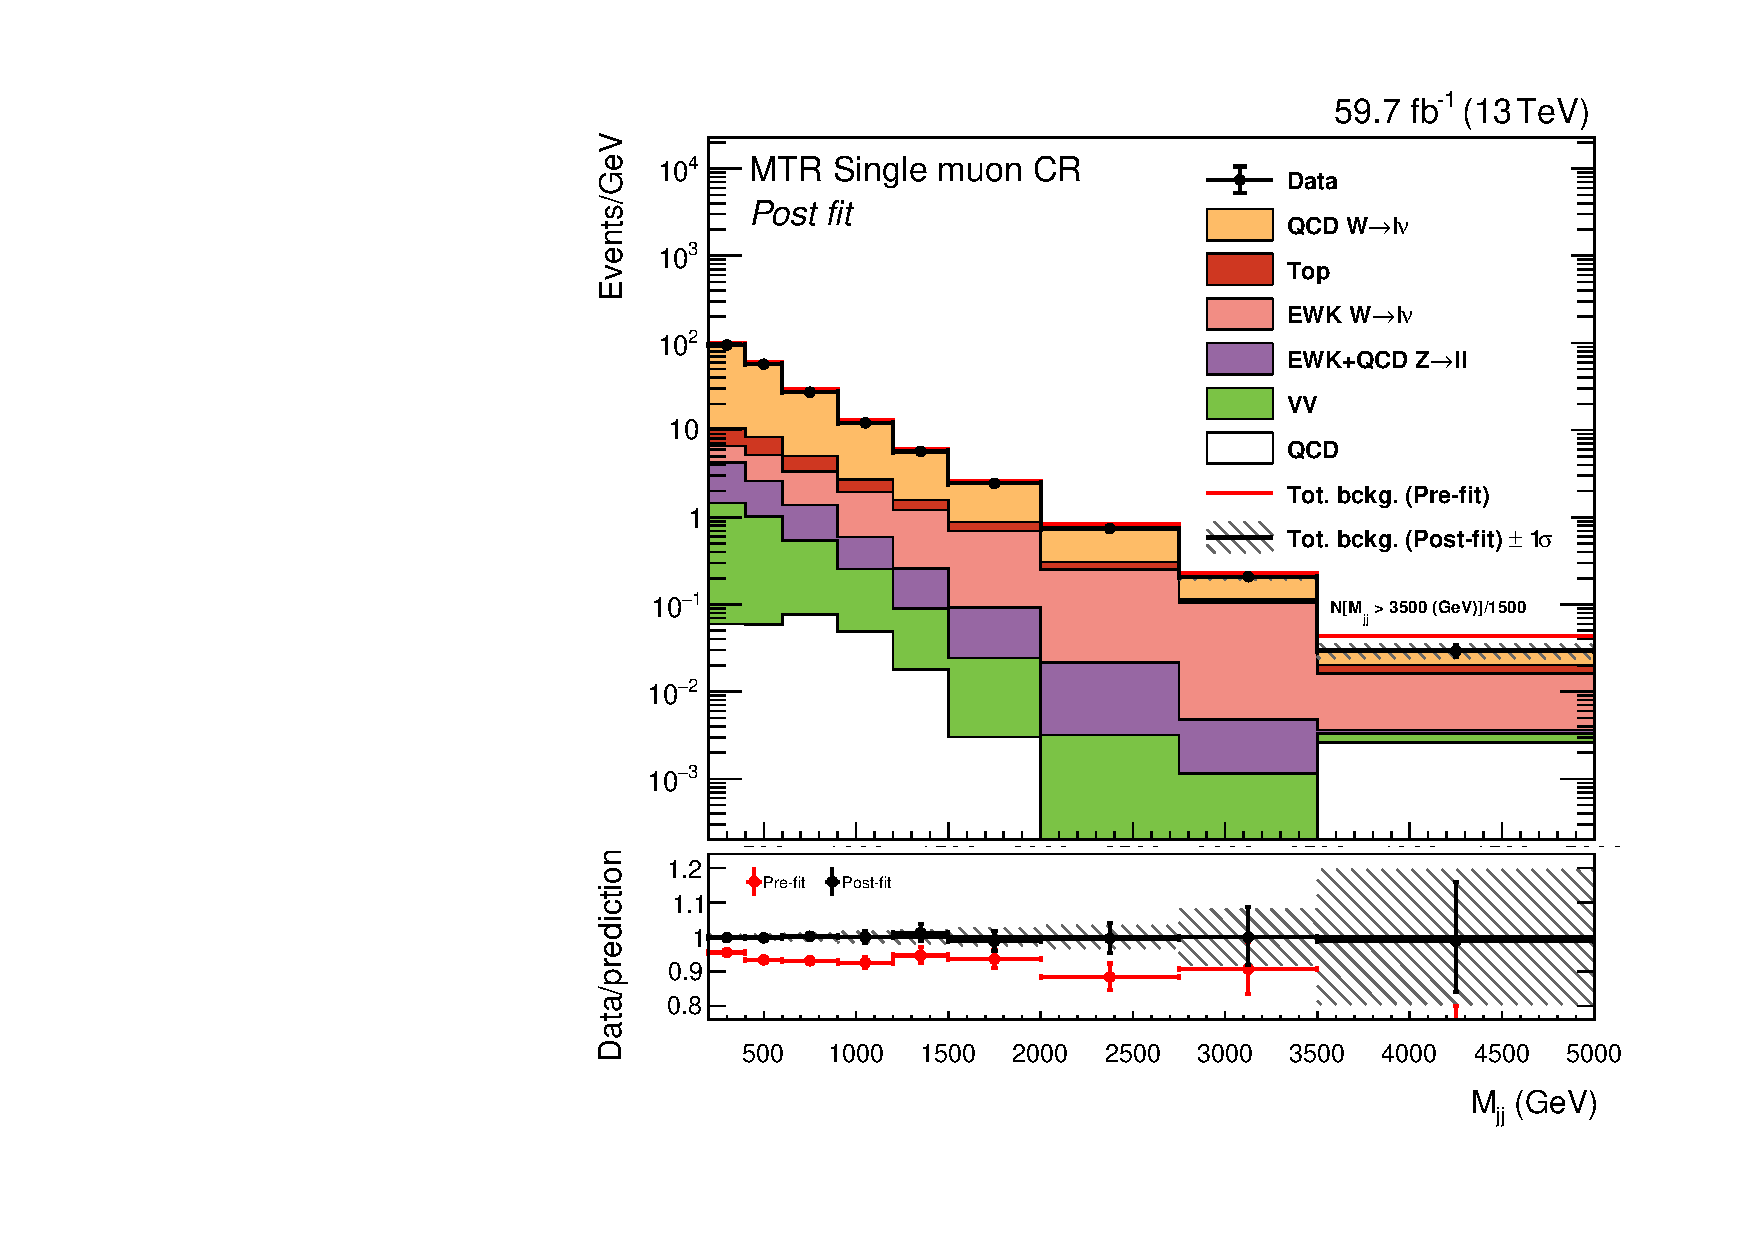
\includegraphics[width= 0.47\textwidth]{Results/SplusBFit/MTR_2018_WMUNU.pdf}}
    \subfigure[Single electron CR]{
    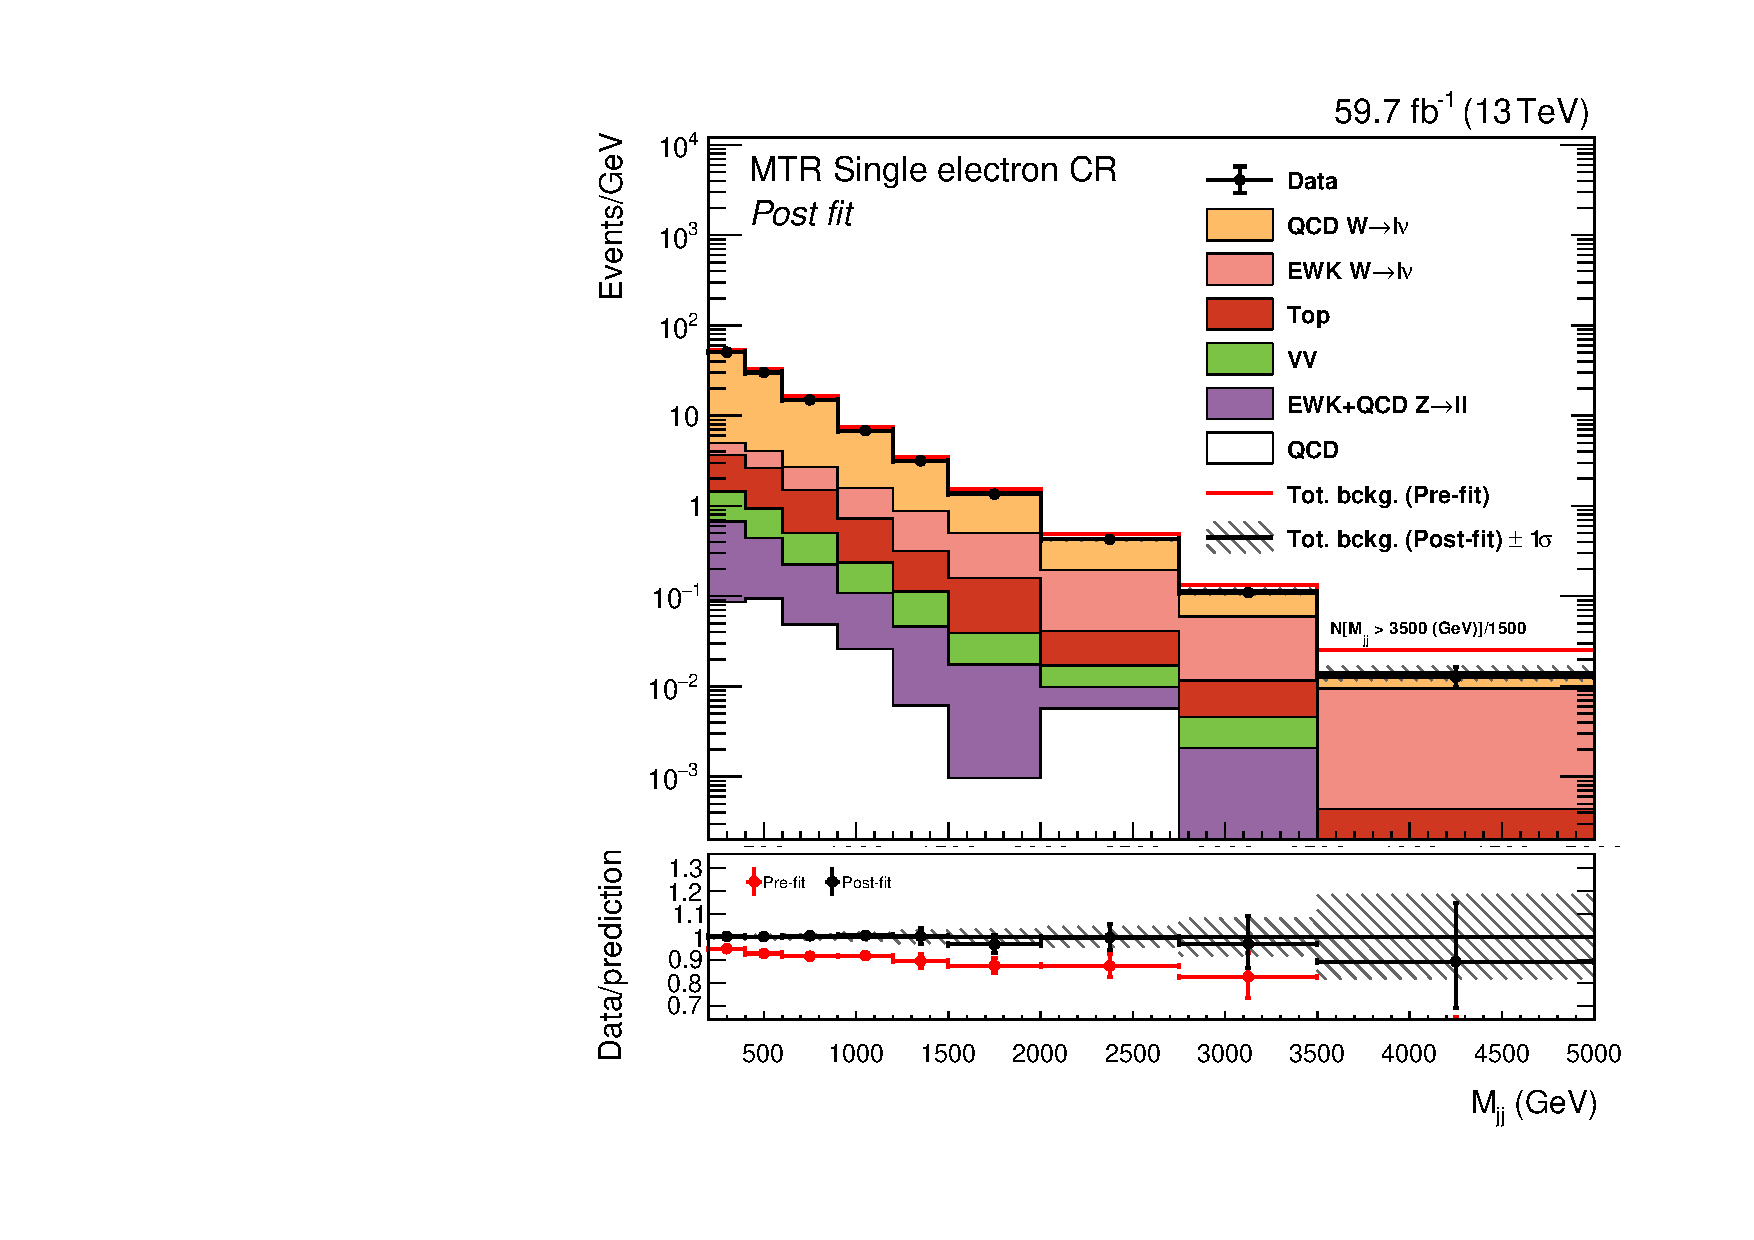
\includegraphics[width= 0.47\textwidth]{Results/SplusBFit/MTR_2018_WENU.pdf}}\\
      \subfigure[Photon CR]{
    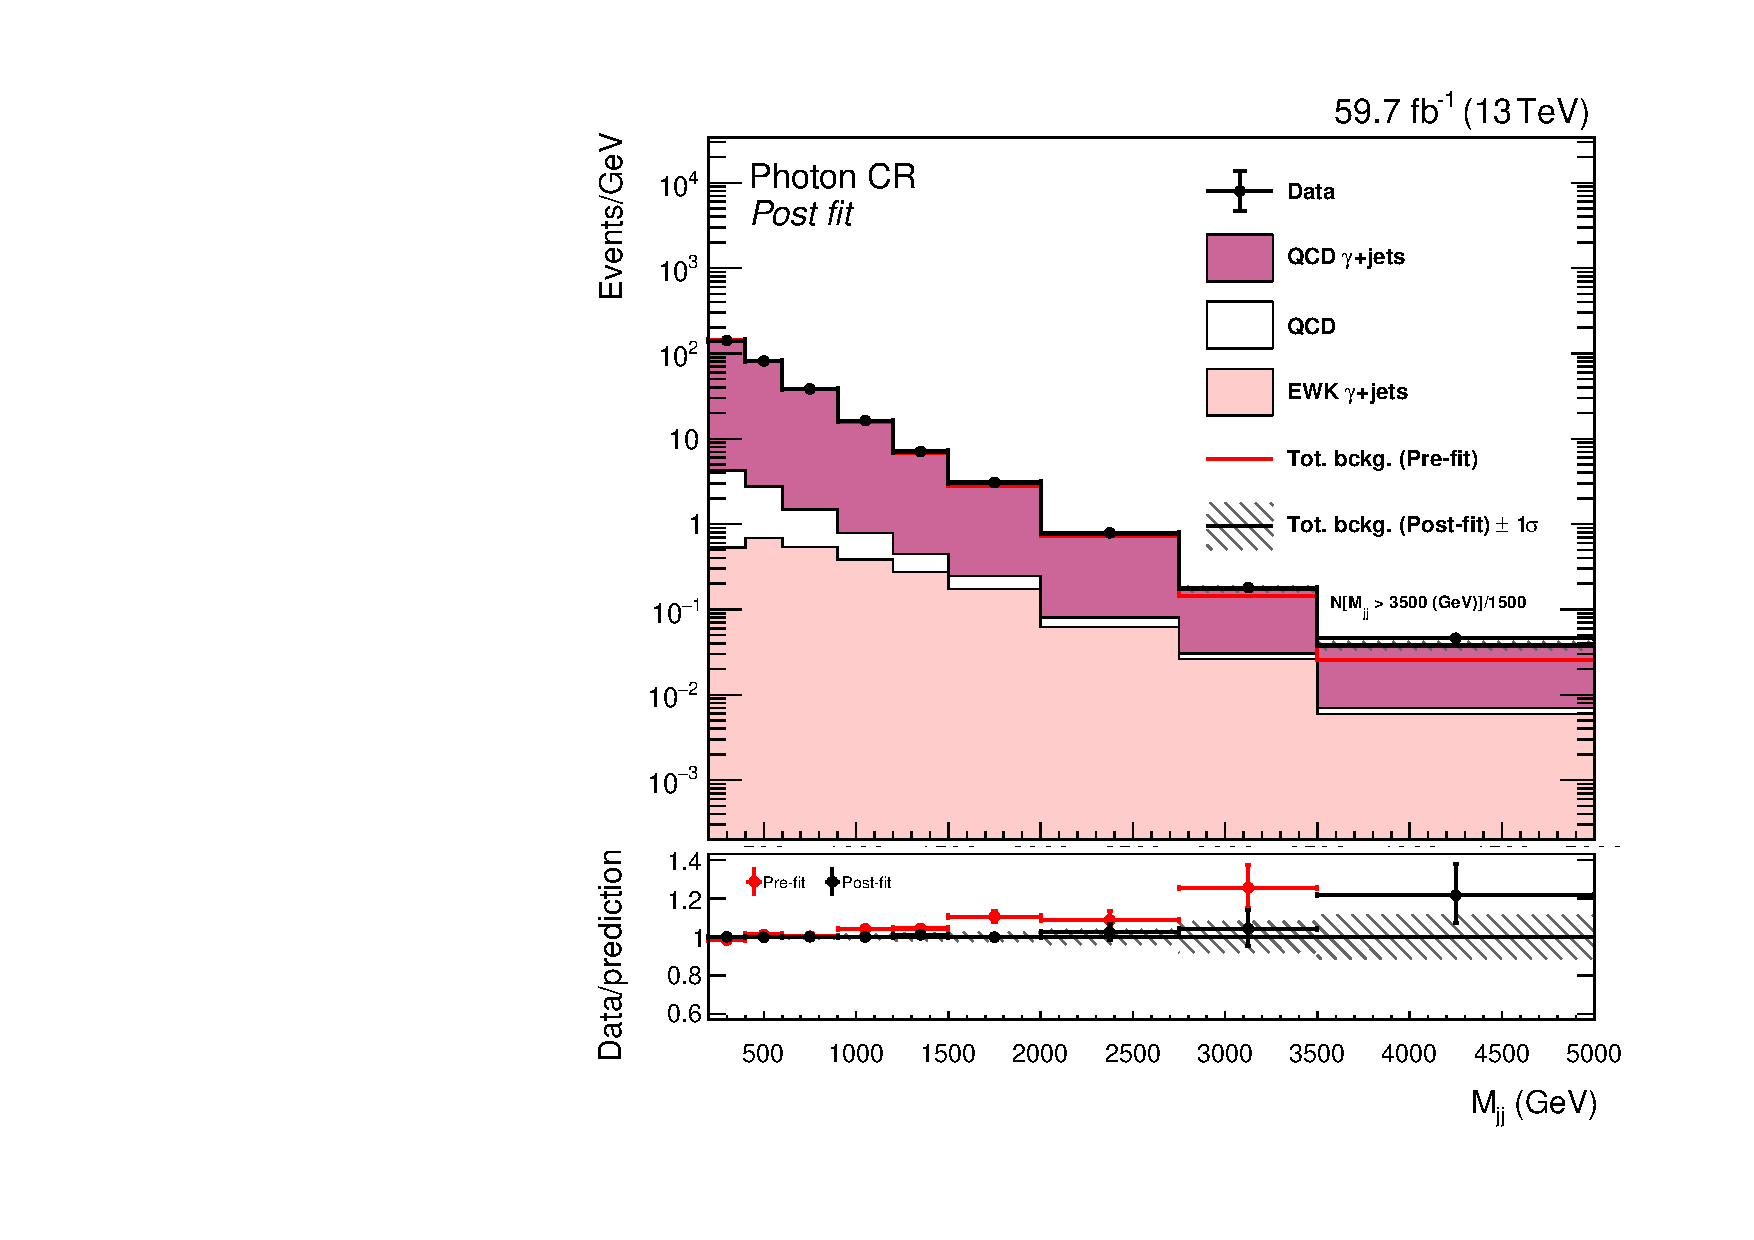
\includegraphics[width= 0.47\textwidth]{Results/SplusBFit/photon_cr_2018.pdf}}
  \caption{Post-fit distributions for 2018 data, showing the: (a) dimuon, (b) dielectron, (c) single muon, (d) single electron and (e) photon CR region.}
  \label{fig:MTR_2018_CR}
\end{figure}


\begin{figure}[htbp]
  \centering
   \subfigure[Dimuon CR]{ 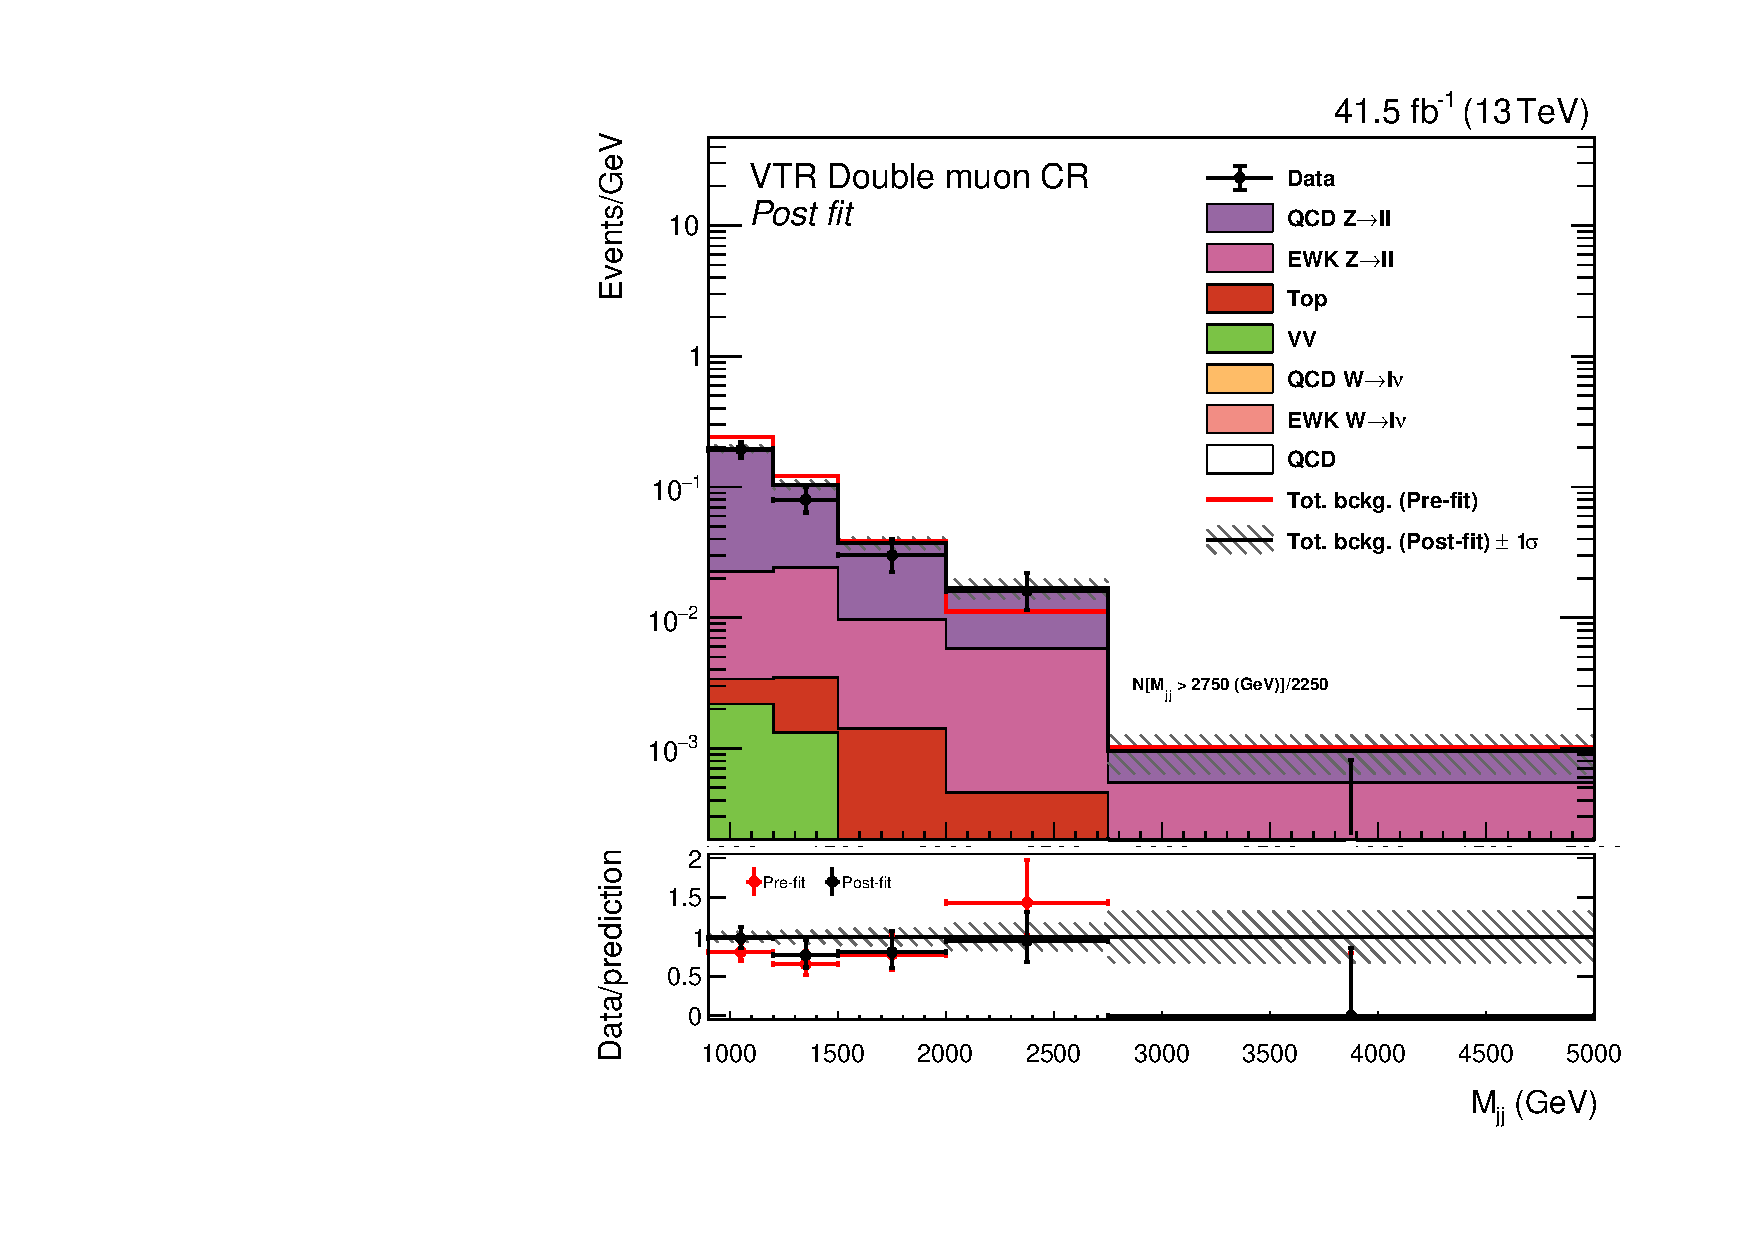
\includegraphics[width= 0.47\textwidth]{Results/SplusBFit/VTR_2017_ZMUMU.pdf}}
     \subfigure[Dielectron CR]{ 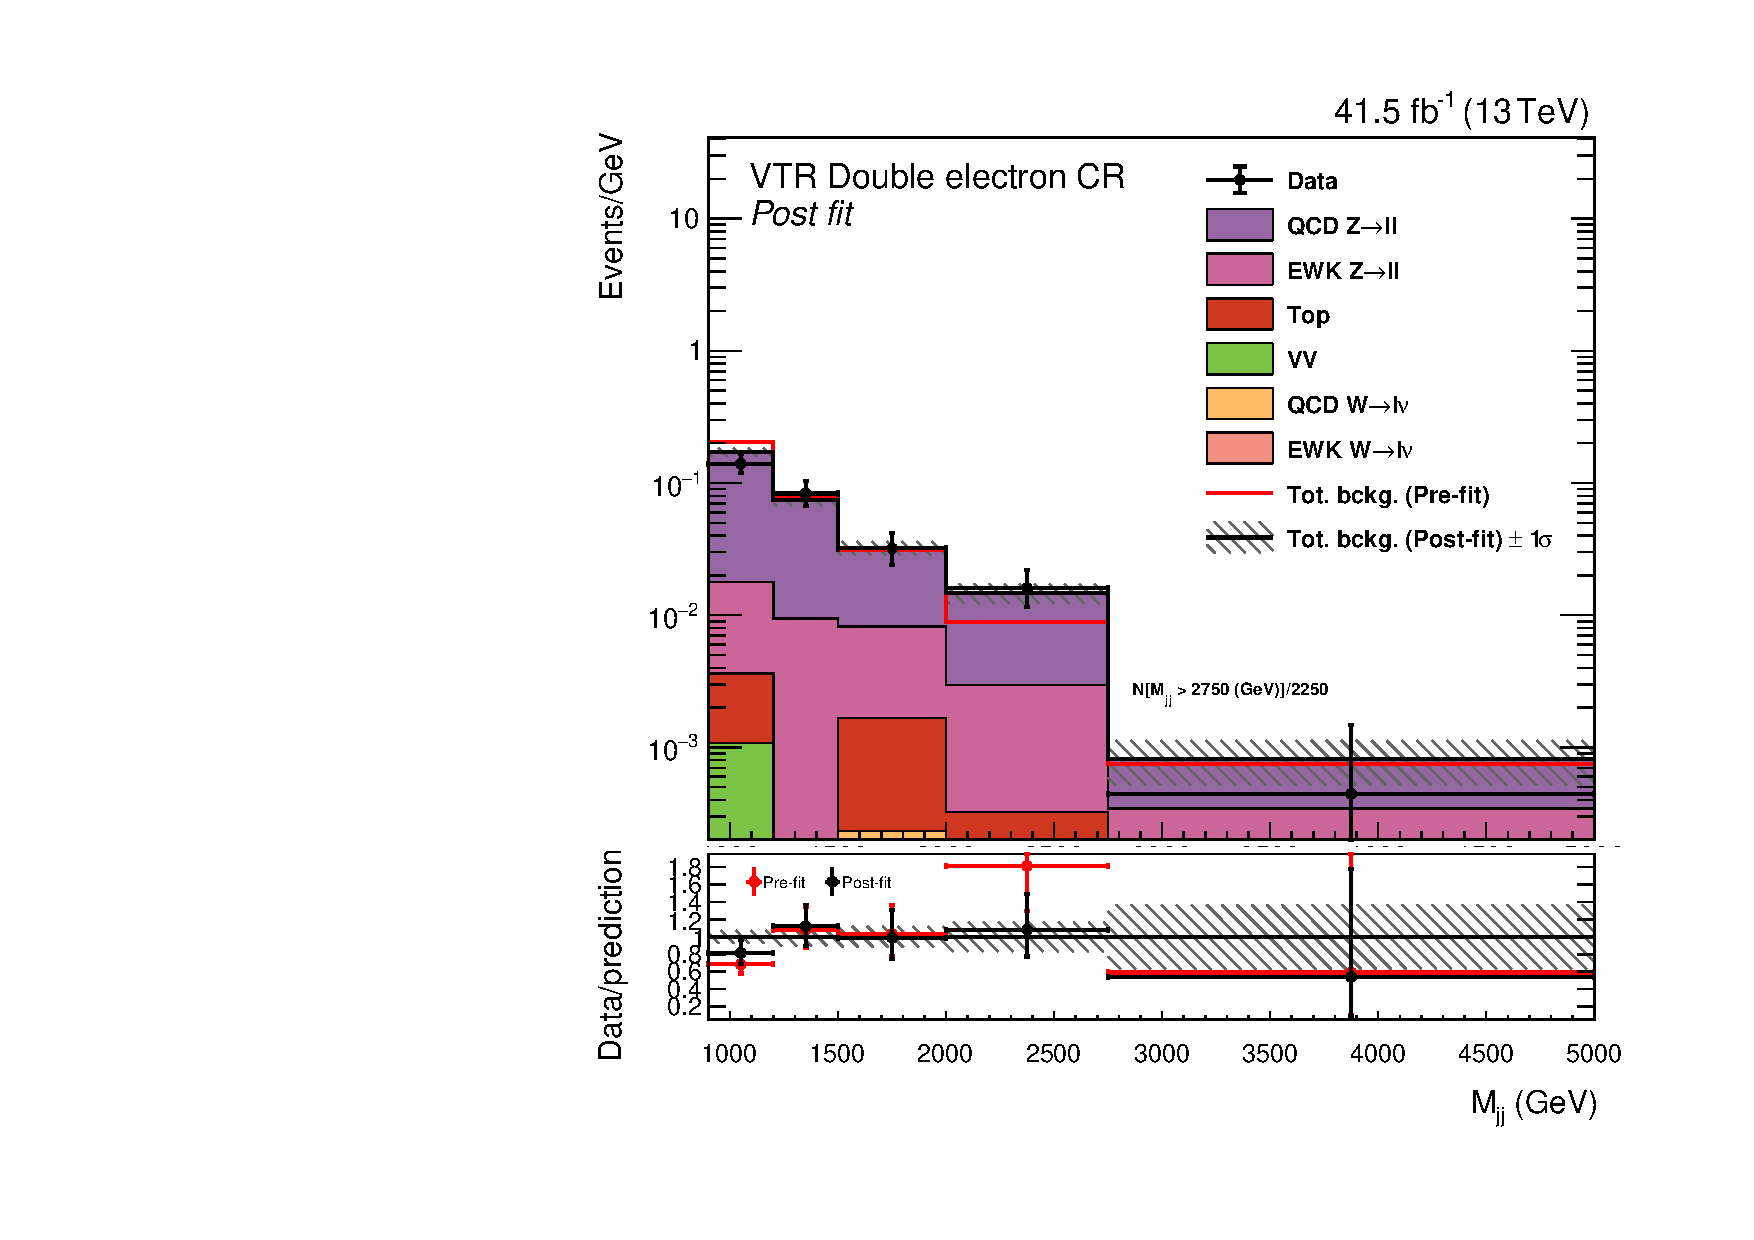
\includegraphics[width= 0.47\textwidth]{Results/SplusBFit/VTR_2017_ZEE.pdf}}\\
     \subfigure[Single muon CR]{ 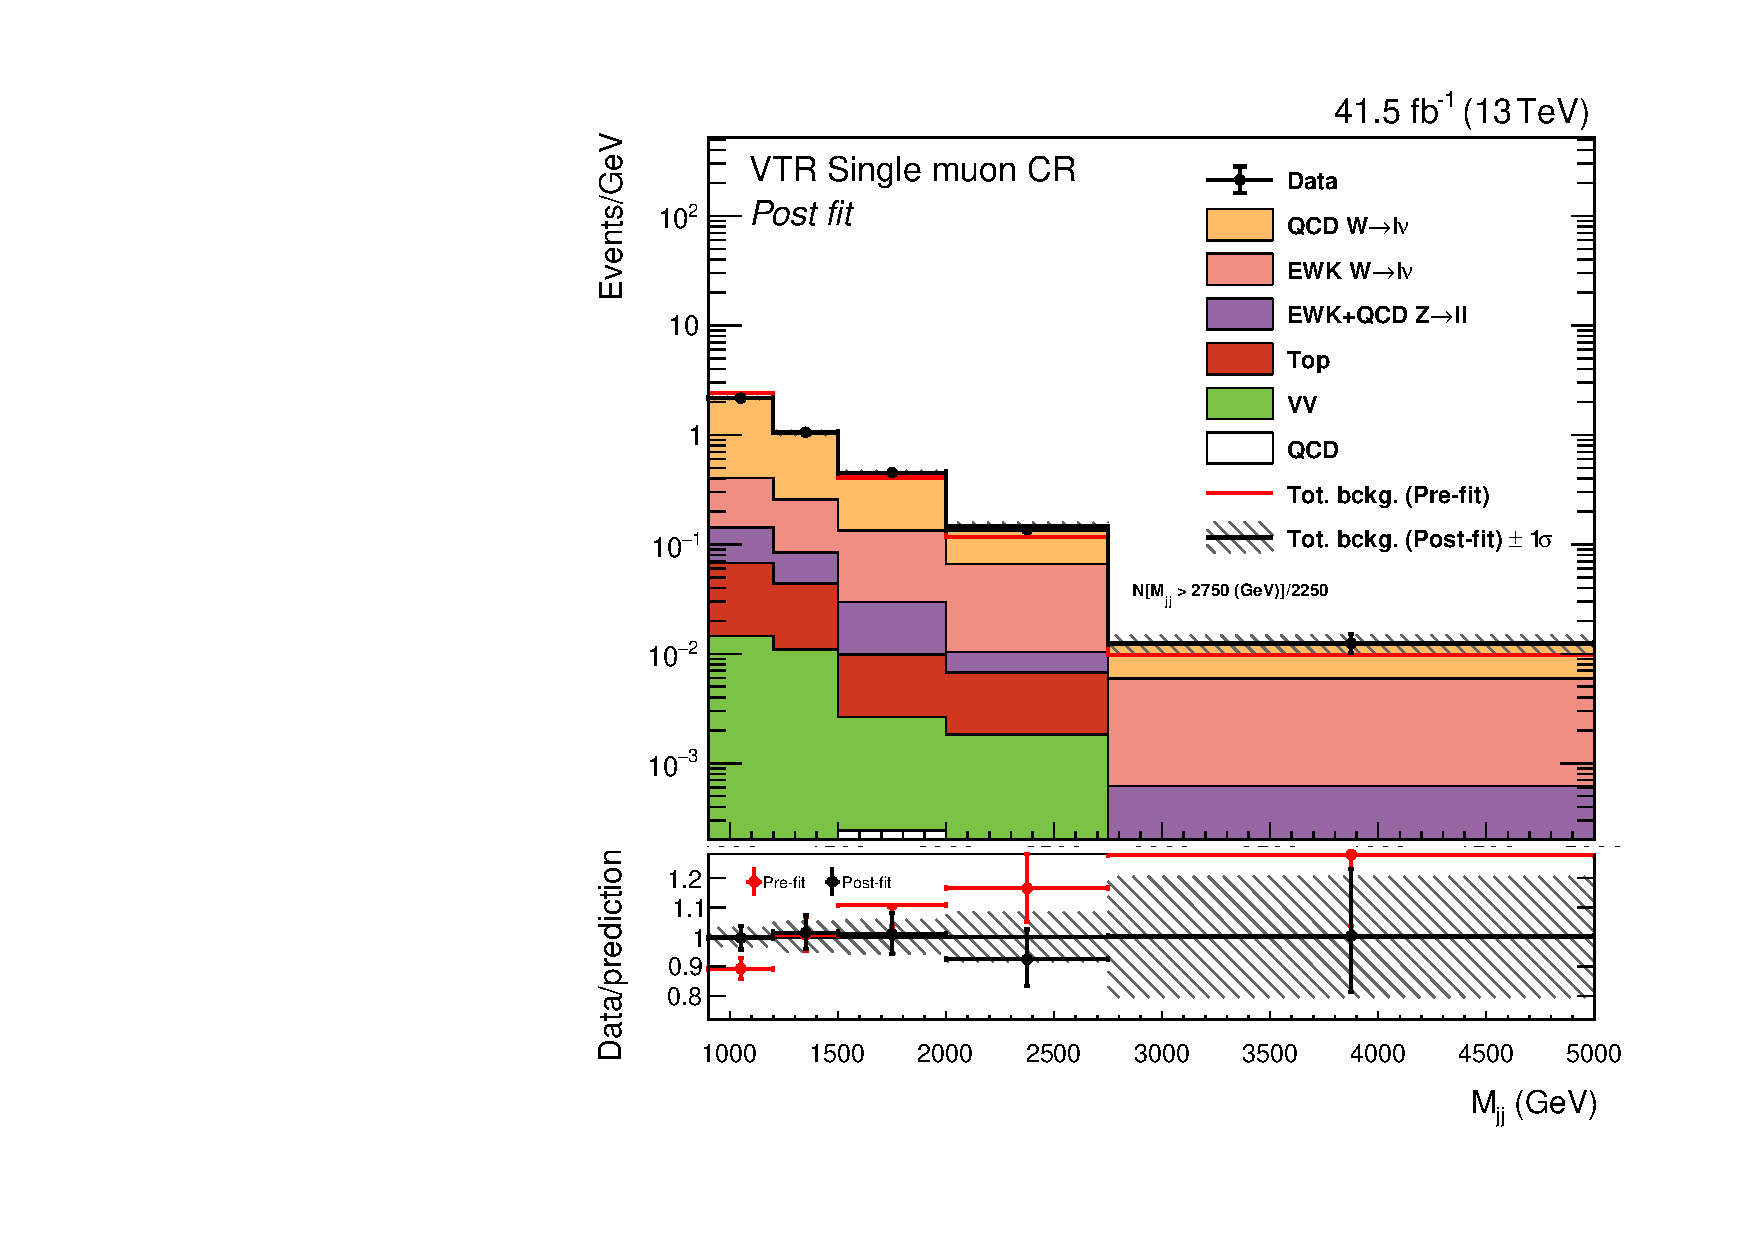
\includegraphics[width= 0.47\textwidth]{Results/SplusBFit/VTR_2017_WMUNU.pdf}}
    \subfigure[Single electron CR]{
    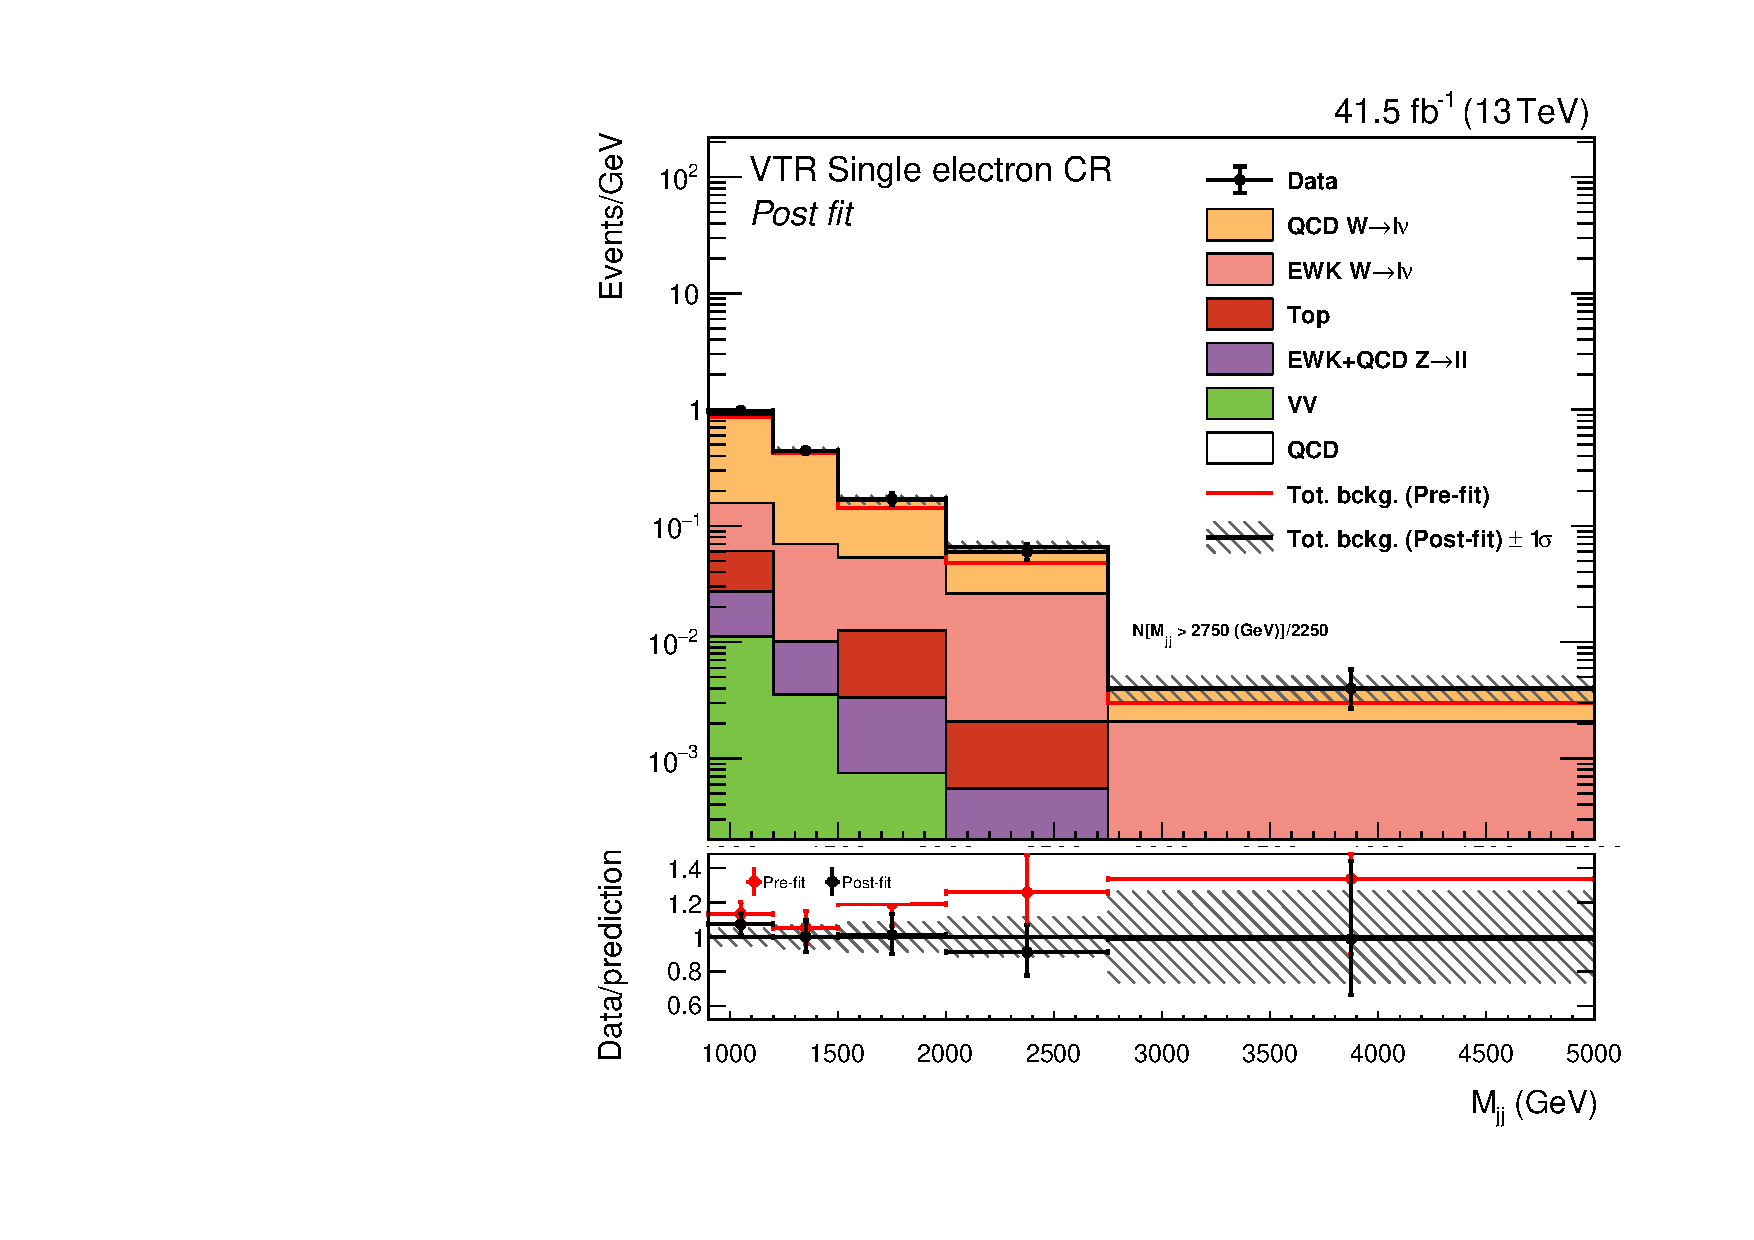
\includegraphics[width= 0.47\textwidth]{Results/SplusBFit/VTR_2017_WENU.pdf}}
  \caption{Post-fit distributions for 2017 data, showing the: (a) dimuon, (b) dielectron, (c) single muon an (d) single electron region.}
  \label{fig:VTR_2017_CR}
\end{figure}

\begin{figure}[htbp]
  \centering
   \subfigure[Dimuon CR]{ 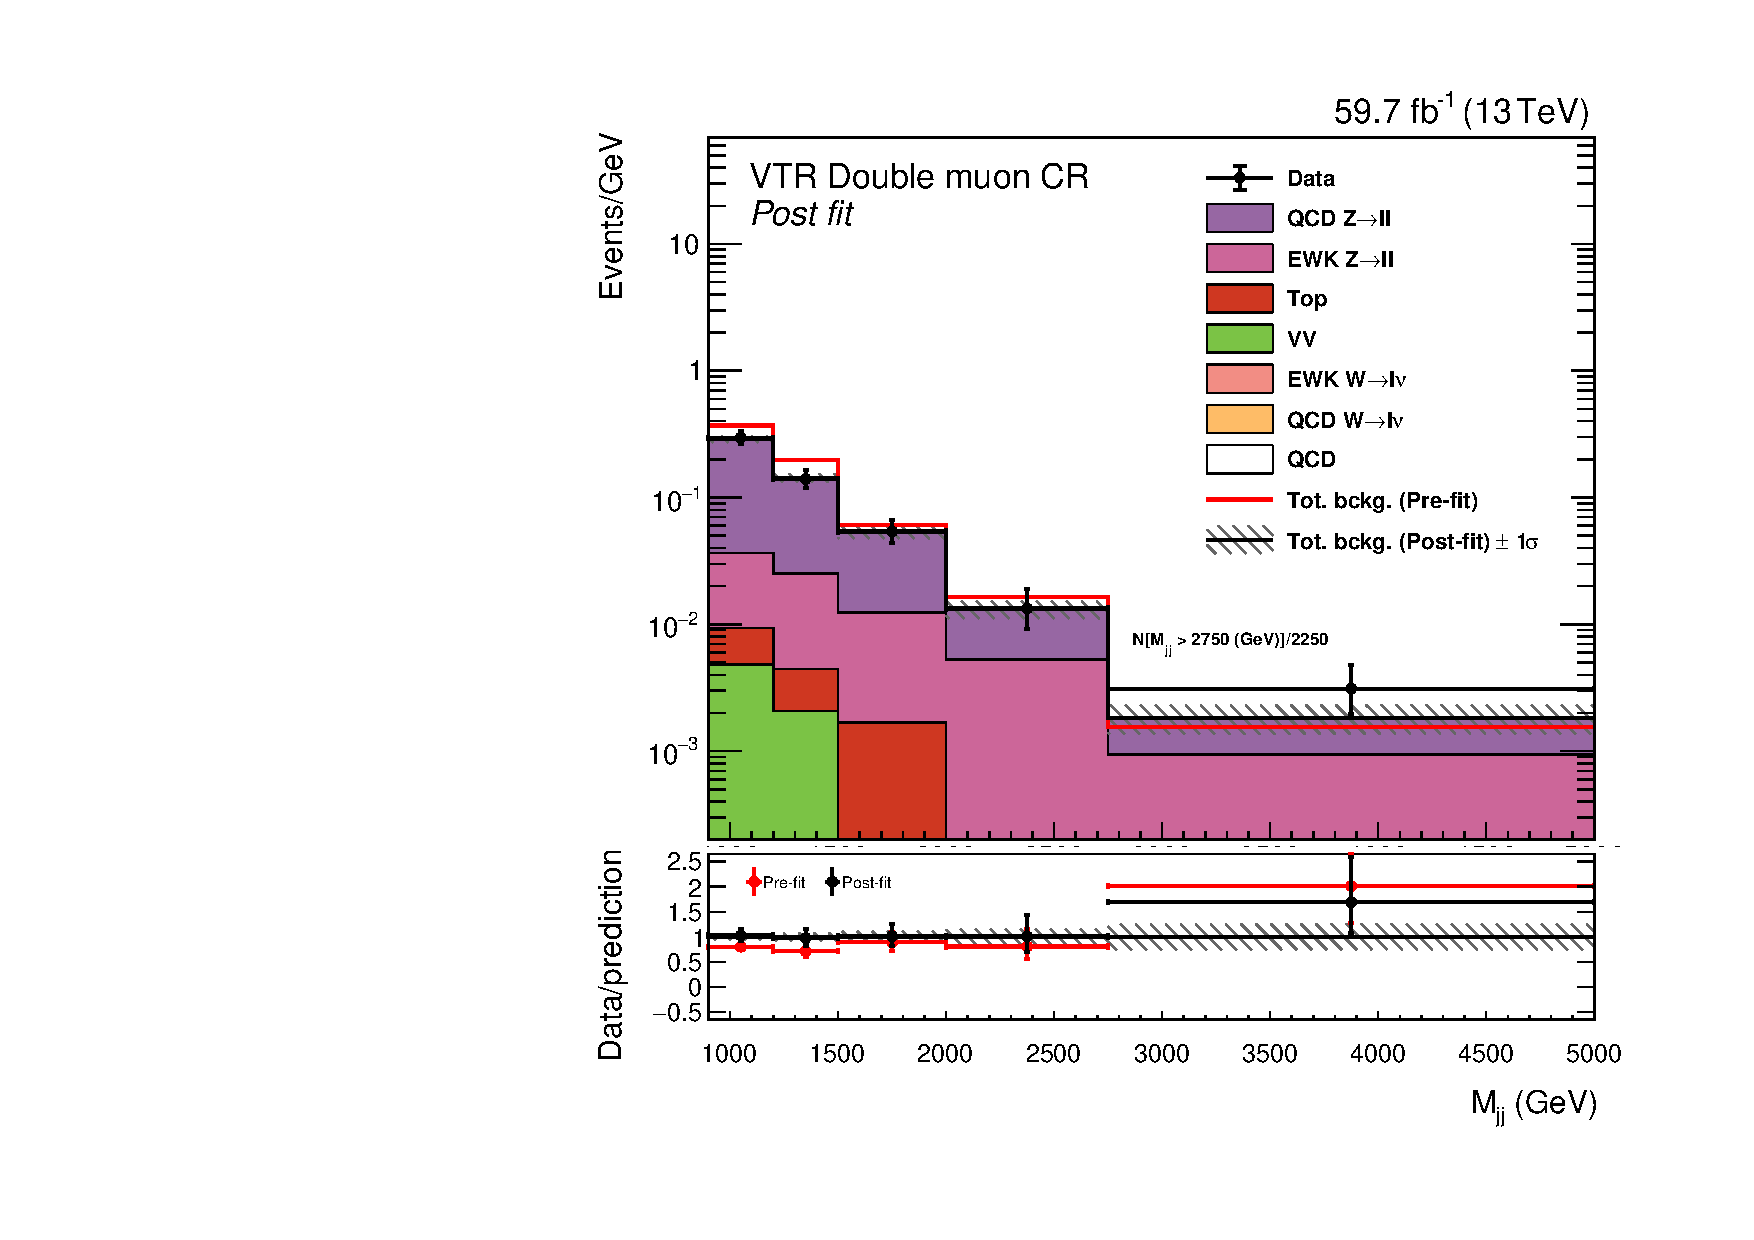
\includegraphics[width= 0.47\textwidth]{Results/SplusBFit/VTR_2018_ZMUMU.pdf}}
     \subfigure[Dielectron CR]{ 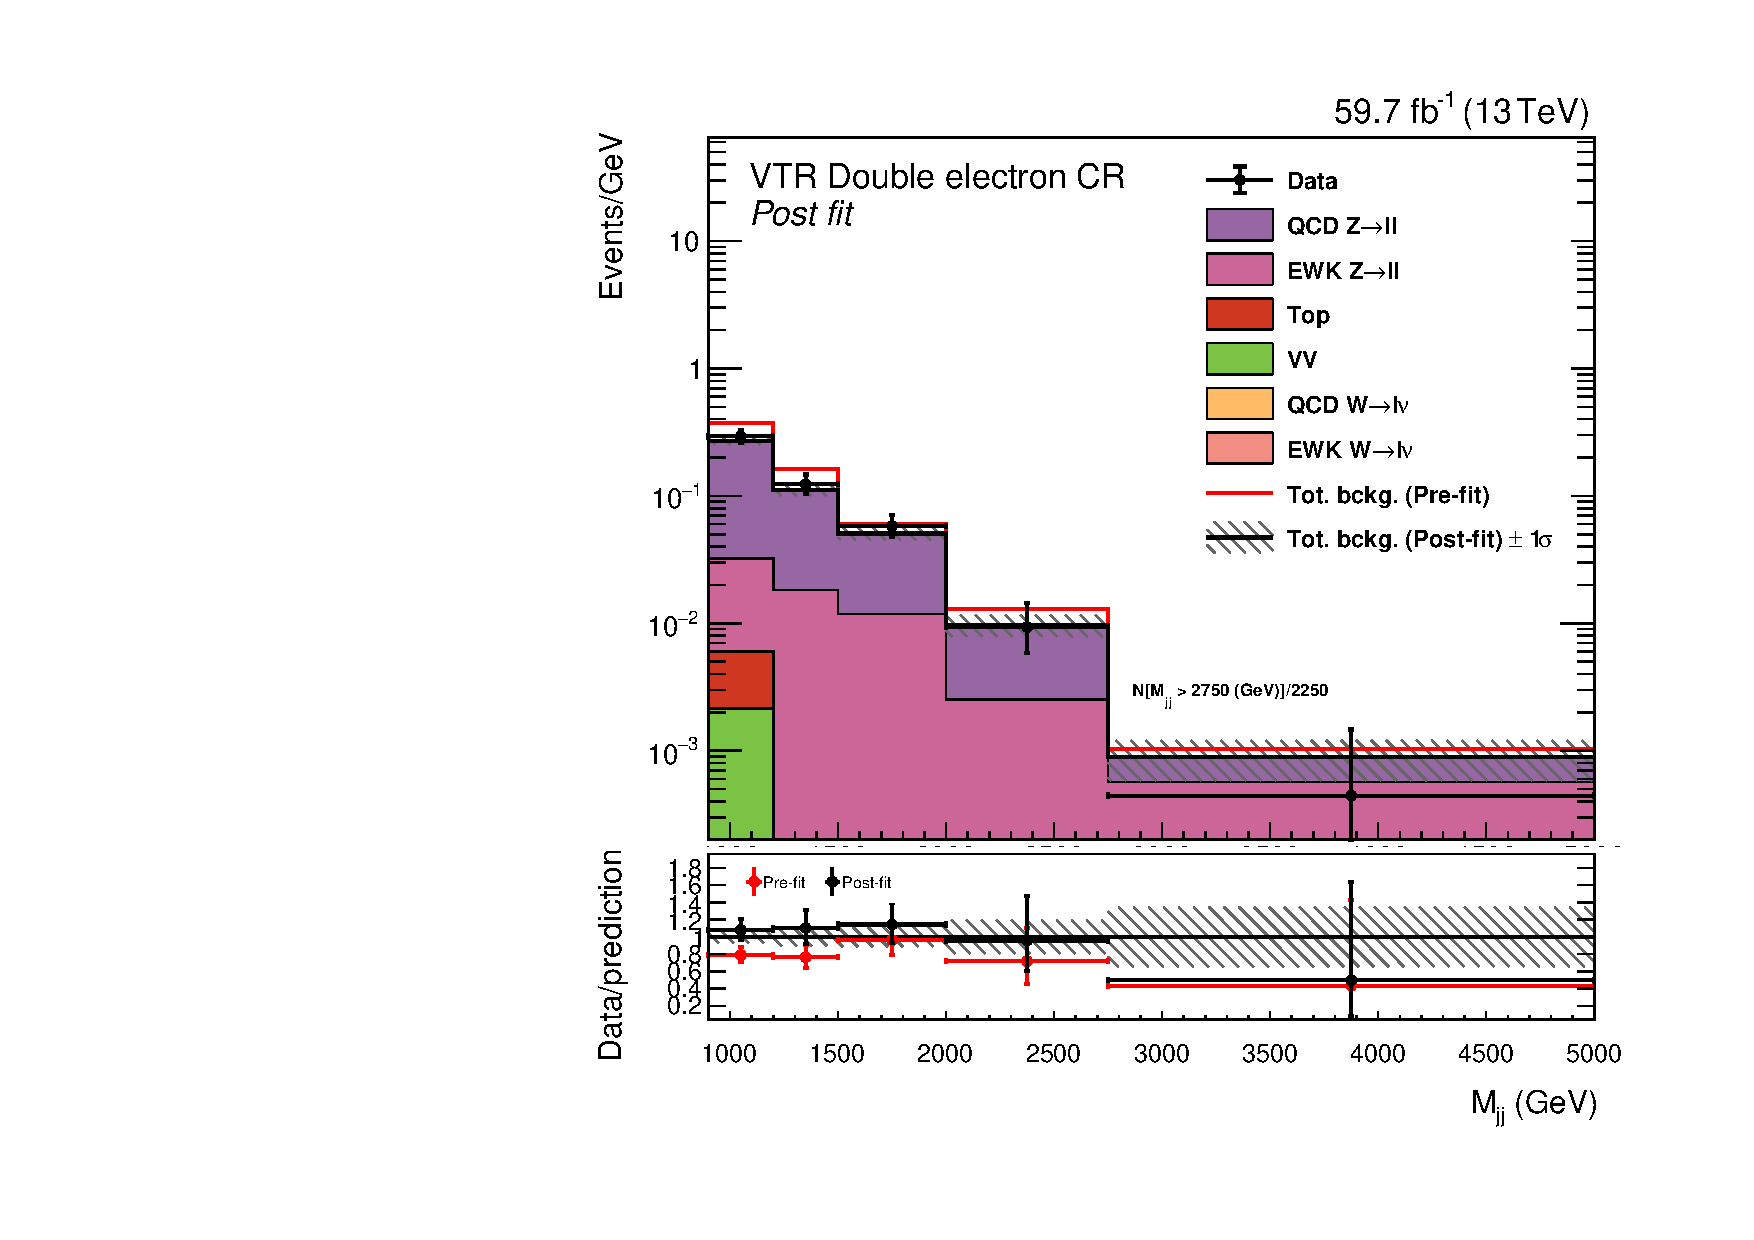
\includegraphics[width= 0.47\textwidth]{Results/SplusBFit/VTR_2018_ZEE.pdf}}\\
     \subfigure[Single muon CR]{ 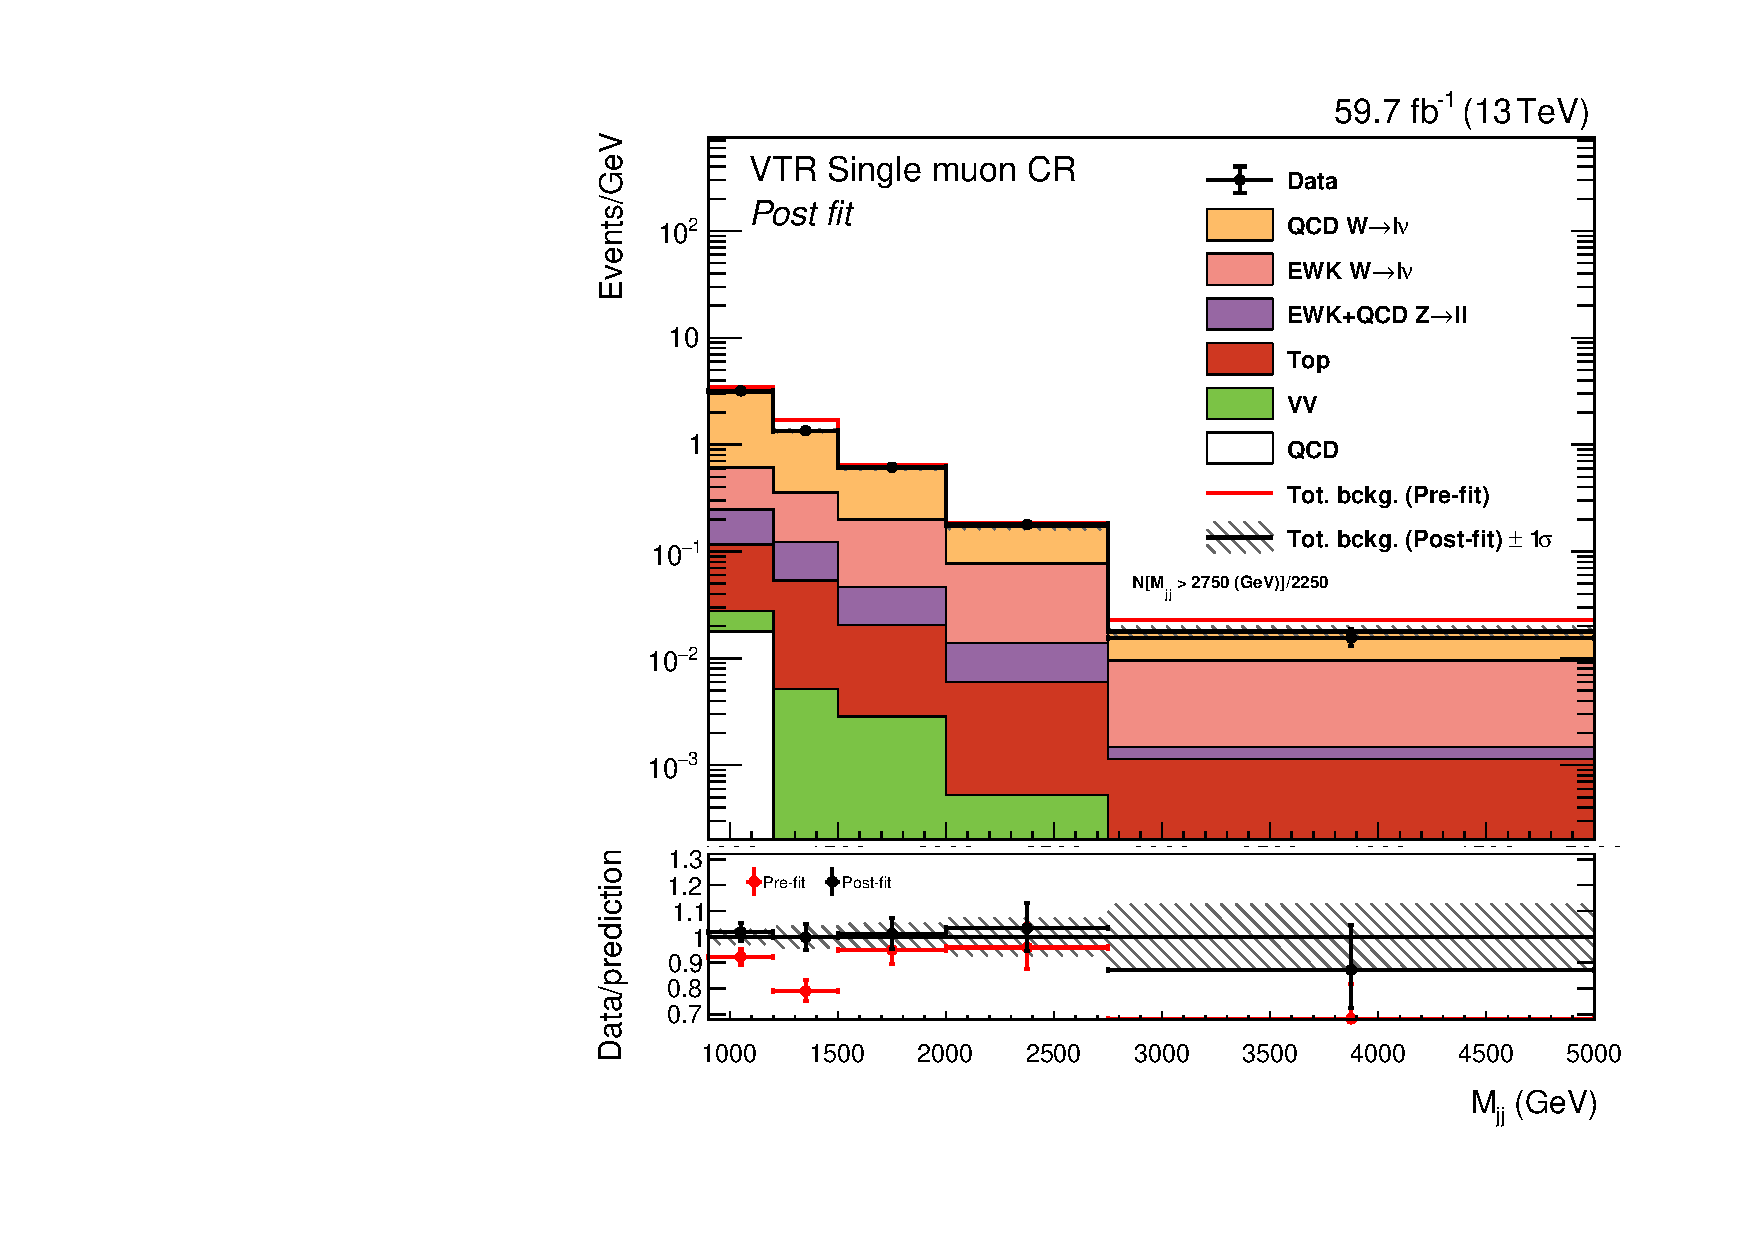
\includegraphics[width= 0.47\textwidth]{Results/SplusBFit/VTR_2018_WMUNU.pdf}}
    \subfigure[Single electron CR]{
    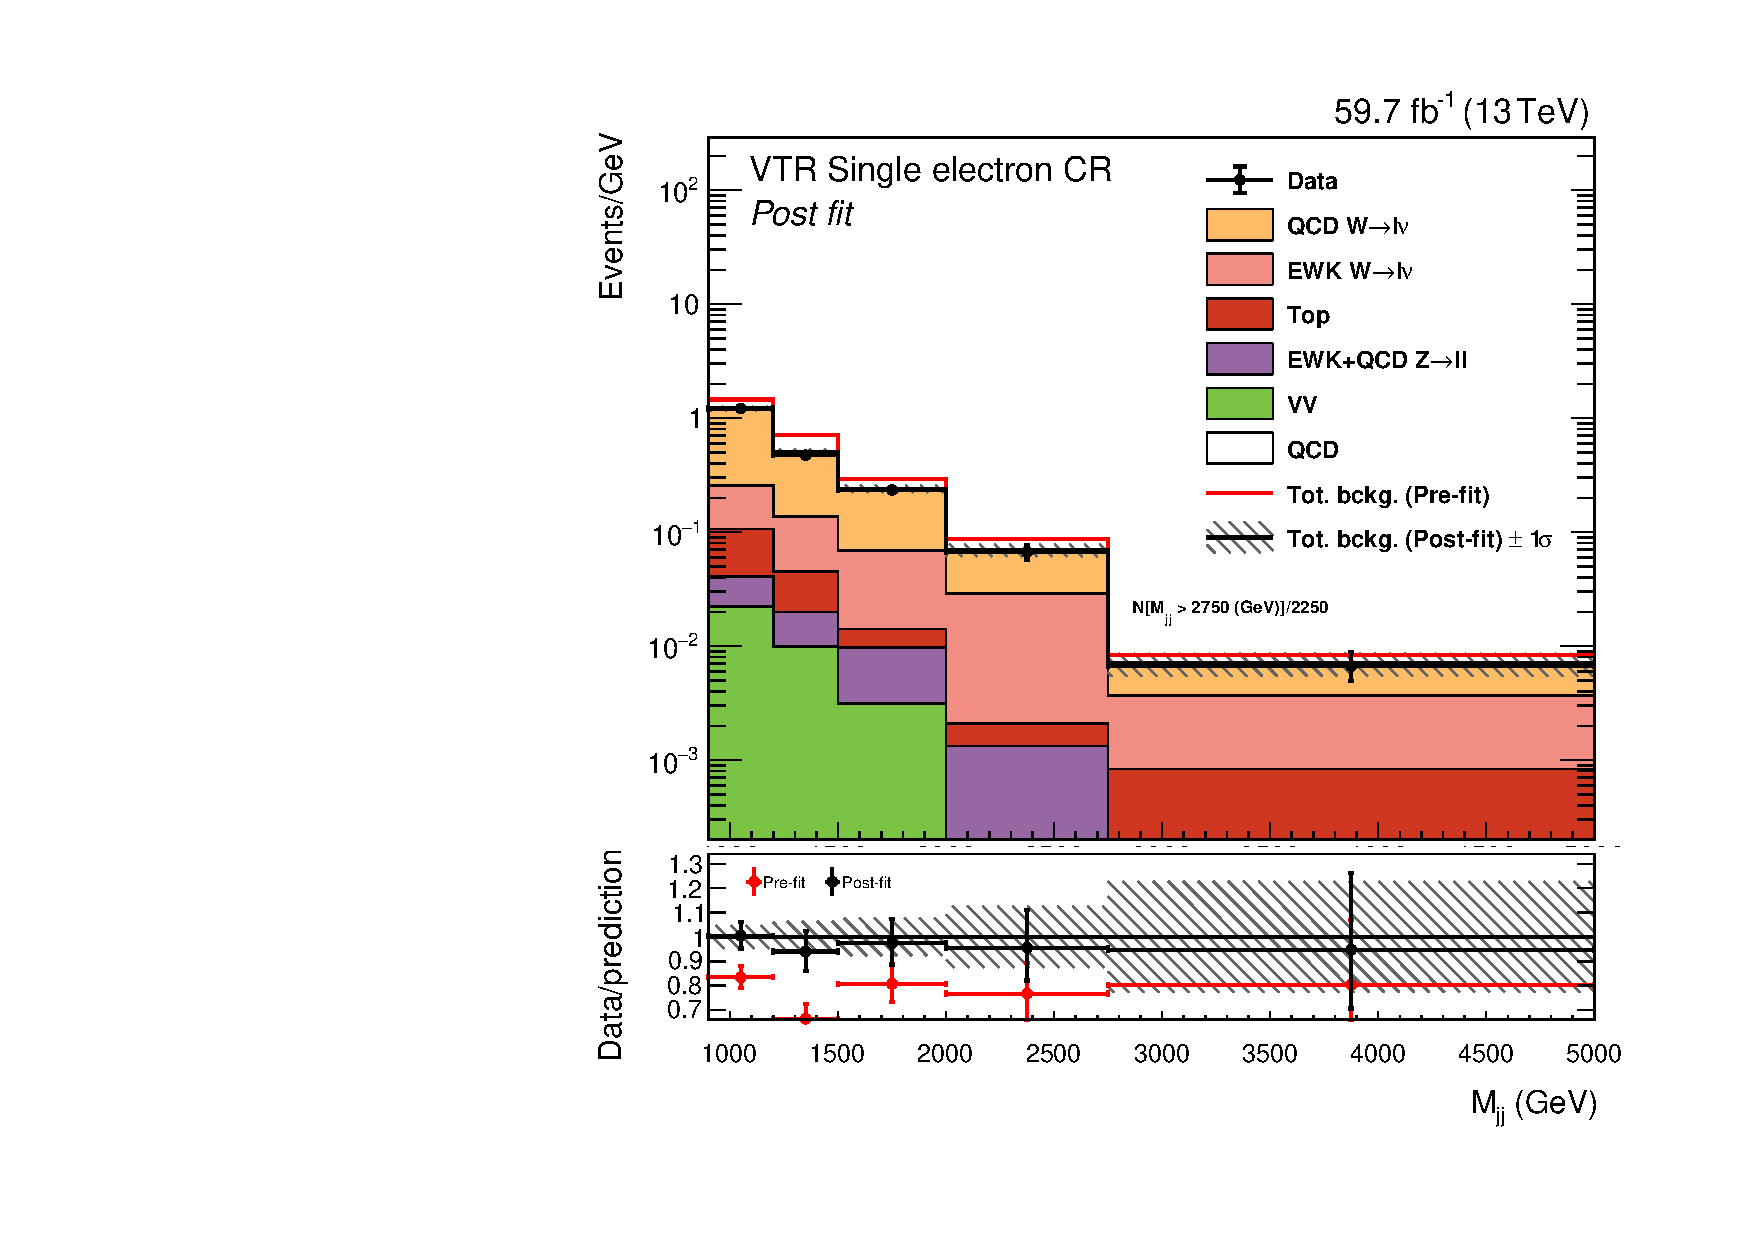
\includegraphics[width= 0.47\textwidth]{Results/SplusBFit/VTR_2018_WENU.pdf}}
  \caption{Post-fit distributions for 2018 data, showing the: (a) dimuon, (b) dielectron, (c) single muon an (d) single electron region.}
  \label{fig:VTR_2018_CR}
\end{figure}


\begin{figure}[htbp]
  \centering
   \subfigure[MTR 2017]{ 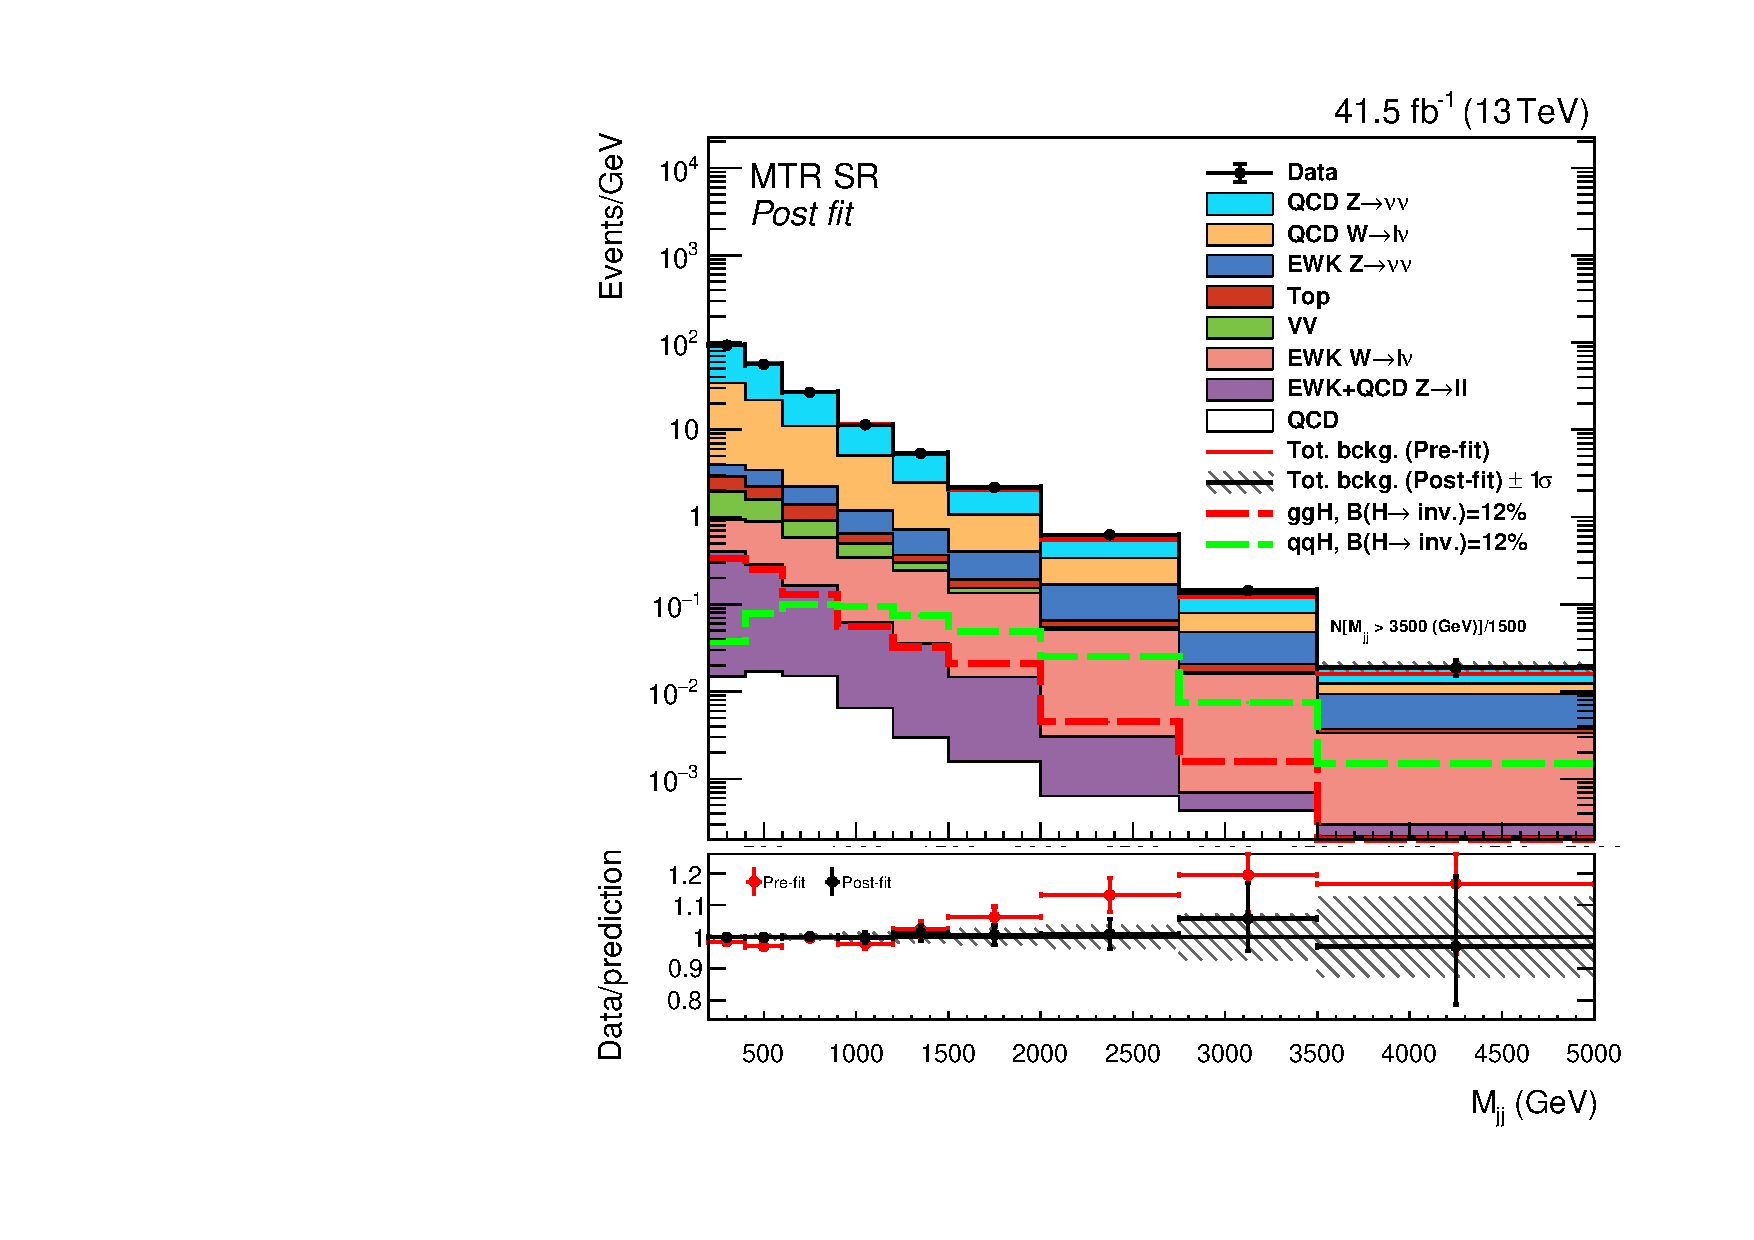
\includegraphics[width= 0.47\textwidth]{Results/SplusBFit/MTR_2017_SR.pdf}}
     \subfigure[MTR 2018]{ 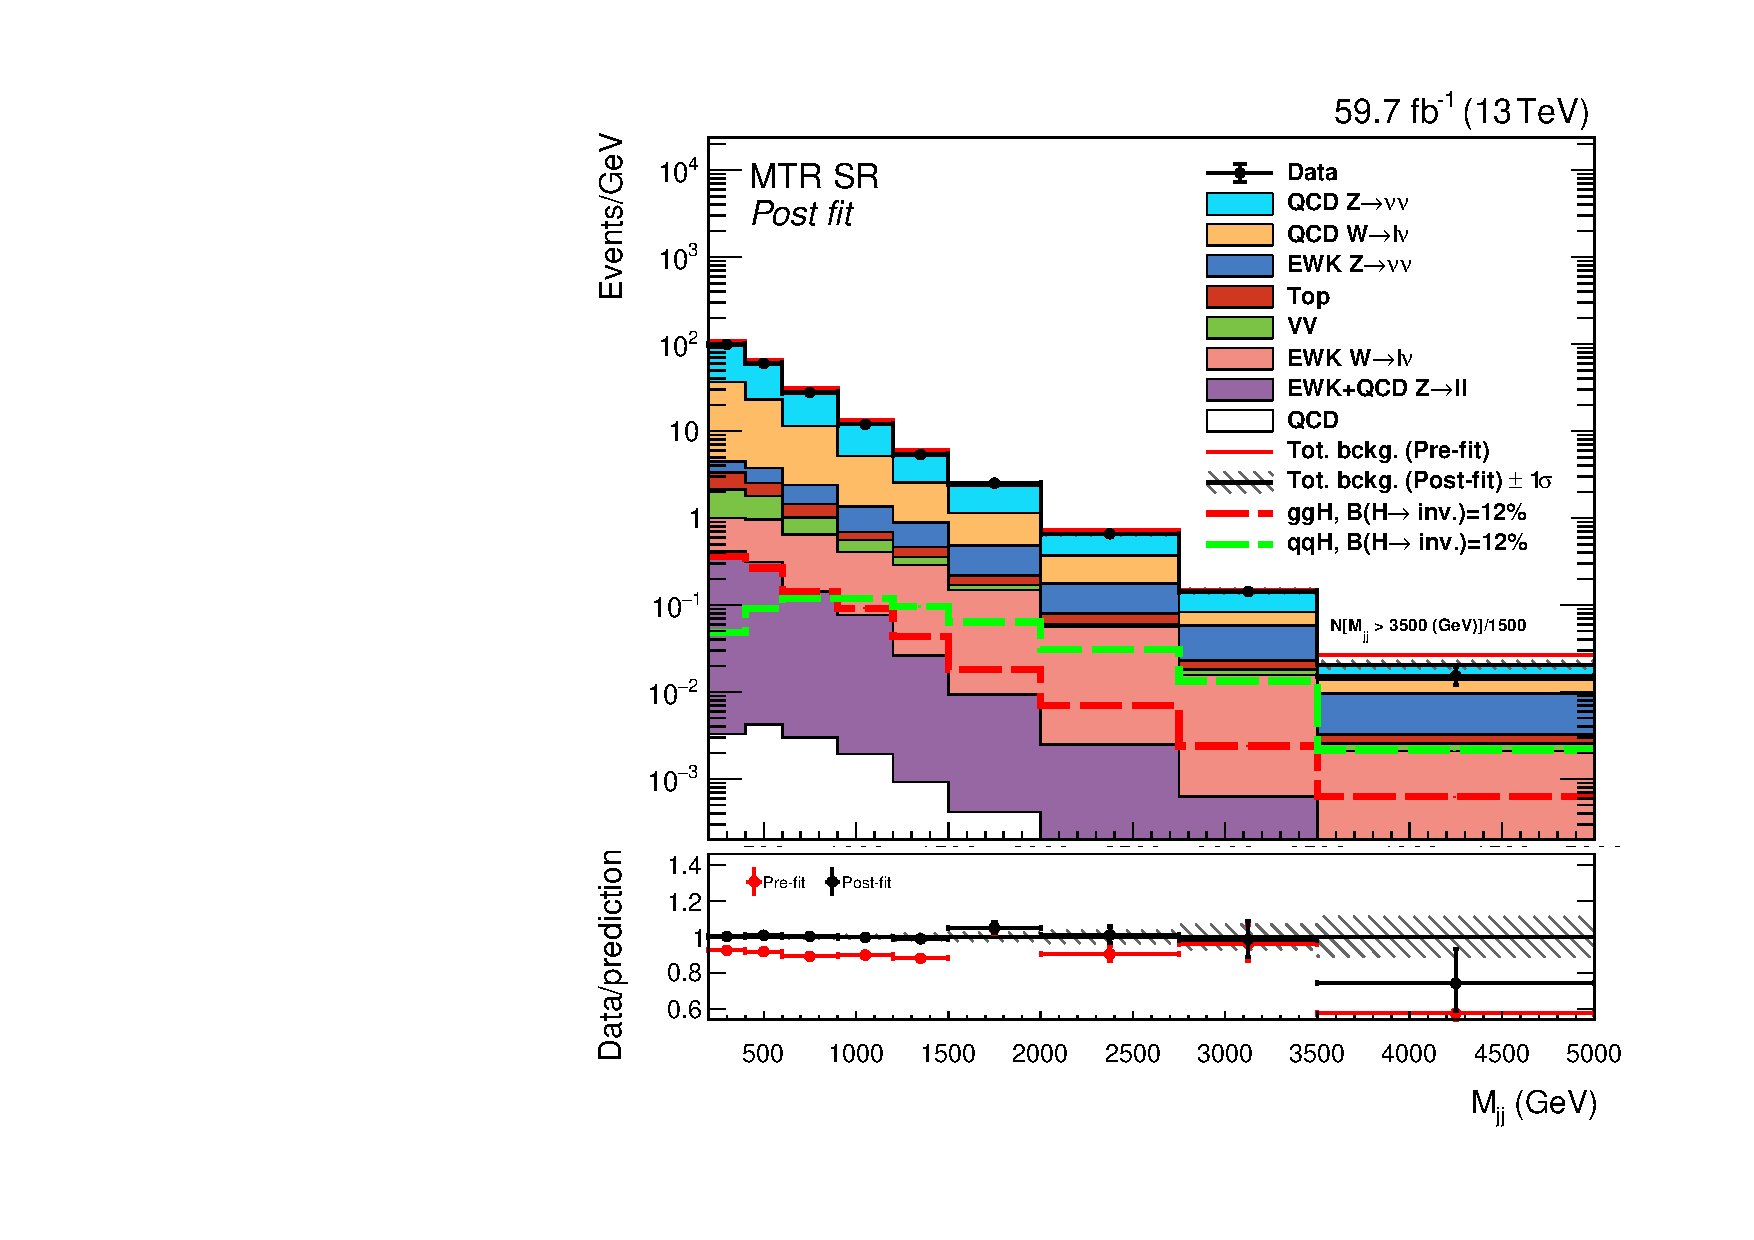
\includegraphics[width= 0.47\textwidth]{Results/SplusBFit/MTR_2018_SR.pdf}}\\
     \subfigure[VTR 2017]{ 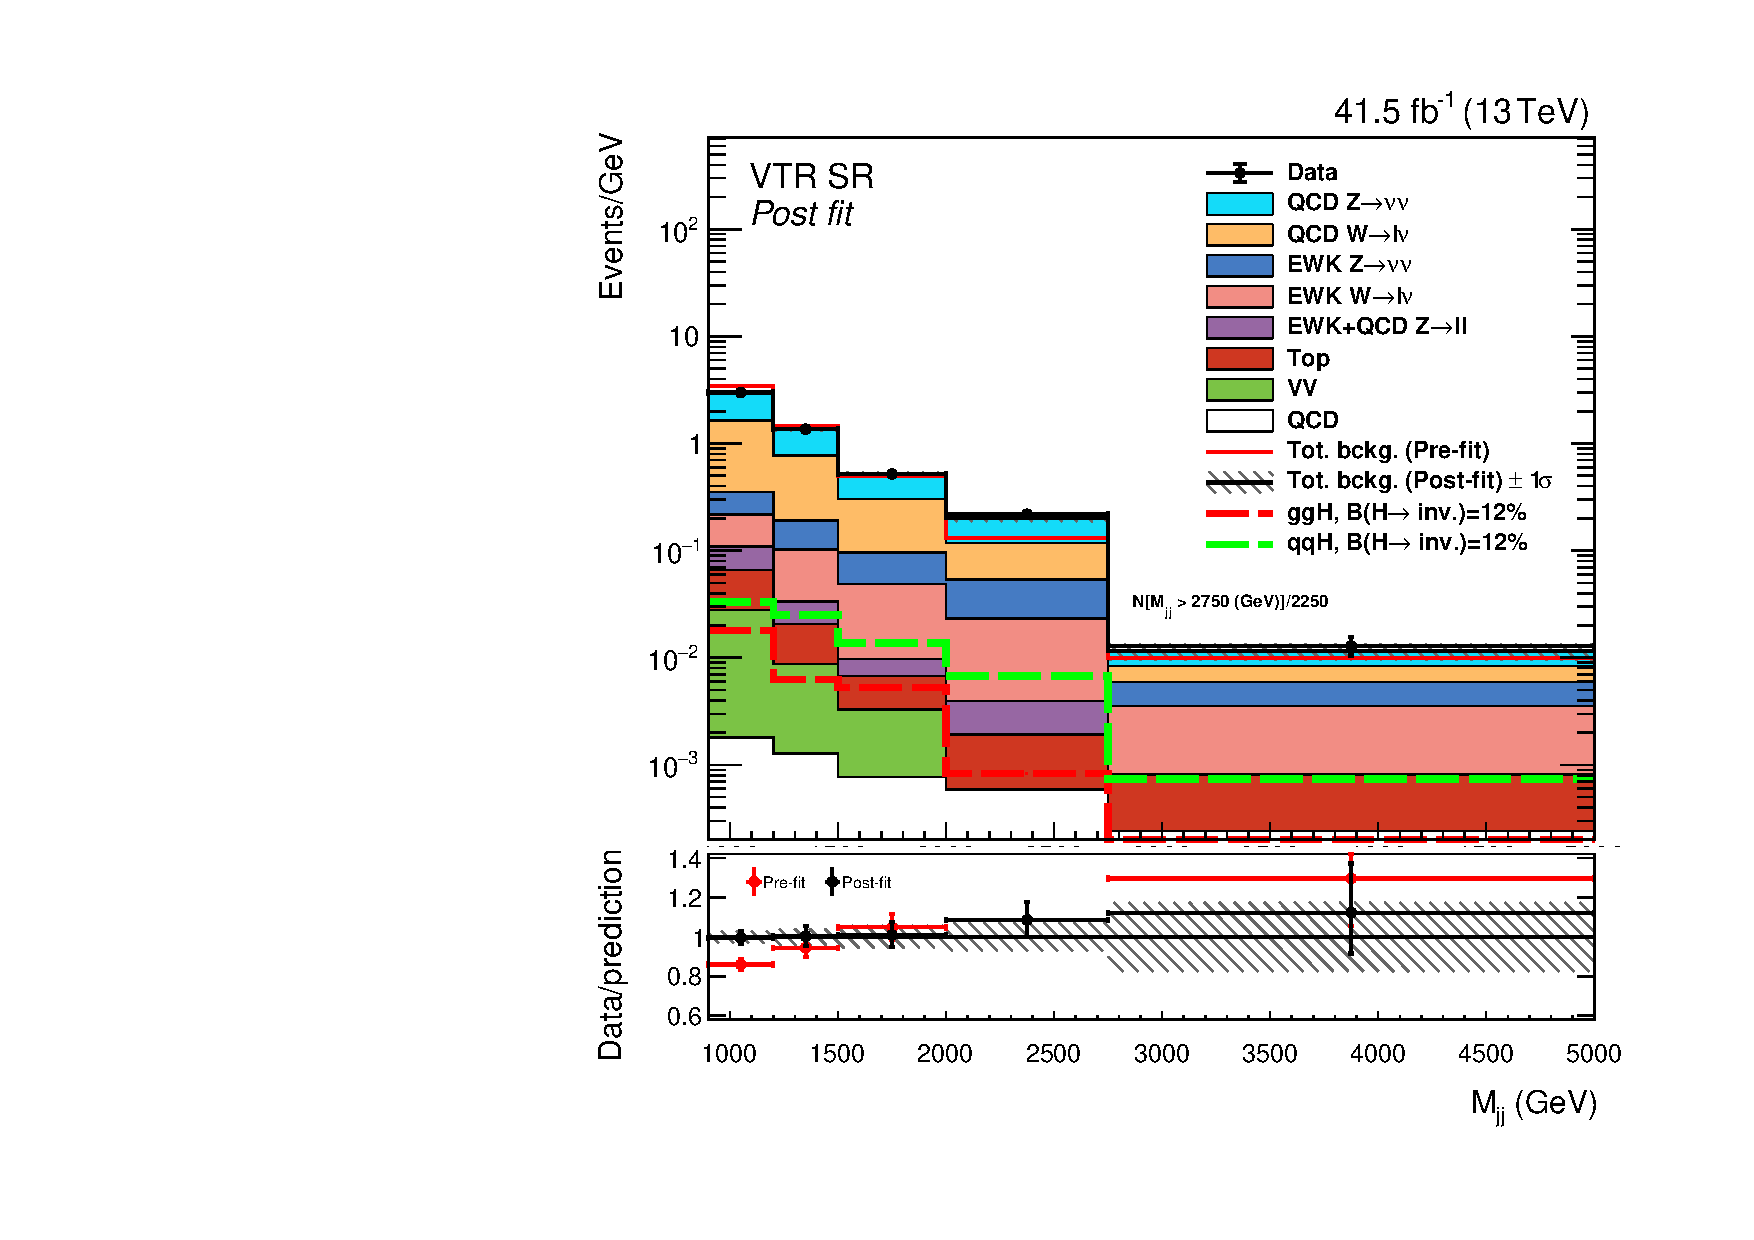
\includegraphics[width= 0.47\textwidth]{Results/SplusBFit/VTR_2017_SR.pdf}}
    \subfigure[VTR 2018]{
    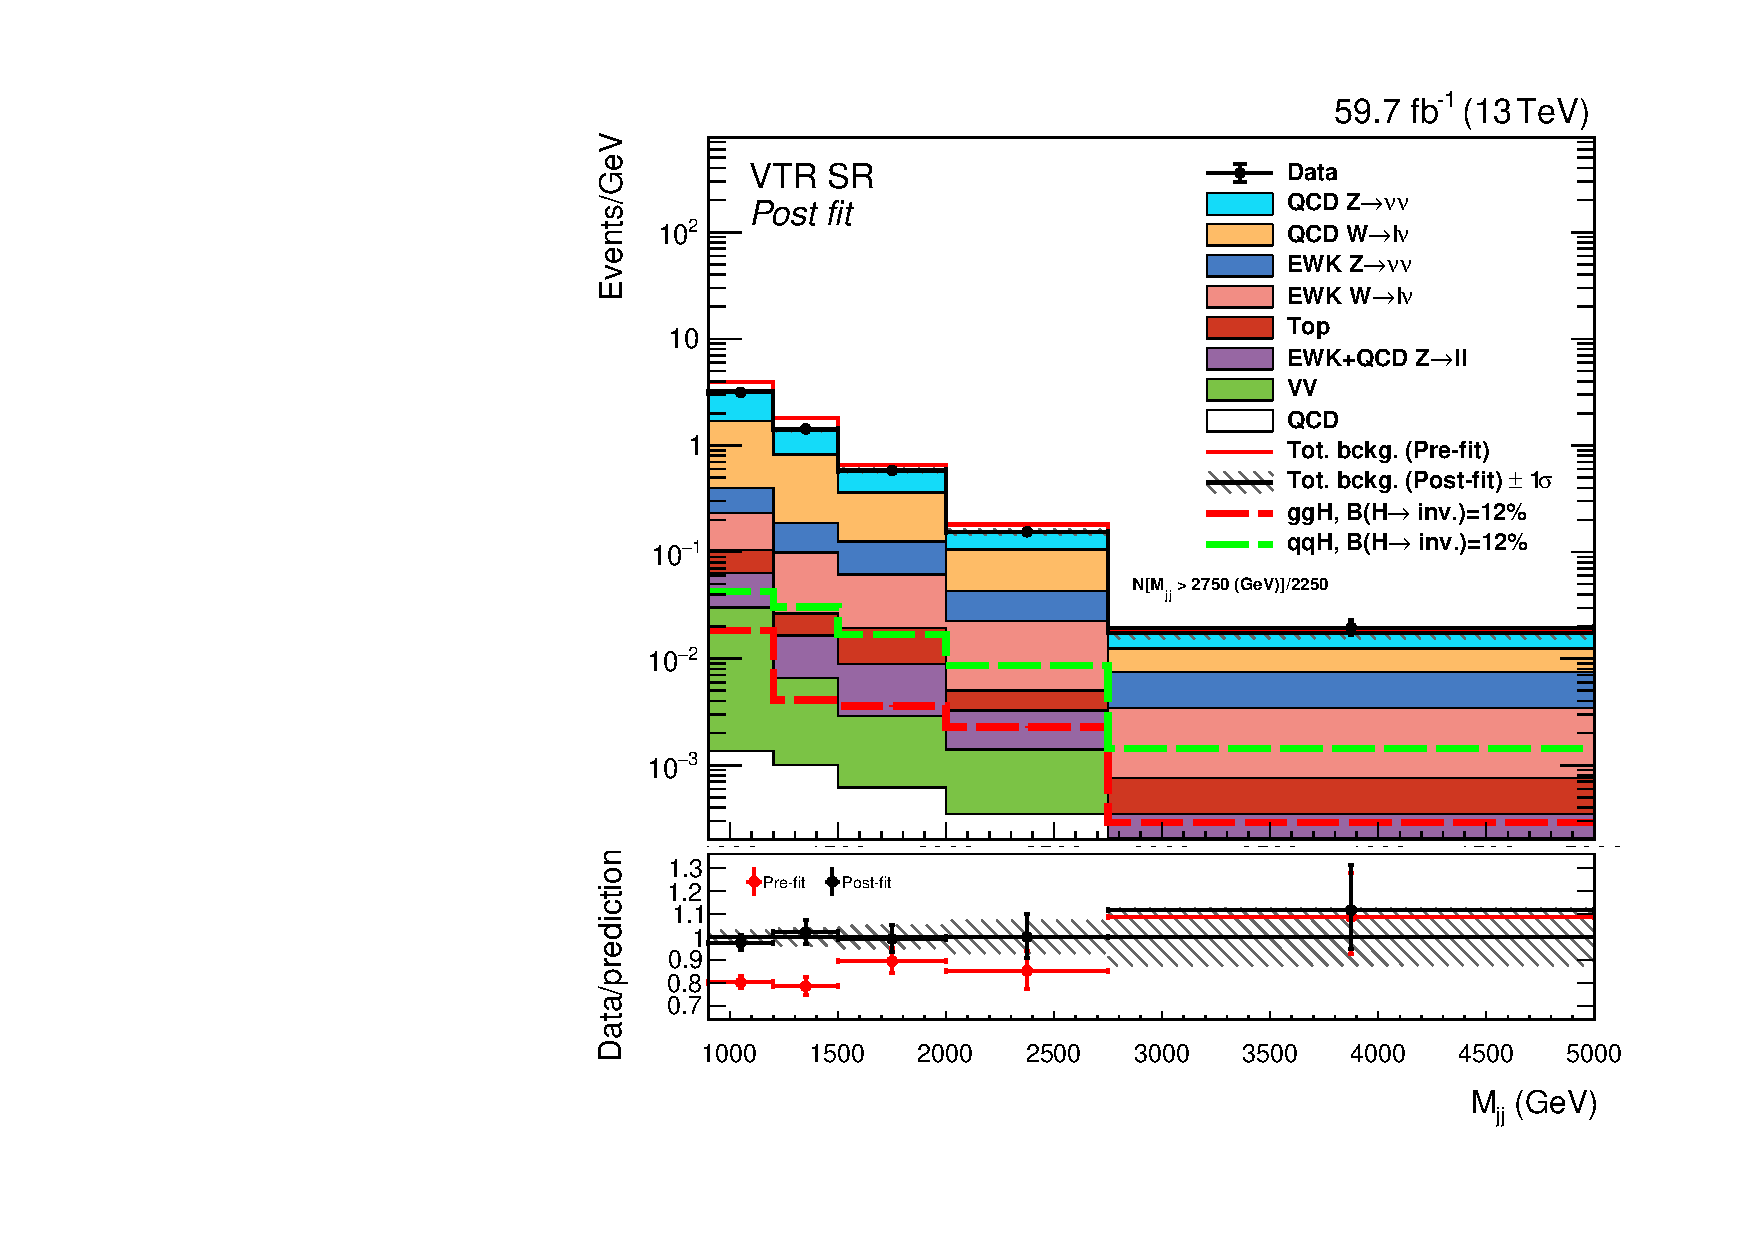
\includegraphics[width= 0.47\textwidth]{Results/SplusBFit/VTR_2018_SR.pdf}}
  \caption{Post-fit distributions for the SR, showing the: (a) MTR 2017, (b) MTR 2018, (c) VTR 2017 an (d) VTR 2018.}
  \label{fig:SR}
\end{figure}


\begin{figure}[htbp]
  \centering
   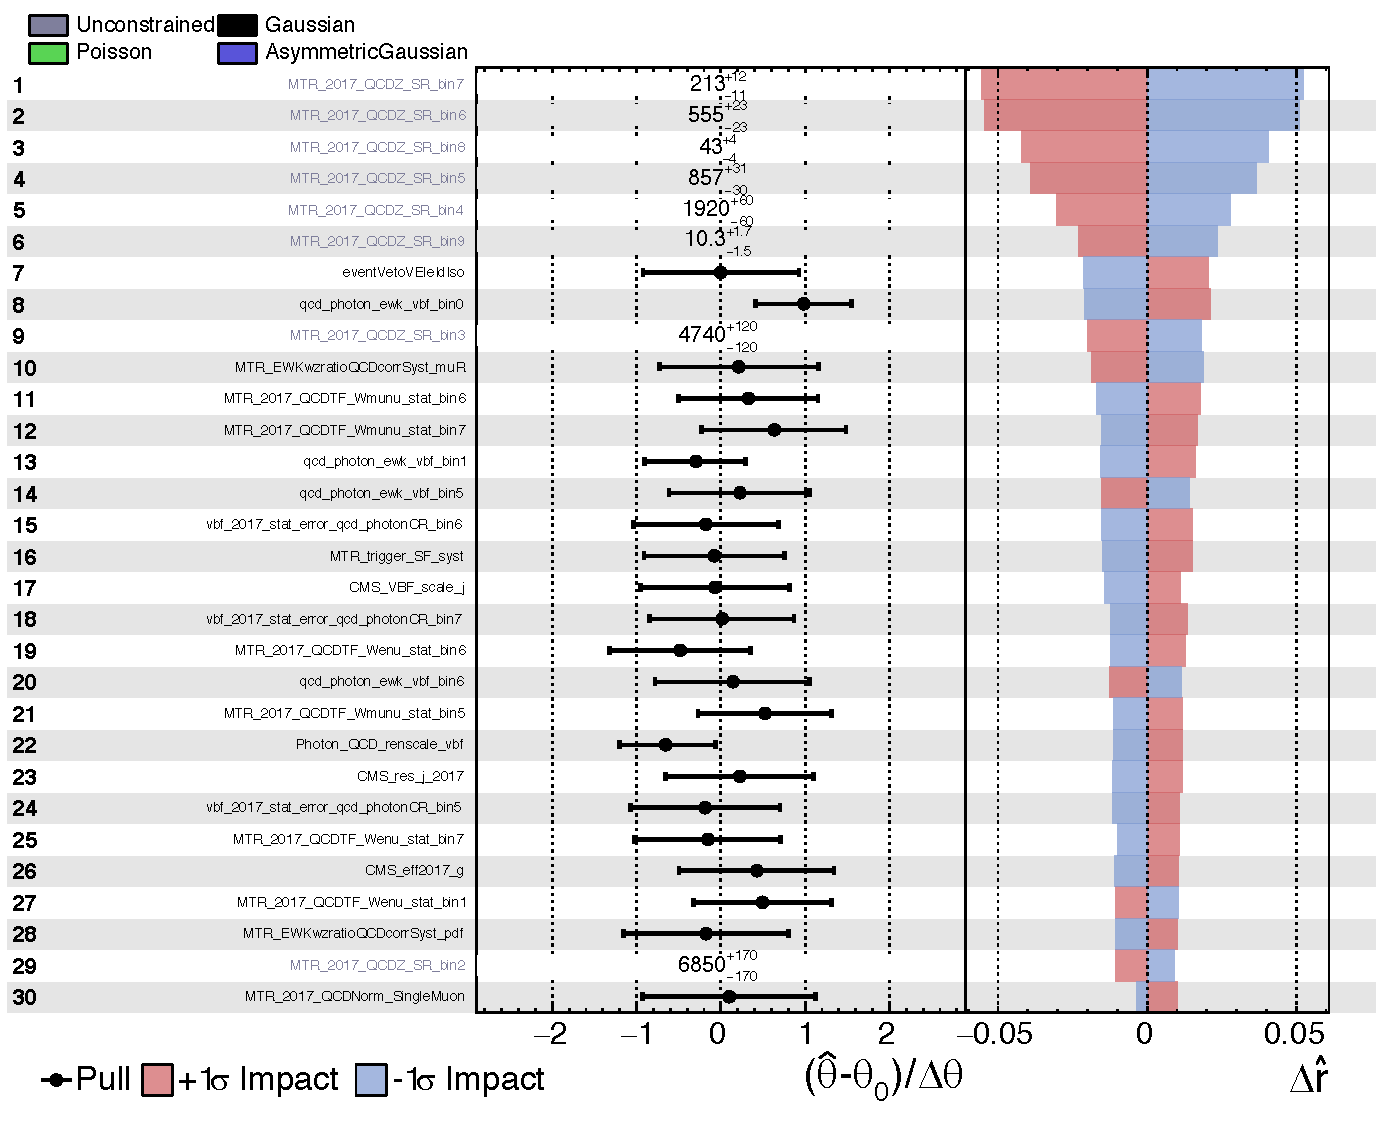
\includegraphics[width=\textwidth]{FIt_structure/impacts_perchannel_MTR_2017_p1.pdf}
   
  \caption{Impacts of the nuisance parameters from the final fit for the MTR category for 2017 data. The left panel shows the difference between the post and pre-fit value of the nuisance parameter divided by its pre-fit uncertainty. The parameter $\Delta r$ in the right panel shows the difference between the the best fit value of Br(H$\rightarrow$inv) after setting the given nuisance parameter at $\pm\text{1}\sigma$ of its nominal value.}
  \label{app:impacts_MTR_2017}
\end{figure}



\begin{figure}[htbp]
  \centering
   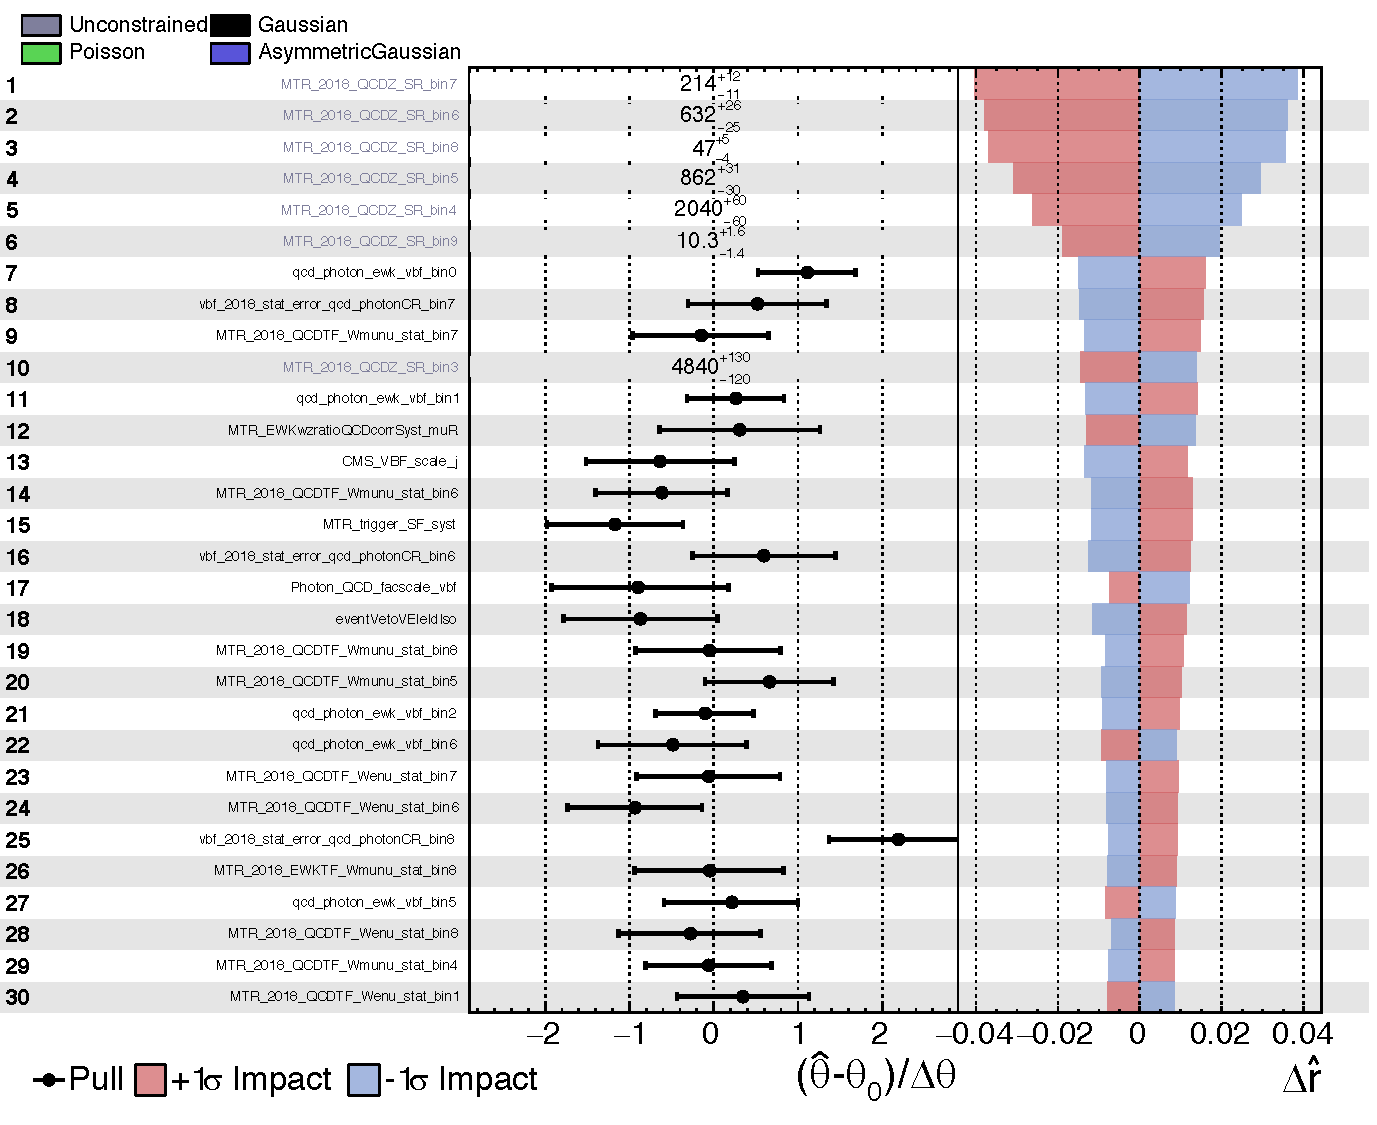
\includegraphics[width=\textwidth]{FIt_structure/impacts_perchannel_MTR_2018_p1.pdf}
   
  \caption{Impacts of the nuisance parameters from the final fit for the MTR category for 2018 data. The panel details follow the convention introduced in~\ref{app:impacts_MTR_2017}.}
  \label{app:impacts_MTR_2018}
\end{figure}


\begin{figure}[htbp]
  \centering
   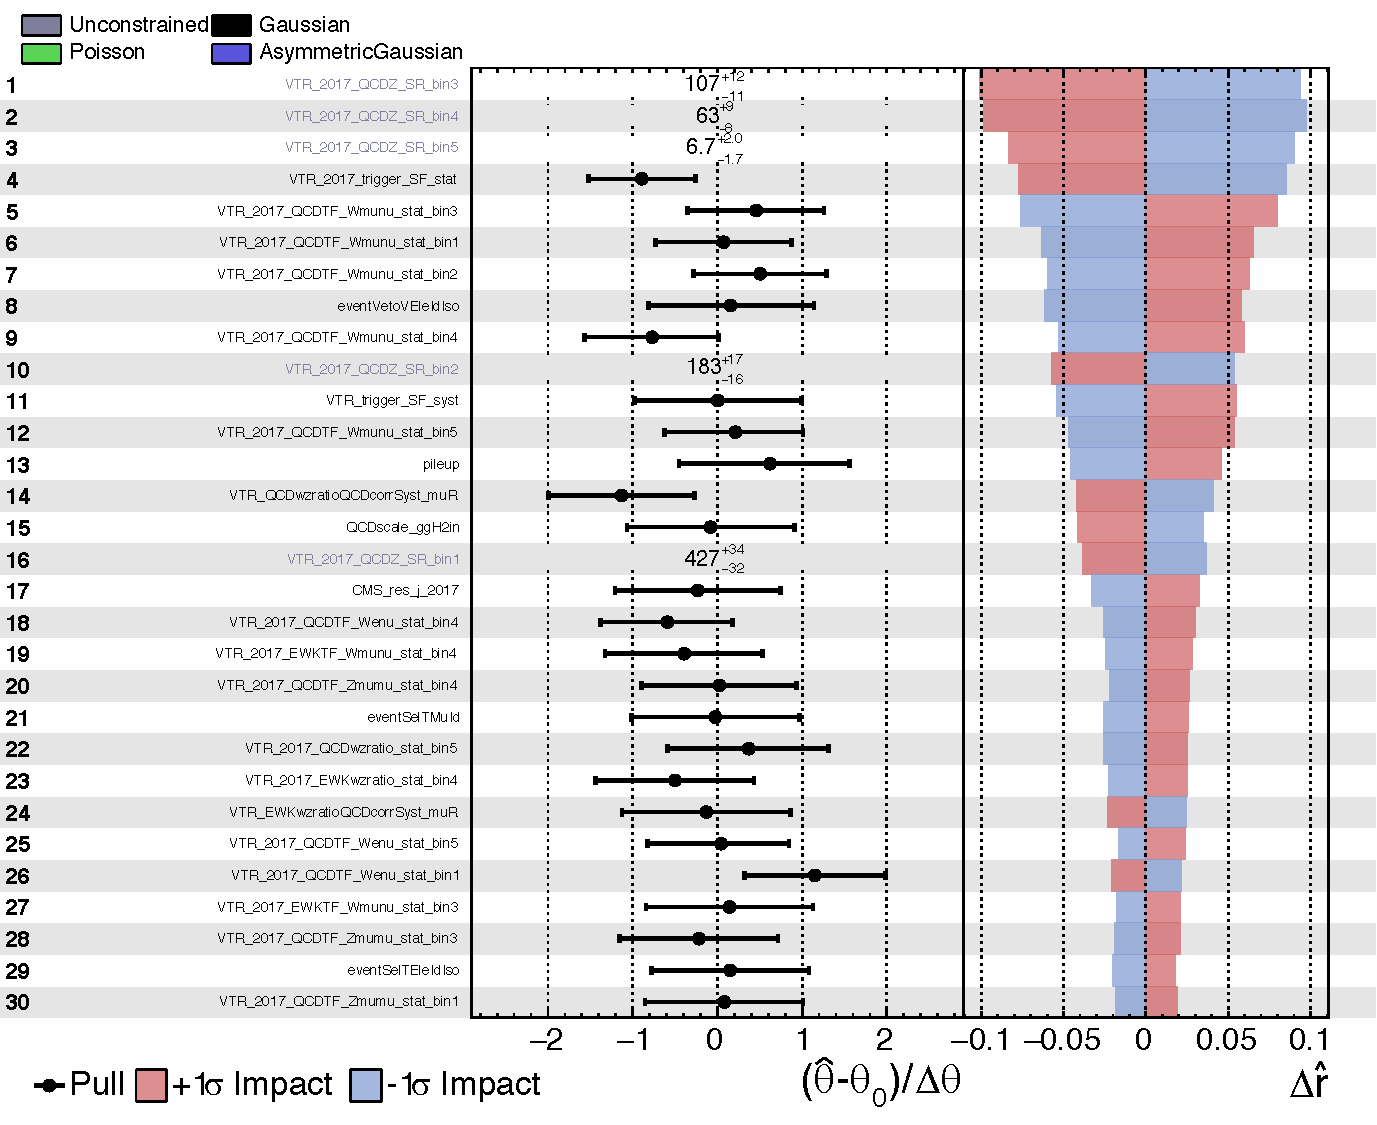
\includegraphics[width=\textwidth]{FIt_structure/impacts_perchannel_VTR_2017_p1.pdf}
   
  \caption{Impacts of the nuisance parameters from the final fit for the VTR category for 2017 data. The panel details follow the convention introduced in~\ref{app:impacts_MTR_2017}.}
  \label{app:impacts_VTR_2017}
\end{figure}

\begin{figure}[htbp]
  \centering
   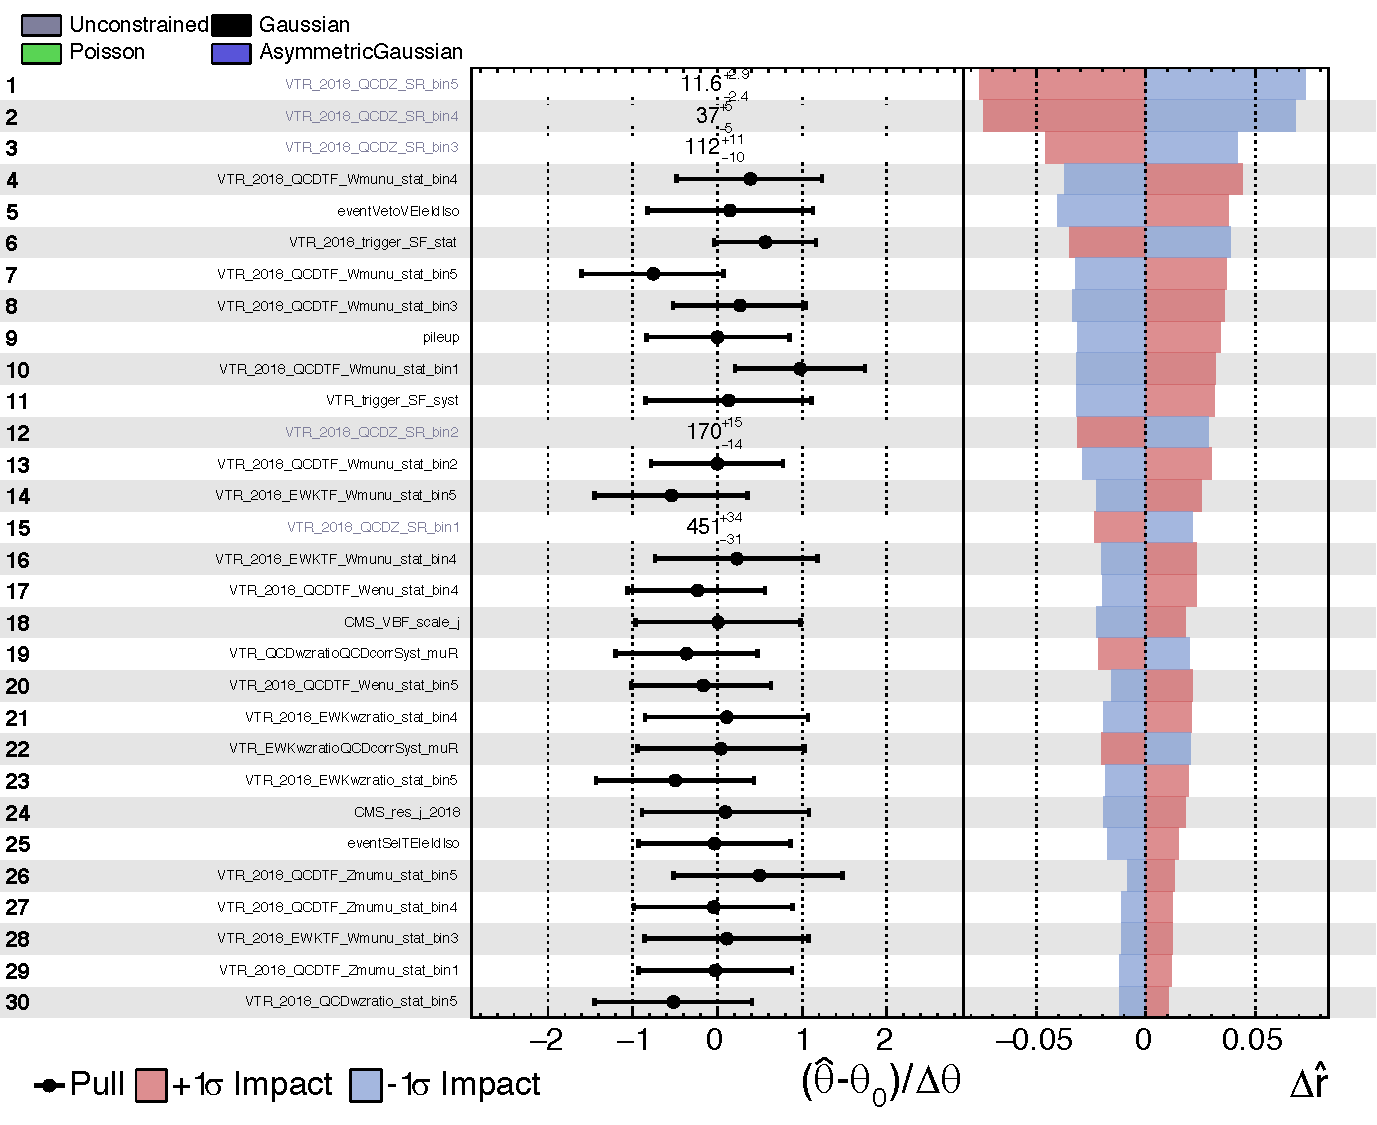
\includegraphics[width=\textwidth]{FIt_structure/impacts_perchannel_VTR_2018_p1.pdf}
   
  \caption{Impacts of the nuisance parameters from the final fit for the VTR category for 2018 data. The panel details follow the convention introduced in~\ref{app:impacts_MTR_2017}.}
  \label{app:impacts_VTR_2018}
\end{figure}





\hspace{10pt} The fit procedure, following the CLs technique, yiled a 95~\% CL upper limit on the Br(H$\rightarrow$ inv), under the assumption of a SM Higgs boson with $m_{H} = $125.09~GeV. For the analysis focusing on the 2017 and 2018 data taking periods (with a total luminosity of 101.2~fb$^{-1}$), it places an observed (expected) 95~\% CL upper limit on Br(H$\rightarrow$inv) to be 0.15 (0.13). The combination with the study focusing on the 2016 data states a limit of Br(H$\rightarrow$inv)~$<$~0.15 (0.12). The per category limits and subsequent combinations (for 2017 and 2018 data) are summarised in Table~\ref{tab:limits}.

\hspace{10pt} A discrepancy between the observed and the expected limit can be seen in 2017 data results where it appears in both the independent, MTR and VTR, categories (for VTR the difference is slightly larger than 1$\sigma$). The reason behind this could be an additional source of background that was not properly accounted for (possibly seen in the excess in relevant SR $m_{jj}$ distributions for $m_{jj}>$~2000~GeV)\footnote{Similar discrepancy was observed in the study focusing on the 2016 data~\cite{paper:HIG_17_023}.}. The supporting fact that this is not an appearance of signal is that the "observed to estimated" limit agreement for the 2018 era is much better across both categories\footnote{Detailed study of the 2017 era is currently ongoing within the CMS collaboration.}.

\begin{table*}[h!]
    \centering
    \begin{tabular}{l c c c c}
       \hline
       Category & Observed  & Expected  & 1-$\sigma$ interval & 2-$\sigma$ interval \\
       \hline
                      MTR 2017  & 0.26  & 0.22  & [0.16 -- 0.31]  & [0.12 -- 0.43] \\ 
                      VTR 2017  & 0.81  & 0.53  & [0.38 -- 0.76] & [0.29 -- 1.04]\\
                      MTR 2018  & 0.17  & 0.17  & [0.12 -- 0.24]  & [0.09 -- 0.32] \\ 
                      VTR 2018  & 0.33  & 0.33  & [0.23 -- 0.47]  & [0.18 -- 0.64]\\
                 MTR 2017 2018  & 0.15  & 0.14  & [0.10 -- 0.20]  & [0.08 -- 0.27] \\ 
                      all 2017  & 0.28  & 0.21  & [0.15 -- 0.30]  & [0.12 -- 0.41] \\ 
                      all 2018  & 0.15  & 0.15  & [0.11 -- 0.22]  & [0.08 -- 0.30] \\ 
                 all 2017 2018  & 0.15  & 0.13  & [0.10 -- 0.19]  & [0.07 -- 0.25] \\ 
                          Run2  & 0.15  & 0.12  & [0.08 -- 0.16]  & [0.06 -- 0.22] \\ 
       \hline
    \end{tabular}
    \caption{Summary of results expressed as 95~\%~CL upper limit on the Br(H$\rightarrow$inv). Contributions from each category and their subsequent combinations are presented, culminating with the result combining all Run 2 studies. }
    \label{tab:limits}
\end{table*}

\hspace{10pt} The size of the contribution from different sources of uncertainties can be obtained by freezing groups of nuisance parameters (being grouped by their common origin): theory (as introduced in Section~\ref{sec:theory_uncert}), statistical precision of simulation samples, lepton/photon efficiencies, jet calibration (jet energy scale and resolution), trigger and other (covering the multijet estimate, effects on smaller backgrounds, pile-up, etc). This leads to the following result expressed for the best fit\footnote{The SM prediction for the Br(H$\rightarrow$inv) stands at $\sim$~0.1~\%.}:
\begin{equation} 
\begin{split}
\text{Br(H}\rightarrow \text{inv)} & = 0.045 ^{+0.060}_{-0.061}\\
        & = 0.045 ^{+0.029}_{-0.030} (\mathrm{theory}) ^{+0.028}_{-0.028} (\mathrm{sim. stat.}) ^{+0.014}_{-0.15} (\mathrm{lepton/photon~eff}) \\
        & ~ \pm 0.004 (\mathrm{jet~calib.}) 
         ^{+0.021}_{-0.022} (\mathrm{trigger}) ^{+0.017}_{-0.015} (\mathrm{other})\pm 0.032 (\mathrm{stat.}),
\end{split}
\end{equation}

where it can be seen that this analysis is systematically limited with the main contribution originating from theoretical uncertainties and the statistical precision of simulation samples. This is graphically summarised in Figure~\ref{app:obs_best_fit} (while a corresponding breakdown for the best "blinded" fit can be found in Figure~\ref{app:est_best_fit}).
\begin{figure}[htbp]
  \centering
   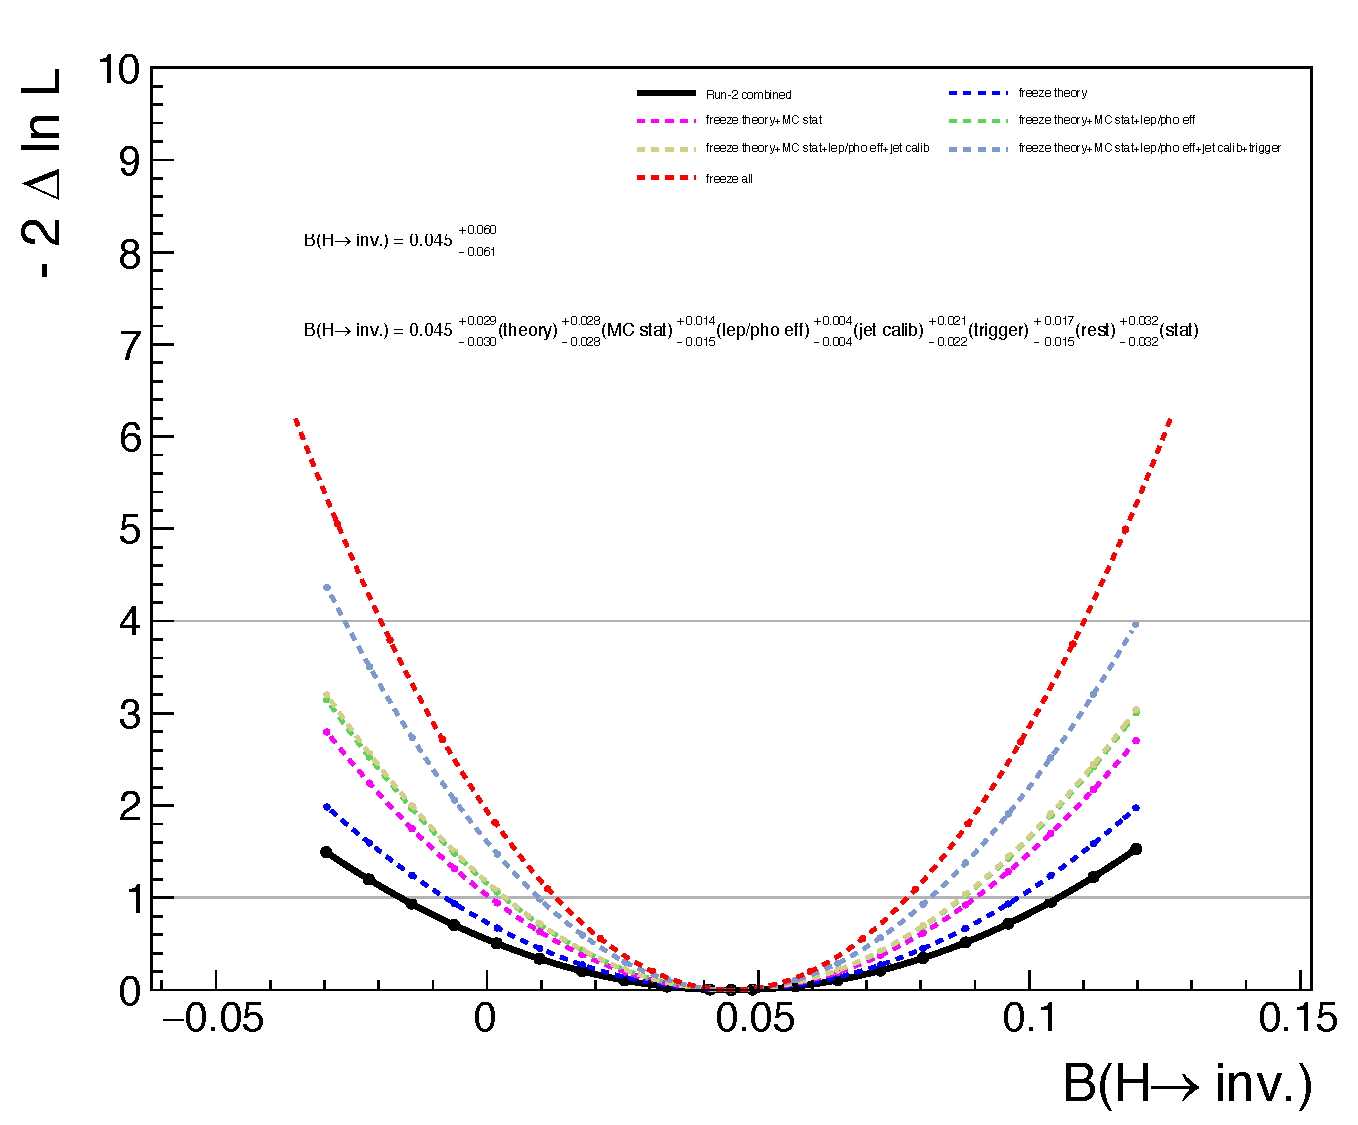
\includegraphics[width=\textwidth]{FIt_structure/breakdown.pdf}
   
  \caption{Likelihood scan for the Run 2 combination for the best fit Br(H$\rightarrow$inv) = 0.045, with scans obtained by sequentially freezing the groups of nuisance parameters.}
  \label{app:obs_best_fit}
\end{figure}

\newpage
\hspace{10pt} Finally, a comparison with direct DM detection experiments using the procedure introduced in Chapter~\ref{ch:Higgs_LHC_DM} is made. The observed limit for the combined measurement describing the Run 2 phase is presented as a 90\% CL upper limit in order to be comparable with the results from direct DM searches following the previously introduced strategy. This result is shown in Figure~\ref{fig:dm_run2} comparing the measurement form the CMS experiment with those coming from LUX~\cite{DM:lux}, CDMS~\cite{DM:cdsmlite}, XENON~\cite{DM:xenon1,DM:xenon2}, CRESST~\cite{DM:cresst} and PandaX-II~\cite{DM:panda} collaborations. Following the introduction of Equations~\ref{eq:xs_scalar}-\ref{eq:xs_ferm} for the scalar and fermion scenario, it can be seen that the limitation of the used method, seen in both lines for $m_{DM}~\approx~\frac{m_{H}}{2}$, is arising due to the factor $\beta = \sqrt{1-\frac{4m_{DM}^2}{m_{H}^2}}$. On the other end of $m_{DM}$, the mass range stops at 1~GeV due to the assumed Higgs portal model not being sustainable for DM particles located within the mass order of quark masses. Lastly, the difference between the two curves (red and orange) is arising from the different dependencies on the $m_{DM}$ assumed by the model, being best seen in Equations~\ref{eq:xs_scalar} and \ref{eq:xs_ferm}.


  \begin{figure}[htbp]
    \begin{center}
        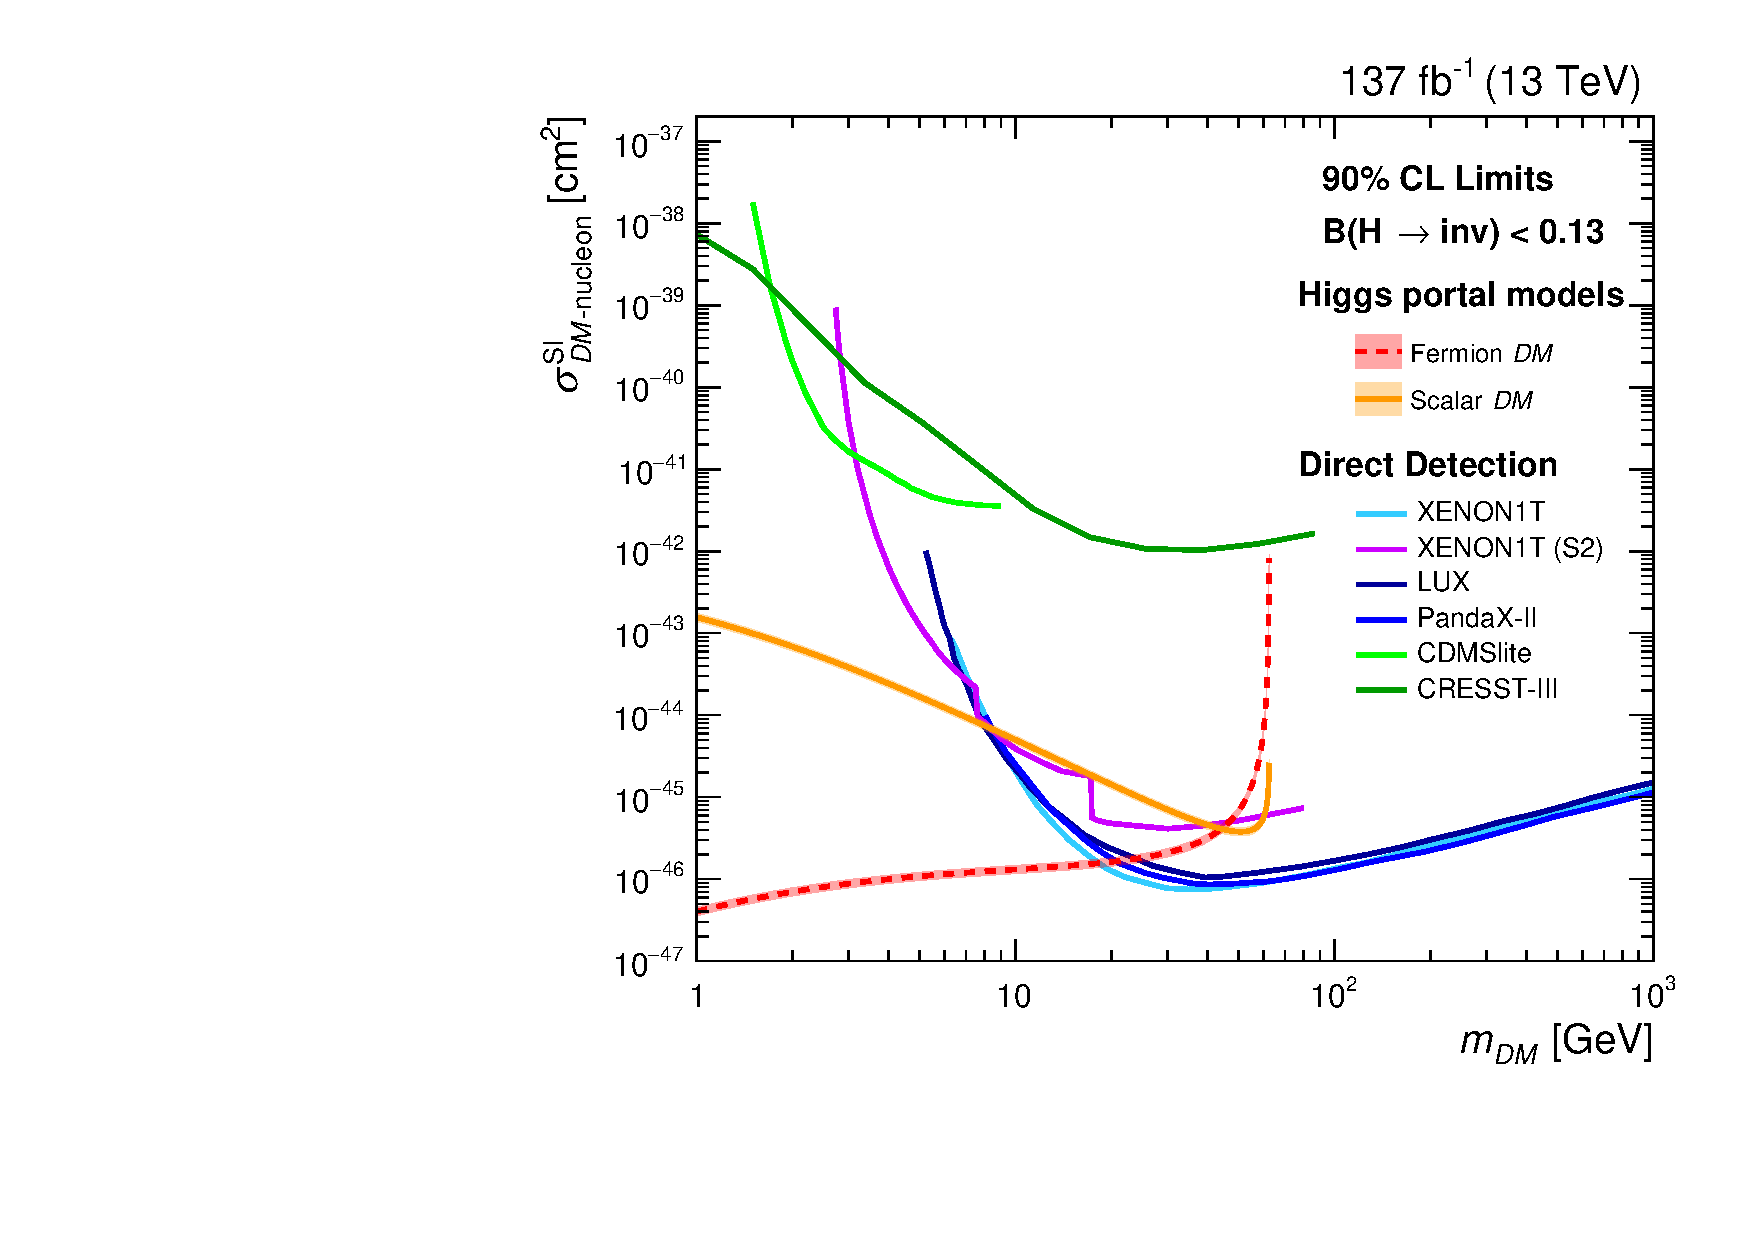
\includegraphics[width=0.9\textwidth]{FIt_structure/higgsPortalDM.pdf}
        \caption{The reinterpretation of the CMS results in terms of the 90\% CL upper limits on the spin-independent DM-nulcleon scattering cross section when assuming a fermion (red) or a scalar (orange) DM particle (presented as a function of $m_{DM}$). Limits are compared with results originating from direct DM detection experiments.}
      \label{fig:dm_run2}
    \end{center}
  \end{figure}

\section{Summary}
\hspace{10pt} The presented study covered the search for the invisible decays of the Higgs boson, where the production mode in question is VBF. The study was performed using the 101.2~fb$^{-1}$ of data collected by the CMS experiment corresponding to the 2017 and 2018 years of operation. Exploration of additional phase space found in lower $E_{T,miss}$ range was enabled through the introduction of a new analysis category based on new trigger algorithms tailored to look for the VBF characteristics in events. No deviations from the SM have been observed. The result is interpreted as the observed (expected) 95\% CL upper limit on the branching ratio of the Higgs boson decaying invisibly and it stands at: Br(H$\rightarrow$inv) = 0.15 (0.13). A combination with previous measurements targeting the VBF topology during the Run 2 phase is presented, bringing the total integrated luminosity to 137.1~fb$^{-1}$. The observed (expected) value of the Br(H$\rightarrow$inv) for the entire Run 2 phase is found to be 0.15 (0.12). Figure~\ref{fig:combined_limit} summarises the results of the individual measurements and the subsequent combination of categories.

\begin{figure}[htbp]
  \centering
    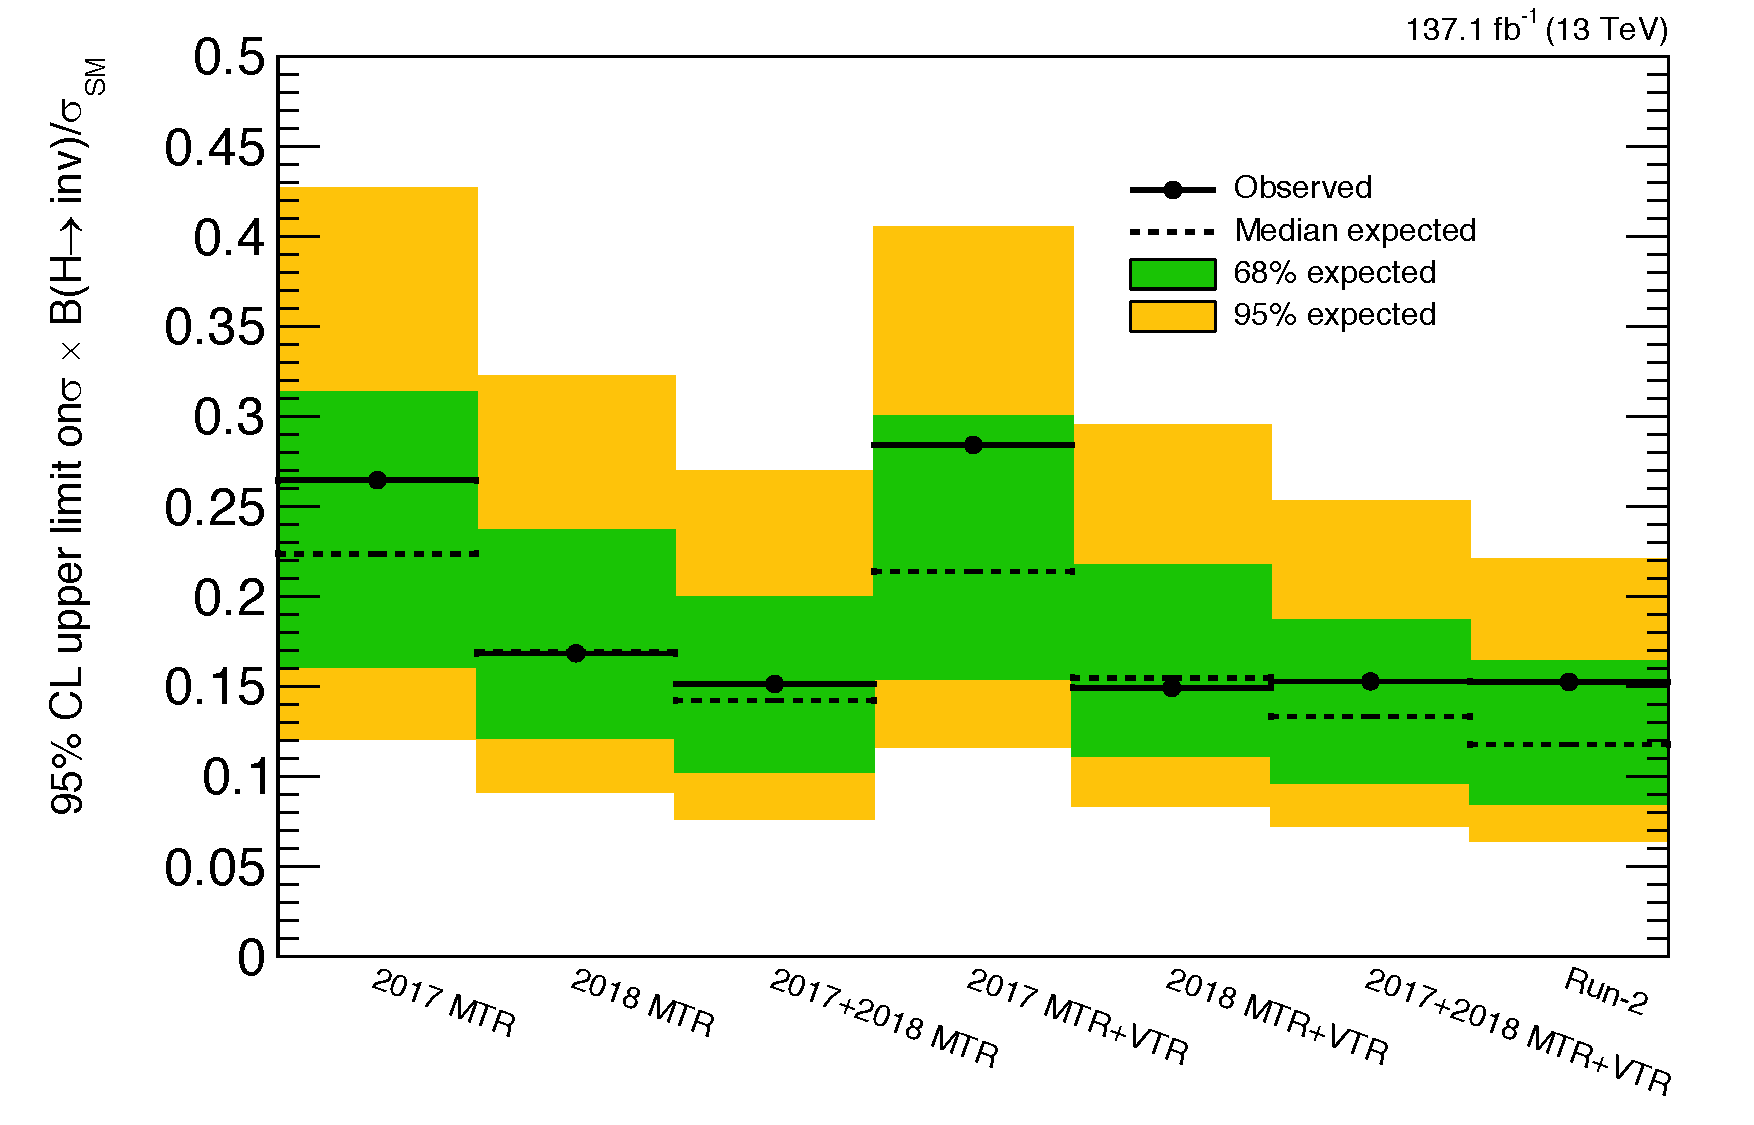
\includegraphics[width= 0.95\textwidth]{Results/limit_unblinded.pdf}
  \caption{Final limits for the Run 2 phase showing the contribution from each of the categories.}
  \label{fig:combined_limit}
\end{figure}